%%Para utilizar este template siga o tutorial disponível em http://www.biblioteca.ufc.br/wp-content/uploads/2015/09/tutorial-sharelatex.pdf
%%%%%%%%%%%%%%%%%%%%%%%%%%%%%%%%%%%%%%%%%%%%%%%%%%%%%%%
%% Você deve criar uma conta no Overleaf. Depois,    %%
%% vá nas opções no canto esquerdo superior da tela  %%
%% e clique em "Copiar Projeto". Dê um novo nome pa- %%
%% ra o projeto.                                     %%
%%                                                   %%
%% Os principais desenvolvedores deste template são: %%
%%                                                   %%
%%            Ednardo Moreira Rodrigues              %%
%%       (Doutor em Engenharia Elétrica - UFC)       %%
%%(Coord. do Grupo de Astronomia da Seara da Ciência)%%
%%                      &                            %%
%%            Alan Batista de Oliveira               %%
%%           (Engenheiro Eletricista - UFC)          %%
%%                                                   %%
%% Consultoria Bibliotecária                         %%
%%                                                   %%
%%  Versão 2016 - ShareLaTeX:                        %% 
%%                                                   %%
%% - Francisco Edvander Pires Santos;                %%
%% - Juliana Soares Lima;                            %%
%% - Izabel Lima dos Santos;                         %%
%% - Kalline Yasmin Soares Feitosa;                  %%
%% - Eliene Maria Vieira de Moura.                   %%
%% ------------------------------------------------- %% 
%%  Versão 2019,2020 - Overleaf:                     %%
%%                                                   %%
%%  Biblioteca de Ciências Humanas:                  %%
%% - Francisco Edvander Pires Santos;                %%
%% - Juliana Soares Lima;                            %%
%% - Eliene Maria Vieira de Moura;                   %%
%% - Edmundo Moreira de Sousa Filho.                 %%
%%                                                   %%
%% Biblioteca da FEAAC:                              %%
%% - Izabel Lima dos Santos;                         %%
%% - Kalline Yasmin Soares Feitosa;                  %%
%% - Kleber Lima dos Santos.                         %%
%%                                                   %%
%%  Biblioteca do Curso de Física:                   %%
%% - Aline Rodrigues de Lima Mendes;                 %%
%% - Maria de Jesus Silva dos Santos.                %%
%%                                                   %%
%%  Biblioteca Central do Campus do Pici:            %%
%% - Raquel da Silva Nascimento.                     %%
%% - Felipe Ferreira da Silva                        %%
%%  Versão 2019,2020 - Overleaf:                     %%
%%  ------------------------------------------------ %%
%%  Versão de 2022 - Overleaf                        %%
%%                                                   %%
%%   a) Felipe Ferreira da Silva                        %%
%%   b) Ednardo Moreira Rodrigues                       %%
%%   c) Comissão de Normalização do Sistema de          %%
%%      Bibliotecas da UFC                              %%
%%                                                   %%
%% Colaboradores                                     %%
%%                                                   %%
%% -Andrei Bosco Bezerra Torres                      %% 
%% (Professor - Sistemas e Mídias Digitais -         %%
%% Instituto Universidade Virtual - UFC)             %%
%% Tiago Alves Lima                                  %% 
%% (Aluno de Mestrado em Eng. Elétrica)              %%
%%                                                   %%
%% Grande parte do trabalho foi adaptado do template %%
%% da UECE elaborado por:                            %%
%% Thiago Nascimento  (UECE)                         %%
%% Project available on:                             %%
%% https://github.com/thiagodnf/uecetex2             %%
%%                                                   %%
%% "Dúvidas, esclarecimentos ou sugestões podem ser  %%
%% enviadas para o seguinte e-mail:                  %%
%%                                                   %%
%%             bu@ufc.br               %%
%%                                                   %%
%% As últimas atualizações estão descritas no inicio %%
%% do arquivo "README.md".                           %%
%%                                                   %%
%%%%%%%%%%%%%%%%%%%%%%%%%%%%%%%%%%%%%%%%%%%%%%%%%%%%%%%

% % With warning !!
% \documentclass[        
%     a4paper,          % Tamanho da folha A4
%     12pt,             % Tamanho da fonte 12pt
%     chapter=TITLE,    % Todos os capitulos devem ter caixa alta
%     section=Title,    % Todas as secoes devem ter caixa alta somente na primeira letra
%     subsection=Title, % Todas as subsecoes devem ter caixa alta somente na primeira letra
%     oneside,          % Usada para impressao em apenas uma face do papel
%     english,          % Hifenizacoes em ingles
%     spanish,          % Hifenizacoes em espanhol
%     brazil,           % Ultimo idioma eh o idioma padrao do documento
%     fleqn             % Comente esta linha se quiser centralizar as equacoes. Comente também a linha 65 abaixo
% ]{abntex2}


\documentclass[        
    a4paper,          % Tamanho da folha A4
    12pt,             % Tamanho da fonte 12pt
    chapter=TITLE,    % Todos os capitulos devem ter caixa alta
%    section=Title,    % Todas as secoes devem ter caixa alta somente na primeira letra
%    subsection=Title, % Todas as subsecoes devem ter caixa alta somente na primeira letra
    oneside,          % Usada para impressao em apenas uma face do papel
    english,          % Hifenizacoes em ingles
    spanish,          % Hifenizacoes em espanhol
    brazil,           % Ultimo idioma eh o idioma padrao do documento
    fleqn             % Comente esta linha se quiser centralizar as equacoes. Comente também a linha 65 abaixo
]{abntex2}



% Para utilizar este template siga o tutorial disponível em http://www.biblioteca.ufc.br/wp-content/uploads/2015/09/tutorial-sharelatex.pdf

%%%%%%%%%%%%%%%%%%%%%%%%%%%%%%%%%%%%%%%%%%%%%%%%%%%%%%%
%% Você deve criar uma conta no Overleaf. Depois,    %%
%% vá nas opções no canto esquerdo superior da tela  %%
%% e clique em "Copiar Projeto". Dê um novo nome pa- %%
%% ra o projeto.                                     %%
%%                                                   %%
%% Os principais desenvolvedores deste template são: %%
%%                                                   %%
%%            Ednardo Moreira Rodrigues              %%
%%       (Doutor em Engenharia Elétrica - UFC)       %%
%%(Coord. do Grupo de Astronomia da Seara da Ciência)%%
%%                      &                            %%
%%            Alan Batista de Oliveira               %%
%%           (Engenheiro Eletricista - UFC)          %%
%%                                                   %%
%% Consultoria Bibliotecária                         %%
%%                                                   %%
%%  Versão 2016 - ShareLaTeX:                        %% 
%%                                                   %%
%% - Francisco Edvander Pires Santos;                %%
%% - Juliana Soares Lima;                            %%
%% - Izabel Lima dos Santos;                         %%
%% - Kalline Yasmin Soares Feitosa;                  %%
%% - Eliene Maria Vieira de Moura.                   %%
%%                                                   %% 
%%  Versão 2019 - Overleaf:                          %%
%%                                                   %%
%%  Biblioteca de Ciências Humanas:                  %%
%% - Francisco Edvander Pires Santos;                %%
%% - Juliana Soares Lima;                            %%
%% - Eliene Maria Vieira de Moura;                   %%
%% - Edmundo Moreira de Sousa Filho.                 %%
%%                                                   %%
%% Biblioteca da FEAAC:                              %%
%% - Izabel Lima dos Santos;                         %%
%% - Kalline Yasmin Soares Feitosa;                  %%
%% - Kleber Lima dos Santos.                         %%
%%                                                   %%
%%  Biblioteca do Curso de Física:                   %%
%% - Aline Rodrigues de Lima Mendes;                 %%
%% - Maria de Jesus Silva dos Santos.                %%
%%                                                   %%
%%  Biblioteca Central do Campus do Pici:            %%
%% - Raquel da Silva Nascimento.                     %%
%% - Felipe Ferreira da Silva                        %%
%%                                                   %%
%% Colaboradores                                     %%
%%                                                   %%
%% -Andrei Bosco Bezerra Torres                      %% 
%% (Professor - Sistemas e Mídias Digitais -         %%
%% Instituto Universidade Virtual - UFC)             %%
%% Tiago Alves Lima                                  %% 
%% (Aluno de Mestrado em Eng. Elétrica)              %%
%%                                                   %%
%% Grande parte do trabalho foi adaptado do template %%
%% da UECE elaborado por:                            %%
%% Thiago Nascimento  (UECE)                         %%
%% Project available on:                             %%
%% https://github.com/thiagodnf/uecetex2             %%
%%                                                   %%
%% "Dúvidas, esclarecimentos ou sugestões podem ser  %%
%% enviadas para o seguinte e-mail:                  %%
%%                                                   %%
%%             atendimentobch@ufc.br                 %%
%%                                                   %%
%% As últimas atualizações estão descritas no inicio %%
%% do arquivo "README.md".                           %%
%%                                                   %%
%%%%%%%%%%%%%%%%%%%%%%%%%%%%%%%%%%%%%%%%%%%%%%%%%%%%%%%

%% Warnings and Info Supress to compile begin 
\usepackage{silence}
\WarningFilter{nameref}{ The definition of \label has changed! Check your packages! Replacing it with the kernel definition on input line}
\WarningFilter{glossaries}{Overriding \printglossary}     
\WarningFilter{glossaries}{Overriding `theglossary' environment }     
\WarningFilter{glossaries}{No \printglossary or \printglossaries found. (Remove \makeglossaries if you don't want any glossaries.) This document will not have a glossary.}     

%% Warnings and Info Supress to compile end

% \usepackage{hyperref}
% Importações de pacotes
\usepackage[utf8]{inputenc}                         % Acentuação direta
\usepackage[T1]{fontenc}                            % Codificação da fonte em 8 bits
\usepackage{graphicx}                               % Inserir figuras
\usepackage{amsfonts, amssymb, amsmath}             % Fonte e símbolos matemáticos
\usepackage{booktabs}                               % Comandos para tabelas
\usepackage{verbatim}                               % Texto é interpretado como escrito no documento
\usepackage{multirow, array}                        % Múltiplas linhas e colunas em tabelas
\usepackage{indentfirst}                            % Endenta o primeiro parágrafo de cada seção.
\usepackage{listings}                               % Utilizar codigo fonte no documento
\usepackage{xcolor}
\usepackage{microtype}                              % Para melhorias de justificação?
\usepackage[portuguese,ruled,lined]{algorithm2e}    % Escrever algoritmos
\usepackage{algorithmic}                            % Criar Algoritmos  
%\usepackage{float}                                 % Utilizado para criação de floats
\usepackage{amsgen}
\usepackage{lipsum}                                 % Usar a simulação de texto Lorem Ipsum
%\usepackage{titlesec}                              % Permite alterar os títulos do documento
% \usepackage{tocloft}                                % Permite alterar a formatação do Sumário
\usepackage{tocloft}

\usepackage{etoolbox}                               % Usado para alterar a fonte da Section no Sumário
\usepackage[nogroupskip,nonumberlist]{glossaries}   % Permite fazer o glossario. A apcao "sort=use" faz com que as siglas aparecam na lista conformse sao usadas no texto.

\usepackage[format=plain,justification=justified,skip=0pt,singlelinecheck = false,labelsep=colon]{caption}            % Altera o comportamento da tag caption. Algumas opcoes do caption so podem ser alternada no arquivo "antex2.cls, linhas 334 a 348.

\usepackage[alf, abnt-emphasize=bf, recuo=0cm, abnt-etal-cite=2, abnt-etal-list=0, abnt-etal-text=it]{lib/abntex2cite}  % Citações padrão UFC/ABNT NBR 6023 de 2018
%\usepackage[bottom]{footmisc}                      % Mantém as notas de rodapé sempre na mesma posição
%\usepackage{times}                                 % Usa a fonte Times
%%%%%%%%%%%%%%%%%%% AVISO %%%%%%%%%%%%%%%%%%%%%%%%%%%%%%%%%%%%%%%%
%descomente as duas linhas abaixo para alterar o texto de Times New Roman para Arial:

%\usepackage{helvet}
%\renewcommand{\familydefault}{\sfdefault}  % Usa a fonte Arial              
%%%%%%%%%%%%%%%%%%%%%%%%%%%%%%%%%%%%%%%%%%%%%%%%%%%%%%%%%%%%%%%%%%

\usepackage{mathptmx}         % Usa a fonte Times New Roman			%\usepackage{lmodern}         % Usa a fonte Latin Modern
%\usepackage{subfig}          % Posicionamento de figuras
%\usepackage{scalefnt}        % Permite redimensionar tamanho da fonte
%\usepackage{color, colortbl} % Comandos de cores
%\usepackage{lscape}          % Permite páginas em modo "paisagem"
%\usepackage{ae, aecompl}     % Fontes de alta qualidade
%\usepackage{picinpar}        % Dispor imagens em parágrafos
%\usepackage{latexsym}        % Símbolos matemáticos
%\usepackage{upgreek}         % Fonte letras gregas
\usepackage{appendix}         % Gerar o apendice no final do documento
\usepackage{paracol}          % Criar paragrafos sem identacao
\usepackage{lib/abntex2cite}
\usepackage{lib/ufcTex}	      % Biblioteca com as normas da UFC para trabalhos academicos
\usepackage{pdfpages}         % Incluir pdf no documento
\usepackage{amsmath}          % Usar equacoes matematicas
%\usepackage[opções]{subfigure} %plotar subfiguras


\makeglossaries % Organiza e gera a lista de abreviaturas, simbolos e glossario
\makeindex      % Gera o Indice do documento         

\renewcommand{\labelitemi}{\textendash} %Altera os marcadores de itemize para 

% \color{teal}



\setlength{\mathindent}{0pt} %Complementa o alinhamento de equações para totalmente a esquerda.

%%%%%%%%%%%%%%%%%%%%%%%%%%%%%%%%%%%%%%%%%%%%%%%%%%%%%
%%                     ATENCAO                     %%
%%%%%%%%%%%%%%%%%%%%%%%%%%%%%%%%%%%%%%%%%%%%%%%%%%%%%
%  Qual e o nivel do trabalho academico que voce esta 
% escrevendo? Retire o simbolo "%" apenas de um dos 
% quatro topicos abaixo refente ao nível do seu traba
% -lho.

%\trabalhoacademico{tccgraduacao}
%\trabalhoacademico{tccespecializacao}
\trabalhoacademico{dissertacao}
%\trabalhoacademico{tese}

%%%%%%%%%%%%%%%%%%%%%%%%%%%%%%%%%%%%%%%%%%%%%%%%%%%%%

% Define se o trabalho e uma qualificacao
% Coloque 'nao' para versao final do trabalho

\ehqualificacao{nao}

% Remove as bordas vermelhas e verdes do PDF gerado
% Coloque 'sim' pare remover

\removerbordasdohyperlink{sim} 

% Adiciona a cor Azul a todos os hyperlinks

\cordohyperlink{nao}

%%%%%%%%%%%%%%%%%%%%%%%%%%%%%%%%%%%%%%%%%%%%%%%%%%%%%
%%         Informacao sobre a instituicao          %%
%%%%%%%%%%%%%%%%%%%%%%%%%%%%%%%%%%%%%%%%%%%%%%%%%%%%%

\ies{Universidade Federal do Ceará}
\iessigla{UFC}
\centro{Centro de Tecnologia}
\departamento{Departamento de Engenharia Elétrica}

%%%%%%%%%%%%%%%%%%%%%%%%%%%%%%%%%%%%%%%%%%%%%%%%%%%%%
%%        Informacao para TCC de Graduacao         %%
%%%%%%%%%%%%%%%%%%%%%%%%%%%%%%%%%%%%%%%%%%%%%%%%%%%%%

\graduacaoem{Engenharia Xxxxxxx}
\habilitacao{bacharel} % Ou licenciado(a)

% AVISO: Caso necessario alterar o texto de apresenta-
% cao da Especializacao, ir a pasta "lib", arquivo 
% "ufctex.sty" na linha 502.


%%%%%%%%%%%%%%%%%%%%%%%%%%%%%%%%%%%%%%%%%%%%%%%%%%%%%
%%     Informacao para TCC de Especializacao       %%
%%%%%%%%%%%%%%%%%%%%%%%%%%%%%%%%%%%%%%%%%%%%%%%%%%%%%

\especializacaoem{Yyyyyyyyy}

% AVISO: Caso necessario alterar o texto de apresenta-
% cao da Especializacao, ir a pasta "lib", arquivo 
% "ufctex.sty" na linha 507.

%%%%%%%%%%%%%%%%%%%%%%%%%%%%%%%%%%%%%%%%%%%%%%%%%%%%%
%%         Informacao para Dissertacao             %%
%%%%%%%%%%%%%%%%%%%%%%%%%%%%%%%%%%%%%%%%%%%%%%%%%%%%%

\programamestrado{Programa de Pós-Graduação em Engenharia Elétrica}
\nomedomestrado{Mestrado Acadêmico em Engenharia Elétrica}
\mestreem{Engenharia Elétrica}
\areadeconcentracaomestrado{Engenharia Elétrica}

% AVISO: Caso necessario alterar o texto de apresenta-
% cao da dissertacao, ir a pasta "lib", arquivo 
% "ufctex.sty" na linha 511.

%%%%%%%%%%%%%%%%%%%%%%%%%%%%%%%%%%%%%%%%%%%%%%%%%%%%%
%%               Informação para Tese              %%
%%%%%%%%%%%%%%%%%%%%%%%%%%%%%%%%%%%%%%%%%%%%%%%%%%%%%

\programadoutorado{Programa de Pós-Graduação em Xxxxxx}
\nomedodoutorado{Doutorado em Xxxxxxx}
\doutorem{Engenharia Xxxxxx}
\areadeconcentracaodoutorado{Engenharia Xxxxxxx}

% AVISO: Caso necessario alterar o texto de apresenta-
% cao da tese, ir a pasta "lib", arquivo "ufctex.sty" 
% na linha 515.

%%%%%%%%%%%%%%%%%%%%%%%%%%%%%%%%%%%%%%%%%%%%%%%%%%%%%
%%      Informacoes relacionadas ao trabalho       %%
%%%%%%%%%%%%%%%%%%%%%%%%%%%%%%%%%%%%%%%%%%%%%%%%%%%%%

\autor{Davi Alexandre Paiva}
\titulo{Modelagem e Simulação de uma Planta Industrial baseada em Redes de Petri Colorida e Controle Cooperativo }
%\titulo{Modelagem e Simulação de uma Planta Industrial baseada em Redes de Petri Colorida e Controle Cooperativo Multiagente}
%\titulo {Modelagem e Simulação Integradas de uma Planta Industrial: Abordagem com Redes de Petri Colorida e Controle Cooperativo}
%\titulo {Modelagem e Controle Integrado de uma Planta Industrial: Abordagem com Redes de Petri Colorida e Controle Cooperativo}
\data{2024}
\local{Fortaleza}

% Exemplo: \dataaprovacao{01 de Janeiro de 2012}
\dataaprovacao{}

%%%%%%%%%%%%%%%%%%%%%%%%%%%%%%%%%%%%%%%%%%%%%%%%%%%%%
%%           Informação sobre o Orientador         %%
%%%%%%%%%%%%%%%%%%%%%%%%%%%%%%%%%%%%%%%%%%%%%%%%%%%%%

\orientador{Prof. Dr. Wilkley Bezerra Correia}
\orientadories{Universidade Federal do Ceará (UFC)}
\orientadorcentro{Centro de Tecnologia (CT)}
\orientadorfeminino{nao} % Coloque 'sim' se for do sexo feminino

%%%%%%%%%%%%%%%%%%%%%%%%%%%%%%%%%%%%%%%%%%%%%%%%%%%%%
%%          Informação sobre o Coorientador        %%
%%%%%%%%%%%%%%%%%%%%%%%%%%%%%%%%%%%%%%%%%%%%%%%%%%%%%

% Deixe o nome do coorientador em branco para remover do documento

\coorientador{}
\coorientadories{Universidade Coorientador (SIGLA)}
\coorientadorcentro{Centro do Coorientador (SIGLA)}
\coorientadorfeminino{nao} % Coloque 'sim' se for do sexo feminino

%%%%%%%%%%%%%%%%%%%%%%%%%%%%%%%%%%%%%%%%%%%%%%%%%%%%%
%%              Informação sobre a banca           %%
%%%%%%%%%%%%%%%%%%%%%%%%%%%%%%%%%%%%%%%%%%%%%%%%%%%%%

% Atenção! Deixe em branco o nome do membro da banca para remover da folha de aprovacao

% Exemplo de uso:
% \membrodabancadois{Prof. Dr. Fulano de Tal}
% \membrodabancadoisies{Universidade Federal do Ceará - UFC}


\membrodabancadois{}
\membrodabancadoiscentro{}
\membrodabancadoisies{}
\membrodabancatres{}
\membrodabancatrescentro{}
\membrodabancatresies{}
% \membrodabancaquatro{Prof. Dr. Xxxxxxx Xxxxxx Xxxxxxx}
% \membrodabancaquatrocentro{Centro de Ciências e Tecnologia (CCT)}
% \membrodabancaquatroies{Universidade do Membro da Banca cinco (SIGLA)}
% \membrodabancacinco{Prof. Dr. Xxxxxxx Xxxxxx Xxxxxxx}
% \membrodabancacincocentro{Teste}
% \membrodabancacincoies{Universidade do Membro da Banca seis (SIGLA)}
% \membrodabancaseis{Prof. Dr. Xxxxxxx Xxxxxx Xxxxxxx}
% \membrodabancaseiscentro{}
% \membrodabancaseisies{Universidade do Membro da Banca sete (SIGLA)}
\usepackage{lib/ufcTex}
\begin{document}	

% Elementos pré-textuais
\imprimircapa
\imprimirfolhaderosto{}
%\imprimirfichacatalografica{1-pre-textuais/ficha-catalografica}
%\imprimirerrata{1-pre-textuais/errata}
\imprimirfolhadeaprovacao
\imprimirdedicatoria{1-pre-textuais/dedicatoria}
\imprimiragradecimentos{1-pre-textuais/agradecimentos}
\imprimirepigrafe{1-pre-textuais/epigrafe}
\imprimirresumo{1-pre-textuais/resumo}
\imprimirabstract{1-pre-textuais/abstract}

%Se você comentar esta linha o título da lista fica: LISTA DE ILUSTRAÇÕES
\renewcommand*\listfigurename{Lista de Figuras} 
\imprimirlistadeilustracoes
%\imprimirlistadetabelas
\imprimirlistadequadros
%\imprimirlistadealgoritmos
%\imprimirlistadecodigosfonte
\imprimirlistadeabreviaturasesiglas
\imprimirlistadesimbolos{1-pre-textuais/lista-de-simbolos}   
\imprimirsumario
	
\setcounter{table}{0}% Deixe este comando antes da primeira tabela.
%Elementos textuais
\textual
\chapter{introdução}
\label{chap:introduction}
 Um sistema industrial é composto por sensores, atuadores, sinalizadores, controladores entre outros componentes voltados para a realização de determinada cadeia de processos dentro de uma linha de produção. Tal que para realizar determinado processo é necessário uma sincronia entre diversos equipamentos, sensores e atuadores ao longo da planta industrial. 
 
Além do desafio de coordenar uma gama de processos, os sistemas industriais inteligentes integrados possuem a necessidade de adaptar-se a novas variações e configurações, abrindo espaço para máquinas e sistemas com programação mais robusta e reconfigurável. 

Visando abordar a problemática do aprimoramento da coordenação entre os diversos componentes e controladores em sistemas industriais, a eficiência dos processos e a otimização de recursos representam alguns dos principais desafios enfrentados pela indústria, sendo alvo de estratégias contínuas de melhoria.

Dado este desafio, as redes de Petri coloridas se oferecem como uma ótima ferramenta de modelagem para os sistemas modernos de manufatura em linha de produção, em que há um aumento da versatilidade e flexibilidade da estrutura e também a necessidade de uma programação com alto nível de abstração.  \cite{framework}

A complexidade dos sistemas, em particular o de fabricação automatizada, leva a uma decomposição de vários níveis de controle, tais como planejamento, escalonamento, coordenação global, coordenação de sub-sistemas e controle direto (autômatos programáveis conectados aos sensores e aos atuadores).  \cite{vallete}

No contexto do controle é aplicada a estratégia de controle cooperativo em sistemas multi-agentes para a coordenação de vários agentes. Essa abordagem busca alcançar uma curva otimizada de mudança de referência para os controladores locais, enquanto simultaneamente evita colisões entre os agentes. Adicionalmente, a estratégia promove robustez e adaptabilidade diante de possíveis travamentos, desgaste e mudanças de comportamento entre os componentes da planta.

Nesse sentido, o objetivo desta pesquisa é analisar e desenvolver uma abordagem integrada de modelagem e simulação, utilizando Redes de Petri Colorida e estratégias de Controle Cooperativo, aplicadas a uma planta industrial. 
De forma mais específica, buscou-se: realizar um estudo sobre o estado atual do controle cooperativo em sistemas multiagentes, com ênfase na modelagem por redes de Petri; propor um modelo detalhado de uma planta industrial utilizando redes de Petri colorida; aplicar estratégias de controle cooperativo para promover consenso entre os diferentes componentes na planta industrial; e integrar o Controle Cooperativo com a simulação de um modelo de planta industrial por meio de Redes de Petri Colorida, buscando uma análise mais abrangente e eficaz das interações e comportamentos do sistema. 

A metodologia empregada envolve a integração da modelagem dos eventos ao longo do sistema, realizada por meio da rede de Petri, que utiliza transições e lugares, com o controle implementado através do algoritmo de consenso de multiagentes. A técnica de controle e modelagem é apresentada através da aplicação em um cenário de sincronia e formação de autômatos em uma trajetória definida, em que a ordem e a forma de organização dos autômatos é alterada ao longo de eventos modelados pela rede de Petri.

%%%%

%De acordo com \cite{discrete}, as redes de Petri têm sido consideradas com um modelo adequado para um controle supervisório com o objetivo de abranger uma grande classe de problemas e explorar a análise algébrica necessária para otimização. Tratando-se também da análise para a planta não alcançar determinadas marcações indesejadas;

%As redes de Petri também são uma ferramenta de modelagem inicial para o algoritmo de programação com ferramentas intrínsecas que analisam o algoritmo para evitar que o sistema entre em exceções, \cite{embeddedOO}.
%A utilização de redes de petri como camada de abstração para tomada de decisões, escolha de estratégias diante dos problemas e organização dos agentes para seguir um determinado plano foi trabalhada como framework por \cite{Ebadi2010}, em que todo o processo de mais alto nível de decisão foi modelado para a rede de petri, nesse presente trabalho além da abstração pela rede de petri como tomada de decisão também é apresentando o algoritmo de consenso como solução do problema de controle e cooperação entre os agentes dada uma tomada de decisão de organização dos grupos.

% De outra forma, abordagens mais simplificadas e de fácil ...

% Em se tratando de soluções numéricas ...

% Um grande desafio presente ...
\section{Justificativa}
Na perspectiva da Engenharia de Controle e Automação, a integração do ciclo de modelagem, controle e simulação dos sistemas é essencial para orientar o planejamento e a programação dos controladores industriais, bem como para monitoramento no sistema supervisório. Através da modelagem e controle é possível obter impactos significativos na eficiência operacional do sistema, prevenção de falhas e bloqueios, otimização do uso de recursos, eficiência energética e sincronização eficaz entre os diversos componentes da planta. 

De maneira geral, em sistemas de automação, o processo de manufatura não se realiza apenas por meio de componentes isolados, mas sim por meio de um conjunto em sincronia, executando etapas específicas de um processo. Assim, como controle de um sistema industrial não se limita apenas a controladores locais em cada componente de sensores e atuadores, mas também a otimização do acionamento e referência desses controladores locais visando a cooperação entre diversos agentes de uma planta para realizar uma sequência de etapas e processamento de peças e produtos.

Assim como o controle supervisório, híbrido, entre outros, apresentados por \cite{cassandras} o controle cooperativo é aplicado a um controle hierarquicamente de mais alto nível em relação aos controladores locais, emprega um algoritmo de consenso entre os diversos agentes envolvidos. Essa estratégia de controle alcança a curva otimizada de mudança de referência para os controladores locais, ao mesmo tempo em que evita colisões entre os  agentes e promove mais robustez e adaptabilidade a travamentos, desgaste e mudanças de comportamento entre os componentes da planta.

% adicionar um parágrafo de justifica que explique o uso de redes de petri colorida para a modelagem do sistema industrual
A escolha da abordagem com Redes de Petri Colorida para a modelagem do sistema industrial é respaldada pela capacidade única dessa metodologia em representar visualmente as interações complexas entre os diferentes componentes de um sistema. \cite{jensen} atribui que as Redes de Petri oferecem não apenas uma representação orientada a eventos, mas também uma linguagem que possibilita a modelagem de diferentes tipos de mensagens ao longo da rede.  Além disso, permitem a adoção de modelos hierárquicos, como os exemplos top-down e bottom-up, proporcionando uma análise, compreensão e nível de detalhamento mais preciso e abrangente. Essas características contribuem significativamente para uma representação visual completa e informativa do sistema industrial em questão.

 \section{Motivação}
O Programa de Pós-Graduação em Engenharia Elétrica da Universidade Federal do Ceará tem concentrado seus estudos na área de controle e automação industrial, explorando diversas abordagens de controladores e modelagens para esse propósito.

A proposta de elaborar um modelo detalhado de uma planta industrial utilizando Redes de Petri Colorida, além de aplicar estratégias de controle cooperativo para alcançar consenso entre os diferentes componentes e integrar o Controle Cooperativo com a simulação do modelo, representa uma abordagem inovadora e vantajosa para a automação industrial.

O controle cooperativo, ao promover a colaboração entre os diversos elementos da planta, busca otimizar a eficiência operacional, melhorar a resposta a eventos imprevistos e aumentar a flexibilidade do sistema. A busca por consenso entre os componentes é crucial para evitar conflitos e assegurar um funcionamento harmonioso.

A escolha das Redes de Petri Colorida como base para o modelo oferece uma representação visual clara e precisa da dinâmica do sistema, permitindo uma análise detalhada dos processos e comportamentos da planta. Essa abordagem facilita a identificação de pontos críticos, a avaliação de cenários complexos e a implementação efetiva de estratégias de controle.

Portanto, a combinação do Controle Cooperativo com Redes de Petri Colorida oferece uma solução robusta e eficiente para enfrentar os desafios da automação industrial, proporcionando um ambiente mais adaptável, resiliente e capaz de lidar com as demandas dinâmicas e imprevisíveis encontradas em ambientes industriais complexos.


\section{Estado da arte}

O artigo de \cite{robotic2020} apresenta uma metodologia para criar uma Rede de Petri Hierárquica modelando as atividades de um sistema robótico multiagente. A metodologia segue a abordagem de separação de módulos para o design do software de controle de robô, resultando em cinco camadas que representam: o sistema composto por agentes, subsistemas de agentes, comportamentos dos subsistemas, padrão de comportamento e, finalmente, comunicação entre subsistemas e cálculo de funções de transição. 

O desenvolvimento de um sistema robótico multiagente SMART, em que o conceito de agentes é aplicado tanto para as entidades de hardware quanto a de software.  Os agentes de hardware cooperam fortemente com os agentes de software que são classificados como processamento de imagem, comunicação, gerenciamento de tarefas, tomadas de decisão, planejamento trajetória. Para a modelagem, controle e avaliação das tarefas cooperativas entre os agentes é utilizadas um tipo de Rede de Petri chamado Work-Flow Petri Nets. O principal aspecto de um sistema SMART é o problema de coordenação, que garante que a decisão tomada por cada agente coopere com o grupo inteiro, de modo que em um sistema multiagente o ponto crucial é a arquitetura de comunicação entre os agentes. \cite{smart2013}

No contexto da hierarquização e modularização na modelagem de redes de Petri, a análise sobre vivacidade e modularização é abordada por \cite{modular2013}, que propõe um conjunto de regras de transformação de uma classe fundamental de redes multiagentes em redes de Petri modulares e comprova a isomorfia dos espaços de estados das redes multiagentes e das redes de Petri modulares geradas.

A aplicação de controle cooperativo para estratégia de controle de sistemas multiagentes através da abordagem de transmissão de token para coordenar a distribuição de tarefas para um grupo de robôs. Foi realizado por  \cite{token2006}.

Na rede de protocolo de contrato em sistemas multiagente, \cite{contract2009} trabalha sobre a problemática da alocação excessiva de recursos para a formação de uma rede colaborativa, tal abordagem é tratada via Rede de Petri Colorida para coordenar o uso de recursos entre os diversos agentes do sistema.




\section{Objetivos}
\subsection{Objetivos gerais}
 O presente trabalho dedica-se a desenvolver uma abordagem integrada de modelagem e simulação utilizando Redes de Petri Colorida e estratégias de Controle Cooperativo de uma planta industrial.

\subsection{Objetivos específicos}
\begin{itemize}[]
    \item {Realizar um estudo acerca do estado da arte no campo do controle cooperativo em sistemas multiagentes com modelagem em redes de Petri.}
    
    \item {Propor um modelo detalhado de uma planta industrial utilizando rede de Petri colorida.}
    
    \item {Aplicar estratégias de controle cooperativo para um consenso entre os diferentes componentes na planta industrial.}

    \item {Integrar  o  Controle Cooperativo com a  simulação de um modelo de uma planta industrial utilizando Redes de Petri Colorida.} 
\end{itemize}


\section{Produção Científica}
Durante o desenvolvimento desta dissertação, foram publicados ou submetidos a congressos ou periódicos os seguintes artigos:

\begin{itemize}
    \item \textbf{PAIVA, Davi Alexandre; VASCONCELOS, Felipe José de Sousa; FILGUEIRAS, Iury de Amorim Gaspar; CORREIA, Wilkley Bezerra}. A simple procedure for modeling and identification of a test bench 4-dof manipulator. In: SOCIEDADE BRASILEIRA DE AUTOMÁTICA (SBA) AND GALOá SCIENCE.
    Congresso Brasileiro de Automática. Online: Galoá, 2020. (CBA2020, 1), p. 1050. ISSN
    2525-8311. Aparece nas coleções: DEEL - Trabalhos apresentados em eventos. Disponível em:
    http://www.repositorio.ufc.br/handle/riufc/65012.
    \cite{paiva2020}

    \item \textbf{VASCONCELOS, F. J. S.; LEITE, G. C.; NETO, G. B. F.; CORREIA, W. B.; AGUIAR, V. P. B.; PAIVA, D. A.} ANFIS Identification Applied to a Reservoir Level Liquid System. 2021 9th International Conference on Control, Mechatronics and Automation (ICCMA), Belval, Luxembourg, 2021, pp. 135-140, doi: 10.1109/ICCMA54375.2021.9646226.
    \cite{vasconcelos2021}
\end{itemize}



\section{Organização do trabalho}
O texto está organizado em capítulos, permitindo uma abordagem sequencial lógica
dos temas, conforme a seguinte estrutura:
\begin{itemize}
\item \textbf{Capítulo 1:} Este capítulo contém as premissas básicas de estudo e evolução dos temas recorrentes na área de Controle Multiagentes. Ainda incluem-se os princípios básicos de apresentação do projeto, tais como os objetivos, a justificativa e a motivação do estudo.

\item \textbf{Capítulo 2: } Partindo-se do princípio mais básico relacionado a modelagem de sistemas multiagentes. Assim, definem-se as representações matemáticas e gráficas de um sistema multiagente assim como técnicas de controle Cooperativo. São abordadas as principais estratégias de modelagem, representação em grafos e controle de sistemas multiagentes, com um enfoque especial na interação entre agentes.
    
\item \textbf{Capítulo 3: } Este segmento explora o uso de Redes de Petri como uma ferramenta fundamental na modelagem de sistemas a eventos discretos e, especificamente, em contextos de controle cooperativo em sistemas multiagentes. Serão apresentados conceitos essenciais, representações gráficas e aplicações práticas das Redes de Petri Colorida.
    
\item \textbf{Capítulo 4:}  Neste tópico, abordaremos a importância da simulação na validação e análise de sistemas multiagentes modelados por Redes de Petri. 
    
\item \textbf{Capítulo 5:} Por fim, este último capítulo trata das considerações gerais sobre os conceitos apresentados e uma discussão crítica acerca dos resultados de simulação.
\end{itemize}


	
% Introdução confusa, falta os links e orgaização melhor.

% Finalizar o parágrafo com as próprias palavras, 
% Avançar com a organização do trabalho, deixar mais específico. 
% Explicar metodologia  na Introdução
\chapter{Sistema Multiagentes}
\label{chap:multiagentes}

\section{Teoria dos Grafos}
No estudo da interação e comportamento entre sistemas dinâmicos, as interconexões entre os agentes e o fluxo de informações formam uma rede de comunicação. Essa rede é modelada através da teoria dos grafos em que cada sistema é representado por um nó, também chamado de agente.
% Adicionar Referência do livro que fala sobre

Um grafo é um par $G = (V, E)$, tal que $V = \{v_{1},v_{2}, ...,v_{N}\}$ é um conjunto de $N$ nós ou vértices e $E$ um conjunto de vetores ou arcos. Um elemento pertencente a $E$ é um par $(v_{i}, v_{j})$ tal que é um vetor que liga $v_{i}$ à $v_{j}$, e é representado como uma flecha em que a cauda está em $v_{i}$ e a ponta em $v_{j}$ como demonstrado na Figura ~\ref{fig:nos_arestas_grafos}. 
% Adicionar Grafo exemplo desenhado : exemplo de nós e arcos em um grafo

\begin{figure}[hb]
    \centering
    \caption{Exemplo de nós e arestas em um grafo.}
    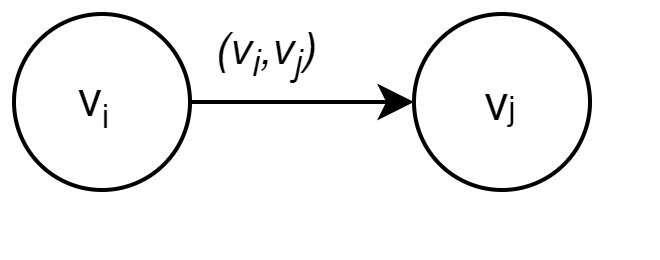
\includegraphics[scale=0.3]{figures/Multiagente/ex_grafo2.png}
    \label{fig:nos_arestas_grafos}
    \legend{Fonte: elaborada pelo autor.}
\end{figure}

Os graus de liberdade de entrada de um dado nó $v_i$ é definido como o número de vetores que a ponta da flecha se encontra em $v_i$. Do mesmo modo, os graus de liberdade de saída de um nó $v_i$ é dado pelo número de vetores que em $v_i$ se encontra a cauda da flecha.

Associado à cada aresta de um elemento em $E = (v_i, v_j)$ tem-se um peso $a_{ij} > 0$. O peso $a_{ij}$ representa a força de interação entre os nós $v_i$ e $v_j$. De modo que quanto maior o peso maior a influência tem o comportamento do agente $j$ sobre o agente $i$.
    %revisar esse parágrafo
Um grafo é dito bidirecional se e somente se $a_{ij} \neq 0$ e $a_{ji} \neq 0$, então tem-se que a comunicação entre agentes flui bidirecionalmente. Um grafo é dito unidirecional se $a_{ij} = a_{ji}$, para qualquer $i$ e $j$.


\section{Teoria algébrica dos grafos e consenso do controle cooperativo}

O controle cooperativo estuda a dinâmica de sistemas dinâmicos com múltiplos agentes com iterações um com o outro através de uma comunicação em grafo. 
O grafo representa as iterações e comunicações entre agentes. O objetivo do controle cooperativo é garantir a sincronia entre o comportamento e estados dos agentes, de modo que para cada agente só é disponível que as informações sejam entre o agente com os agentes vizinhos.

\subsection{Representação matricial dos grafos}
A estrutura e propriedade dos grafos podem ser estudadas examinando as propriedades de certas matrizes associadas. Dados os pesos $a{_ij}$ associados, o grafo pode ser representado pela \textbf{Matriz de Adjacência} ou conectividade $A = [a_{ij}]$, com $a_{ij}>0$ $se$ $(v_{j},v_{i}) \in E $ e $a_{ij}$ caso contrário.   
Define-se duas propriedades locais dos grafos, o graus de entrada e os graus de saída.
Os graus de entrada de um nó $v_{i}$ é definido pela equação \ref{eq:InDegree}, tal que $d_{i}$ é o somatório dos pesos $a_{ij}$ da linha $i$-th.
\begin{equation} \label{eq:InDegree}
   \hspace{6cm} % Adjust the value as needed
   d_{i} = \displaystyle\sum_{j=1}^{N}a_{ij}
\end{equation}

Os graus de saída de um nó $v_{i}$ é definido pela equação \ref{eq:OutDegree}, tal que $d_{i}$ é o somatório dos pesos $a_{ij}$ da coluna $i$-th.
\begin{equation}\label{eq:OutDegree}
\hspace{6cm} % Adjust the value as needed
    d_{i}^0 = \displaystyle\sum_{j = 1}^{N}a_{ji}
\end{equation}

Define-se duas propriedades globais dos grafos, o diâmetro do grafo , dada pela maior distância entre dois nós e o volume de entrada $(in)-volume$, dado pela soma dos nós de entrada
\begin{equation}
\hspace{6cm} % Adjust the value as needed
    VolG=\displaystyle\sum_{i}d_{i}
\end{equation}

\subsection{Matriz de Grafo Laplaciana}
Uma definição importante aplicada a sistemas multiagentes é a \textbf{Matriz Laplaciana}, que auxilia o estudo das propriedades da dinâmica do grafo de multiagentes. A mesma é obtida através da operação entre duas matrize, a Matriz Diagonal e a Matriz de Adjacência.
Define-se a matriz diagonal de graus de entrada, pela equação \ref{eq:matrizDiagonal}, em que para um agente $i$, tem-se o elemento $d_{i}$ como o somatório das flechas que apontam para o dado agente.
\begin{equation}\label{eq:matrizDiagonal}
\hspace{6cm} % Adjust the value as needed
    D = diag\{d_{i}\}
\end{equation}
Por fim a matriz Laplaciana $L$ é definida como $L = D-A$, tal que $D$ é a matriz Diagonal e $A$ é a matriz de Adjacência.
\\
Um exemplo de matriz laplaciana associada ao grafo pode ser ilustrada através da Figura \ref{fig:exemplo_grafo}, em que a matriz Diagonal $D$ é dada pela matriz \ref{eq:matriz_d1}. 

\begin{figure}
    \centering
    \caption{Exemplo de um grafo.}
    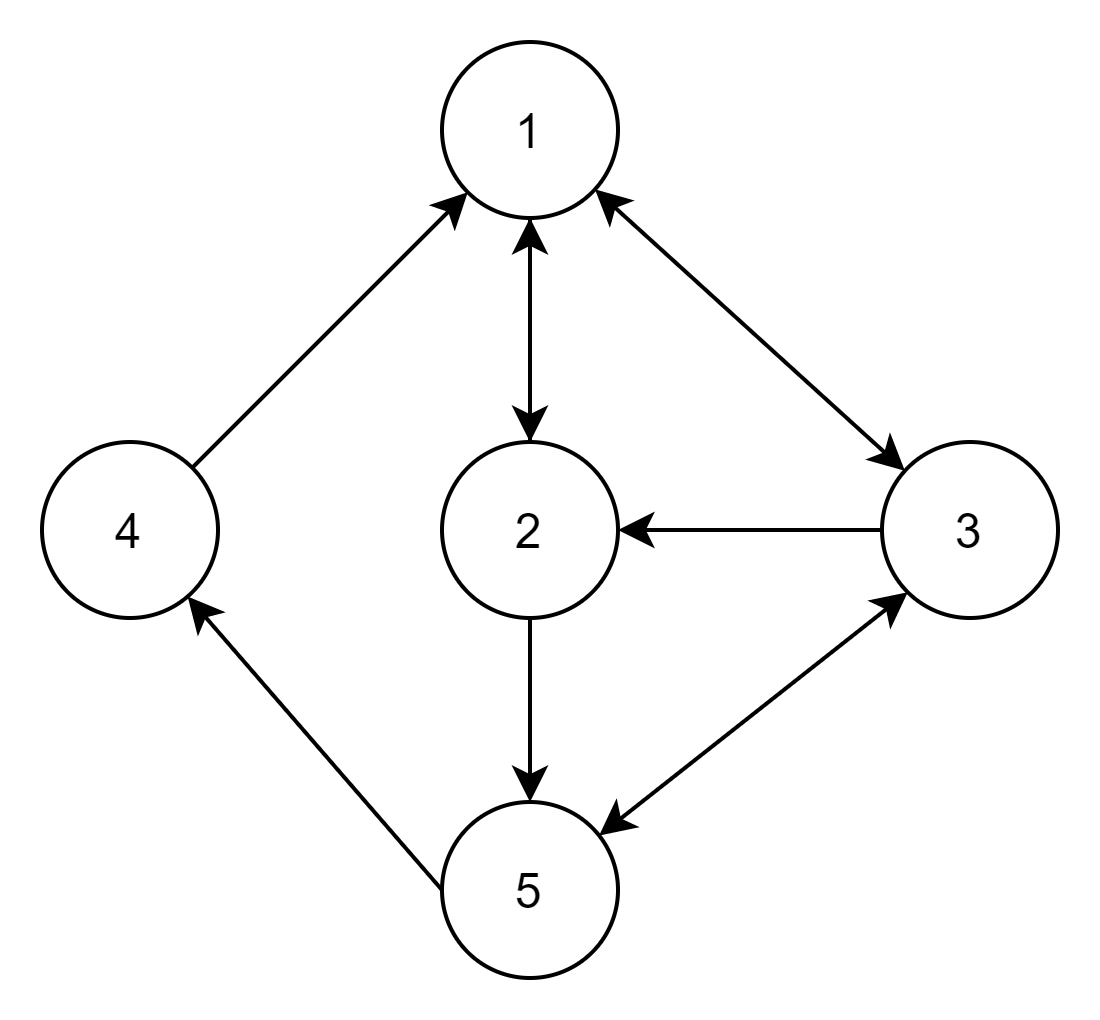
\includegraphics[scale=0.2]{figures/Multiagente/ex_grafos1.png}
    \legend{Fonte: elaborada pelo autor.}
    \label{fig:exemplo_grafo}
\end{figure}

\begin{equation}\label{eq:matriz_d1}
\hspace{6cm} % Adjust the value as needed
    D = \begin{bmatrix}
         3 & 0 & 0 & 0 & 0 \\ % graus de entrada do agente 1
         0 & 2 & 0 & 0 & 0 \\ % graus de entrada do agente 2
         0 & 0 & 2 & 0 & 0 \\ % graus de entrada do agente 3
         0 & 0 & 0 & 1 & 0 \\ % graus de entrada do agente 4
         0 & 0 & 0 & 0 & 2 \\ % graus de entrada do agente 5
    \end{bmatrix}
\end{equation}
A matriz A, dada pela Matriz de Adjacência \ref{eq:matriz_A1}.
\begin{equation}\label{eq:matriz_A1}
\hspace{6cm} % Adjust the value as needed
    A = \begin{bmatrix}
         0 & 1 & 1 & 0 & 0 \\ % conectividade do agente 1  
         1 & 0 & 0 & 0 & 1 \\ % conectividade do agente 2
         1 & 1 & 0 & 0 & 1 \\ % conectividade do agente 3 
         1 & 0 & 0 & 0 & 0 \\ % conectividade do agente 4 
         0 & 0 & 1 & 1 & 0 \\ % conectividade do agente 5 
    \end{bmatrix}
\end{equation}
Por fim, a matriz Laplaciana é dada por $L = D - A$.
\begin{equation}\label{eq:matriz_L1}
\hspace{1cm} % Adjust the value as needed
    L = \begin{bmatrix}
         3 & -1 & -1 & 0 & 0 \\ 
         -1 & 2 & 0 & 0 & -1 \\ 
         -1 & -1 & 2 & 0 & -1 \\ 
         -1 & 0 & 0 & 1 & 0 \\ 
         0 & 0 & -1 & -1 & 2 \\ 
    \end{bmatrix}
    = \begin{bmatrix}
         3 & 0 & 0 & 0 & 0 \\ % graus de entrada do agente 1
         0 & 2 & 0 & 0 & 0 \\ % graus de entrada do agente 2 
         0 & 0 & 2 & 0 & 0 \\ % graus de entrada do agente 3
         0 & 0 & 0 & 1 & 0 \\ % graus de entrada do agente 4
         0 & 0 & 0 & 0 & 2 \\ % graus de entrada do agente 5
    \end{bmatrix}
    - \begin{bmatrix}
         0 & 1 & 1 & 0 & 0 \\ % conectividade do agente 1  
         1 & 0 & 0 & 0 & 1 \\ % conectividade do agente 2
         1 & 1 & 0 & 0 & 1 \\ % conectividade do agente 3 
         1 & 0 & 0 & 0 & 0 \\ % conectividade do agente 4 
         0 & 0 & 1 & 1 & 0 \\ % conectividade do agente 5 
    \end{bmatrix}
\end{equation}


\section{Consenso com Integrador único}
Para o estudo inicial de controle cooperativo, tem-se a análise de um sistema multiagente formado por agentes $i$ com dinâmica dada por um integrador escalar único, modelada pela equação \ref{eq:int_Unico}
\begin{equation}\label{eq:int_Unico}
\hspace{6cm} % Adjust the value as needed
    \dot x_{i}  = u_{i} 
\end{equation}
com $x_{i}, u_{i} \in R $ . Isso corresponde que cada nó do grafo $G$, possui um agente com memória.

\subsection{Protocolo de controle distribuído para o consenso}
Para cada agente $i$, considere o protocolo de controle local dado pela equação \ref{eq:protocolo_controle_local}
\begin{equation}\label{eq:protocolo_controle_local}
\hspace{6cm} % Adjust the value as needed
    u_{i} = \sum\limits_{j \in N_{i}} a_{ij} (x_{j} - x_{i})
\end{equation}
com $a_{ij}$ sendo o peso de interação entre os estados dos agentes.Essa equação é conhecida como protocolo de votação local, em que o estado de cada agente depende tão somente do estado do agente vizinho, e a entrada de controle depende da da diferença dos estados em relação aos agentes vizinhos. De modo que percebe-se que se todos os estados forem os mesmo a entrada de controle tende a zero $\dot x_{i} = u_{i} = 0$.

Para a dinâmica de integrador único, é desejável que a equação \ref{eq:int_Unico}, resolva o problema de consenso, da dinâmica de malha fechada dada pela equação \ref{eq:consenso_Int_Unico}
\begin{equation}\label{eq:consenso_Int_Unico}
\hspace{6cm} % Adjust the value as needed
    \dot x_{i} = \sum\limits_{j \in N_{i}} a_{ij} (x_{j} - x_{i})
\end{equation}
Reorganizando a equação \ref{eq:consenso_Int_Unico}, tem-se que a equação. \ref{eq:consenso_Int_Unico_Expandido}
\begin{equation}\label{eq:consenso_Int_Unico_Expandido}
\hspace{6cm} % Adjust the value as needed
    \begin{split}
        \dot x_{i} &= -x_{i}\sum\limits_{j \in N_{i}} a_{ij} + 
        \sum\limits_{j \in N_{i}} a_{ij}x_{j} \\
        &= -d_{i}x_{i} + 
        \left[ a_{i1} \quad \cdots \quad a_{iN} \right] 
        \left[ x_{1} \, \vdots \, x_{N} \right]
    \end{split}
\end{equation}
tal que $d_{i}$ são os graus de liberdade, $x = [x_{1} \cdots x_{N}]$ $\in R^N$ o vetor de estados. Define-se a matriz $D$ como matriz diagonal formada por $D = diag \{d_{i}\}$, organiza-se a 
dinâmica global, através da matriz dada pela equação Laplaciana.
\begin{equation}
\label{eq:construcao_laplaciana}
\hspace{6cm} % Adjust the value as needed
    \begin{split}
        \dot x = -Dx +Ax &= -(D-A)x \\
        \dot x = u &= -Lx 
    \end{split}
\end{equation}
Através da equação \ref{eq:construcao_laplaciana}, e da matriz laplaciana de grafo tem-se que a dinâmica de malha fechada pode ser analisada através da matriz laplaciana dada.
Para a dinâmica de integrador único tem-se que se e somente se o grafo possui a topologia de spanning tree, então todos os estados dos nós vão a um valor de consenso dado por $x_{i} = x_{j} = c$. O valor de consenso é dado pela equação \ref{eq:valor_de_consenso}.
\begin{equation}\label{eq:valor_de_consenso} 
\hspace{6cm} % Adjust the value as needed
c = \sum\limits_{i = 1}^{N} p_{i}x_{i}(0)
\end{equation}
tal que $w_{1} = [p_{1} \cdots p_{N}]^{T}$, é o vetor normalizado pela esquerda da matriz laplaciana $L$, para $  \lambda_{1} = 0$. De modo que a constante de tempo é dada por \ref{eq:const_tempo} e $\lambda_{2}$ sendo o segundo autovalor da matriz L.
\begin{equation}\label{eq:const_tempo}
\hspace{6cm} % Adjust the value as needed
   \tau = 1 / \lambda_{2}
\end{equation}


\subsection{Consenso com líder}
\label{sub:consenso_lider}
Um "(directed) tree" é um um grafo onde todo nó exceto um é chamado de líder, e possui grau de entrada unitário. De modo que todos os outros nós possuem um consenso liderado pelas condições iniciais do líder.
O valor de consenso é dado pela equação \ref{eq:valor_de_consenso}, de modo que $p_{i}$ é o $i-{th}$ componente para o autovetor pela esquerda de $w_{i}$ para $\lambda_{1} = 0$, tal consenso é na verdade a média ponderada das condições iniciais das raízes dos nós ou do líder em um grafo. 
%% Adicionar simulação parecida com a simulação da pág 42 do livro, sobre consenso com líder.

\subsection{Consenso para nós com estados como vetores}
Nas condições de integrador único e integrado duplo apresentadas anteriormente os estados são tidos como escalares, para os exemplos em que os estados são vetores tais como $x_{i}, u_{i} \in R^{N}$ tem-se que os vetores globais de estados e controle são respectivamente $x = [x_{1}^{T} \cdots x_{N}^{T}]^{T} \in R^{nN} , 
u = [u_{1}^{T}  \cdots u_{N}^{T}]^{T} \in R^{nN} $ e os elementos dados pelos pesos de consenso $a_{ij}$ e a diagonal $d_{i}$ são multiplicados pela matriz identidade $I_{n}$, de modo que a dinâmica global do sistema é dada pela equação \ref{eq:consenso_vetorial}

\begin{equation}\label{eq:consenso_vetorial}
 \begin{aligned}
 \hspace{6cm} % Adjust the value as needed
    u = -(L \otimes I_{N})x \\
    \dot x = -(L \otimes I_{N}) x
    \end{aligned}
\end{equation}
dado que $\otimes$ é definido como produto de kronecker.

%\subsection{Movimento invariante para consenso de primeira ordem}
Para o protocolo de primeira ordem local dado por %\ref{eq:construcao_laplaciana} foi garantido que para a topologia de $spannig tree$ o consenso é alcançado. 


% Falta as  associações com as referências no capítulo 2.


\chapter{Redes de Petri}
\label{chap:petri}

\section{Modelagem de Sistemas}
Para a modelagem de sistemas é importante entender as principais características do sistema que está sendo estudado, no propósito de uma revisão na classificação de sistemas,foi elencado em \cite{cassandras} tais classificações, observe que elas não são necessariamente auto exclusivas: 

\textbf{Sistema Dinâmico e Estático:}  Em sistema estático a saída é sempre independente dos valores de entrada passados, já em um sistema dinâmico os valores de saída dependem dos valores anteriores da entrada. Equações diferencias ou a diferença são geralmente requeridas para representar o comportamento de sistemas dinâmicos.

\textbf{Sistema Variante e Invariante no Tempo:} Em um sistema invariante no tempo o comportamento do mesmo não se altera com o passar do tempo. Tal sistema é dado com estacionário pois se aplicada a mesma entrada ao longo do tempo o sistema responderá com o mesmo comportamento.

\textbf{Sistemas Lineares e Não Lineares: } Um sistema linear obedece a condição $g(a_1u_1 + a_2u_2) = a_1g(u_1) + a_2g(u_2)$ tais que $u_1$ e $u_2$ são dois vetores de entrada, $a_1$ e $a_2$ dois números reais e $g(.)$ é a saída resultante. 

\textbf{Sistema em Estado Contínuo e Discreto: } Um sistema contínuo pode ter a variável de estado representa por um número real ou complexo, já o sistema discreto é representado por uma série de elementos discretos.

\textbf{Sistema Orientado a Eventos e Tempo: } Em um sistema orientado ao tempo o estado do sistema muda com a mudança de tempo, já a eventos a mudança de estado ocorre de forma instantânea a partir da ocorrência de um evento.

\textbf{Sistema Determinístico e Estocástico: } Um sistema se torna estocástico quando possui uma ou mais de uma variável estocástica. Nesse caso o estado do sistema é descrito por um processo estocástico.

\textbf{Sistema em Tempo Contínuo e Discreto: } Um sistema em tempo contínuo possui todas as entradas definidas para todos os valores de tempo possíveis. 

No escopo do trabalho proposto o a modelagem em redes de petri é utilizada para um sistema a eventos discretos seguindo a seguinte árvore de escopos dada pela figura \ref{fig:arvore_escopo}
\begin{figure}
    \centering
    \caption{Árvore de escopo de um sistema a eventos discretos.}
    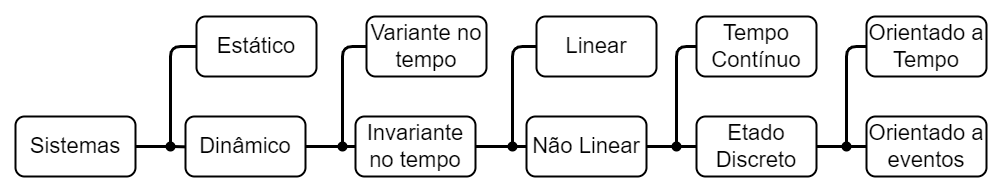
\includegraphics[scale=0.4]{figures/Petri/arvore_escopo.png}
    \legend{Fonte: adaptado de \cite{cassandras}. }
    \label{fig:arvore_escopo}
\end{figure}

  % \centering
  %   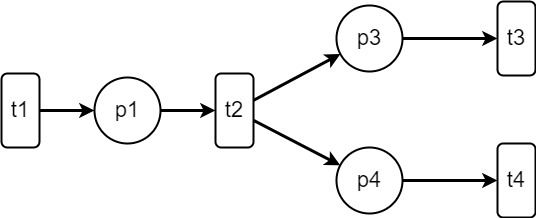
\includegraphics[scale=0.4]{figures/Petri/paralelismo_sincrono.jpg}
  %   \caption{Exemplo paralelismo Síncrono} 
  %   \label{fig:paralelismo_sincrono}
    
\subsection{Modelagem de sistemas a eventos discretos}

Em si tratando da modelagem de sistemas a eventos discretos tem-se três elementos principais utilizados na modelagem eventos(instantes e mudanças de estados), atividades(evolução do sistema físico entre dois eventos) e processos (sequência de eventos e atividades no sistema). 

Na evolução dos processos no sistema os processos podem ocorrer de forma totalmente independente entre si, enquanto outras atividades necessitam de uma determinada sincronização ou até uma sequência de eventos prévios. Uma forma de diferenciação de interações entre processos é apresentada por \cite{vallete}, como:

\textbf{Cooperação:} Os processos convergem para um objetivo comum, de modo que anteriormente há uma relativa independência antes do ponto de sincronização.

\textbf{Competição:} Os processos necessitam de um dado recurso, caso esse recurso seja abundante para todos os processos, dados processos poderiam ser descritos de forma independente, caso contrário faz-se necessário o compartilhamento de recursos envolvendo uma exclusão mútua a partir de um ponto de sincronização.

\textbf{Pseudo-Paralelismo:} O paralelismo é apenas aparente e os eventos por mais que sejam independentes nunca serão simultâneos pois são acionados por um relógio comum, a exemplo de um sistema operacional que por mais que processe várias tarefas, porém o processador só processa um ciclo de instrução por vez.

\textbf{Paralelismo Verdadeiro:} Os eventos podem ocorrer de forma simultânea, não existindo uma escala de tempo em comum, a exemplo de vários processadores operando tarefas distintas.

\section{Representação em máquina de estados}
Uma das representações mais clássicas para modelagem de sistemas à eventos discretos é a máquina de estados, para o caso de uma número de estados finitos enumera-se os possíveis estados e descreve-se os eventos referente as mudanças de estado, descrevendo-se assim cada estado a a partir do estado anterior.

O modelo matemático para a máquina de estado finita é dada a partir da equação \ref*{eq:finit_state_machine_equation}, em que $E$ é um conjunto finito de estados, dado pelo estado inicial $E_0$, um alfabeto de entrada $A$, e uma função de transição de estados $\theta$, dado por $\theta : E \times A \rightarrow E$, associando cada par de estado-entrada ao próximo estado.

\begin{equation}\label{eq:finit_state_machine_equation}
\hspace{6cm} % Adjust the value as needed
    M = (E; A; \theta; E_0)
\end{equation}
De acordo com \cite{vallete} este modelo explicita a noção de eventos e parcialmente a de atividade, não explicitando, entretanto, a noção do processo com as evoluções simultâneas de diversos processos paralelos, de modo que uma máquina de estado finita descreve apenas um único processo sequencial.

\subsection{Modelagem de processos sequenciais}
Para a descrição de vários processos sequências, uma das soluções é representar o sistema por um conjunto de máquinas de estados finitos. Quando as máquinas de estados são independentes, esse modelo se aplica sem dificuldade, porém quando existe competição ou cooperação entre os processos faz-se necessário o uso de processos sequenciais comunicantes. A sincronização é descrita através da intervenção na função de transição de estados $\theta$ de uma máquina.

\subsubsection{Representação com refinamentos sucesssivos}
Um dos contrapontos dessa abordagem é que independente do método utilizado, a representação das comunicações entre as máquinas é diferente da representação interna da sequência de uma máquina. Portanto, tal abordagem não é compatível com a abordagem top-down de refinamento sucessivos. É necessário desde do início da modelagem a escolha de uma decomposição que não será colocada em causa a posteriori. 

\subsubsection{Explosão combinatória}
Outro ponto de análise dessa forma de modelagem é que para cada informação partilhada entre as máquina ou troca de sinais entre as máquinas é necessário analisar o comportamento global do sistema através do recálculo de uma nova máquina de estado que descreva o sistema de forma global. Neste caso, ocorre a problemática da explosão combinatória do número de estados definida pela relação entre $k$ máquinas e $n$ estados, produzindo uma máquina de $n^k $ estados, ocorrendo uma explosão combinatória a medida que k e n aumentam.

\subsubsection{Não-independência de submáquinas e bloqueio}
Em se tratando de sistemas com paralelismo um dos problemas comuns que podem acontecer é o de bloqueio (\textit{dead-lock}) em que a máquina de estado não consegue evoluir pois depende da transição de um estado de outra máquina que por sua vez encontra-se igualmente no mesmo estado de espera. Existem técnicas na teoria de máquinas de estados finitos que evitam o bloqueio, porém a estrutura do sistema acaba sendo comprometida, perdendo assim a representativa clara do sistema e suas transições.

\section{Modelagem utilizando Rede de Petri}
As redes de Petri também são uma ferramenta de modelagem inicial para o algoritmo de programação com ferramentas intrínsecas que analisam o algoritmo para evitar que o sistema entre em exceções,(LEE et al., 2006). 
De acordo com (GIUA; SILVA, 2017), as redes de Petri têm sido consideradas com um modelo adequado para um controle supervisório com o objetivo de abranger uma grande classe de problemas e explorar a análise algébrica necessária para otimização. Tratando-se também da análise para a planta não alcançar determinadas marcações indesejadas;

A utilização de redes de petri como camada de abstração para tomada de decisões, escolha de estratégias diante dos problemas e organização dos agentes para seguir um determinado plano foi trabalhada como framework por (EBADI et al., 2010), em que todo o processo de mais alto nível de decisão foi modelado para a rede de petri. Nesse presente trabalho além da abstração pela rede de petri como tomada de decisão também é apresentando o algoritmo de consenso como solução do problema de controle e cooperação entre os agentes dada uma tomada de decisão de organização dos grupos.

A descrição dos eventos e transições do sistema é dada através da rede de petri pelos lugares, fichas e transições, para representar os "estados" do sistema são utilizados os lugares, já as transições movimentam os recursos, ou seja, as fichas de um lugar para outro, dada a condição que a transição só possa ser disparada caso os lugares a ela ligada estejam completas com os recursos requisitados, fazendo assim interdependências em que um determinado estado só pode ser alcançado caso determinadas condições satisfeitas.

O comportamento dinâmico do sistema se dá através do disparo das transições, evento que faz com que o sistema passe do estado atual para o próximo estado. Tal disparo consiste em duas etapas, a primeira de retirar as fichas dos lugares de entrada e por fim depositar as fichas em cada lugar de saída.

\subsection{Evolução síncrona e assíncrona}
A rede de petri pode representar sistemas com eventos síncronos e assíncronos, em que são necessários momento de espera para acontecer determinados eventos assim como a independência de eventos que podem ou não ocorrer de forma simultânea.

Observa-se na figura \ref{fig:paralelismo_sincrono} um evento caracterizado como divisão em que no disparo da transição $t_2$ uma ficha é retirada de $p_1$ e simultaneamente é colocada uma ficha em $p_3$ e $p_4$ daí em diante a evolução do sistema ocorre de forma assíncrona podendo ou não haver disparos concorrentes.  

\begin{figure}[ht]
    \centering
    \caption{Exemplo paralelismo Síncrono.}
    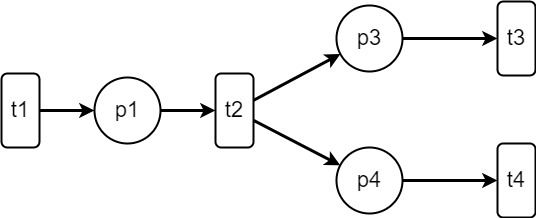
\includegraphics[scale=0.4]{figures/Petri/paralelismo_sincrono.jpg}
    \legend{Fonte: Elaborado pelo autor.}
    \label{fig:paralelismo_sincrono}
\end{figure}

Observa-se na figura \ref{fig:paralelismo_assincrono} um evento caracterizado como junção em que para haver o disparo de $t_3$ é necessário que haja uma ficha tanto em $p_3$ quanto em $p_4$, o consumo dessas fichas ocorre de forma síncrona tal evento implica necessariamente de uma espera em que ou $p_3$ espera a chegada do recurso em $p_4$ ou o contrário, garantindo assim que $p_5$ só receba uma fica quando essas duas condições forem satisfeitas. Antes do disparo de $t_3$ o sistema pode evoluir de forma assíncrona com disparos independentes de $t_1$ e $t_2$.

\begin{figure}[ht]
    \centering
    \caption{Exemplo paralelismo Assíncrono.}
    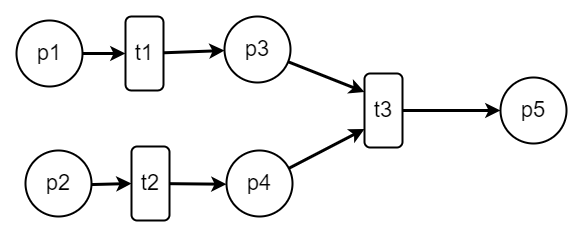
\includegraphics[scale=0.4]{figures/Petri/paralelismo_assincrono.png}
    \legend{Fonte: Elaborado pelo autor.}
    \label{fig:paralelismo_assincrono}
\end{figure}


\subsection{Caminhos alternativos e Repetição}
Um evento que também pode ser modelado são o de caminhos alternativos e variações de sequência de disparos em uma rede de petri, em que em determinado momento na rede há um lugar ligado a entrada de uma ou mais transições, ocorrendo assim a sensibilização de tais transições, podendo ocorrer portanto o disparo de qualquer uma das transições, tomando-se assim um caminho alternativo caso outra transição fosse disparada.

Observa-se esse fenômeno na modelagem descrita pela figura \ref{fig:caminhos_alternativos}, em que no momento em que $p_1$ recebe uma ficha é sensibilizada as transições $t_1$ e $t_2$, de modo que a rede de petri não restringe a escolha de um ou outra transição, porém caso uma transição seja disparada a outra não poderá ser, ocorrendo assim uma competição pelo recurso em que a transição que disparar primeiro recebe o recurso. Dado a ocorrência da repetição da rede através de $t_5$, novamente a tomada de decisão entre $t_1$ e $t_2$ ocorrera, podendo assim ocorrer um caminho alternativo ao caminho prévio dada a sequência de disparo ocorrida.

A figura \ref{fig:caminhos_alternativos}, também modela um evento de repetição através da transição $t_5$, em que dada a chegada da ficha no lugar $p_5$ tal ficha pode retornar ao lugar de origem $p_1$ ocorrendo assim o restabelecimento da rede e infinitas repetições.

\begin{figure}[ht]
    \centering
    \caption{Exemplo de Caminhos alternativos e Repetição.}
    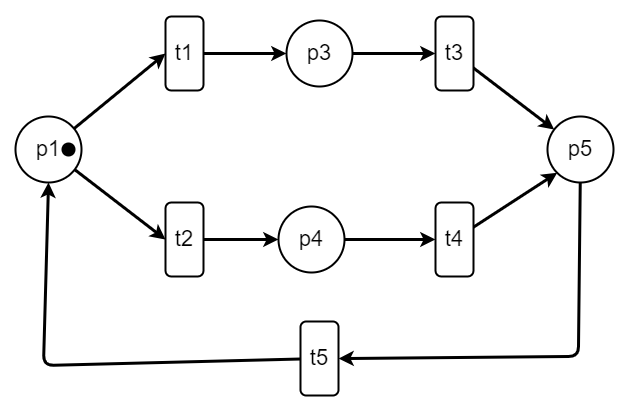
\includegraphics[scale=0.4]{figures/Petri/caminhos_alternativos.png}
    \legend{Fonte: Elaborado pelo autor.}
    \label{fig:caminhos_alternativos}
\end{figure}

\section{Redes de Petri}
A rede de Petri é uma ferramenta gráfica e matemática para modelagem e controle de sistemas à eventos discretos, dado que o sistema a ser escolhido é um sistema que pode ser modelado através de tal ferramenta, com o intuito de obter uma visualização gráfica do processo, implementar lógica de controle e sincronismo, analisar propriedades da rede entre outras.
Para a modelagem proposta utilizou-se a ferramenta do CPN Tools, assim como as funcionalidades envolvendo hierarquia para maior legibilidade da rede.

De acordo com \cite{cassandras}, os eventos na Rede de Petri \gls{RP} são relacionados as transições, de modo que para que aconteça o disparo de uma transição é necessário satisfazer determinadas condições inscritas na rede.
As informações relacionadas a tais condições estão contidas em lugares, que são vistos como "entradas" das transições. Lugares, transições e as relações entre eles são os componentes básicos de uma RP. A RP possuí dois tipos de nós, lugares e transições, e os arcos que conectam eles. Na definição de grafos a RP é classificada com um grafo bipartido de modo que os arcos não podem conectar diretamente dois nós do mesmo tipo, exemplo lugar a lugar ou transição a transição.
A definição de grafo é dada a seguir.

\subsection{Linguagem Formal}
De acordo com \cite{peterson}, a Rede de Petri é definida como um grafo bipartido ponderado, dado pelo conjunto $(P,T,A,w,x)$, tal que:
\begin{itemize}
    \item $P$ é o conjunto finito de lugares (um tipo de nó na grafo)
    \item $T$ é o conjunto finito de transições (o outro tipo de nó no grafo)
    \item $A \subseteq (P \times T) \cup (T \times P)$ é o conjunto de arcos dos lugares para as transições e das transições para os lugares no grafo.
    \item  $w : A \rightarrow \{1, 2, 3, \ldots\}$ são as funções de ponderação dos arcos.
    \item $x$ : é a marcação da rede de Petri dada pela função $x : P \rightarrow \mathbb{N} = \{0, 1, 2, \ldots\}$, tal marcação é definida como um vetor linha $x = x(p_1), x(p_2), ..., x(p_n)$, tal que $n$, é o número de lugares na rede.
\end{itemize}
É considerado que em $(P,T,A,w)$, não tem lugares em transições isolados.
Na representação em grafos os lugares $P = \{p_1,p_2,p_3, ..\}$ são representados com um círculo, as transições $T = \{t_1,t_2,t_3,...\}$ como retângulos. Os conjunto de arcos $A = \{w_1,w_2,w_3,...\}$, cada arco $w$ é representado em função de um lugar e uma transição e o peso associado como $w_k= (p_i,t_j) = W$ , tal que o arco liga o lugar $p_i$ a transição $t_j$ e possui o peso igual a $W$. A marcação no grafo é dada como fichas (ponto preto) no lugar marcado $p_i$ tal que $x(p_i) \in \mathbb{N}$.

Um exemplo de rede com os elementos citados é representado pelo grafo na figura \ref{fig:ex_rp}. Os lugares da rede de petri são  representados pelos círculos $P = \{p_1,p_2,p_3 .. p_7\}$, as transições $T=\{t_1, t_2 ,.., t_5\}$, já no caso das transições o conjunto $W$ é definido da seguinte forma:
$W = \{w_1,w_2, .. w_8 \}$
onde:
\begin{itemize}
     \item $w_1 = (p_1, t_1)$ representa um arco que sai de $p_1$ e entra em $t_1$.
    \item $w_2 = (t_1, p_3)$ representa um arco que sai de $t_1$ e entra em $p_3$.
    \item $w_3 = (t_1, p_2)$ representa um arco que sai de $t_1$ e entra em $p_2$.
    \item $w_4 = (p_2, t_3) = 2$ representa um arco que sai de $p_2$ e chega em $t_3$ com peso igual a $2$.
    \item $w_5 = (p_3, t_4)$ representa um arco que sai de $p_3$ e entra em $t_4$.
    \item $w_6 = (t_4, p_5)$ representa um arco que sai de $t_4$ e entra em $p_5$.
    \item $w_7 = (p_5, t_3)$ representa um arco que sai de $p_5$ e entra em $t_3$.
    \item $w_8 = (t_3, p_4)$ representa um arco que sai de $t_3$ e entra em $p_4$.
Por fim, a representação da marcação tem-se que no lugar $p_1$ a quantidade de 1 ficha e nos outros nenhum ficha, formando o vetor linha representado na equação \ref{eq:initial_mark_example}:
\begin{equation}
\label{eq:initial_mark_example}
\hspace{6cm} % Adjust the value as needed
    \begin{split}
    X &= [x(p_1), x(p_2), .., x(p_5)] \\
    &= [1,0,0,0,0]           
    \end{split}
\end{equation}

\end{itemize}
\begin{figure}[ht]
\centering
\caption{Exemplo de Rede de Petri.}
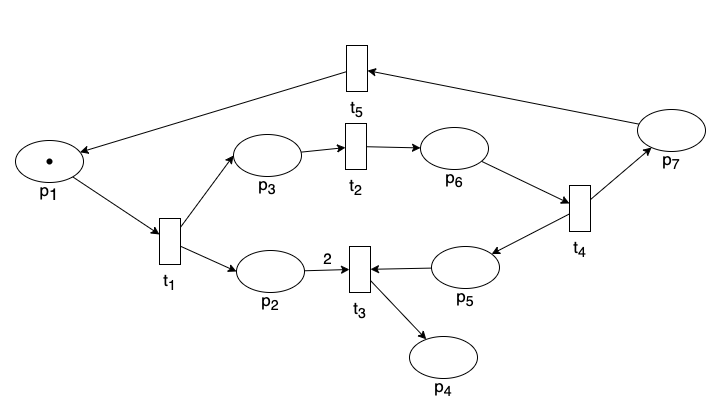
\includegraphics[scale=0.8] {figures/Petri/exemplo_rp.png}
\label{fig:ex_rp}
\legend{Fonte: Elaborado pelo autor.}
\end{figure}

\subsection{Redes de Petri Colorida}
A rede apresentada anteriormente com elementos simples de arcos, marcações, transições, de acordo com \cite{jensen} são denominadas de redes de Petri de baixo nível, geralmente utilizadas para modelagem de hardware, já para a modelagem de sistemas com concorrência, comunicação, hierarquia. Exemplo  sistemas de manufatura, sistemas baseados em agentes, pode-se utilizar as redes de Petri de alto nível, também denominadas como redes de Petri colorida. 

As redes de Petri  coloridas (\gls{RPC}) são uma ferramenta gráfica e matemática que se adaptam bem a um grande numero de aplicações, tais como protocolos de comunicação, controle de oficinas de fabricação. É uma combinação das redes de Petri com linguagem de computação. Os elementos da \gls{RPC} são baseados em hierarquias, que permite que módulos tenham submódulos, permitindo a reusabilidade dos módulos. Isso permite trabalhar tanto com a abordagem \textit{top-down}, quanto \textit{bottom-up}, na construção dos modelos em RPC, capturando assim diferentes camadas de abstração na modelagem do sistema.

%% Apresentar em formato de quadro.
\chapter{Simulação}
\label{chap:simulation}
Nessa seção, busca-se validar a abordagem integrada de Modelagem por meio de Redes de Petri Coloridas (RPC) e Controle Cooperativo. Para realizar essa validação, optou-se por empregar a estratégia de simulação, utilizando um sistema multiagente composto por diversos componentes, os quais foram concebidos para representar um ambiente similar a um sistema industrial.

Neste processo de simulação, são utilizadas ferramentas de software dedicadas à modelagem em RPC, com destaque para o CPN-Tools.\footnote{pode ser acessada em \texttt{https://cpntools.org/}} Essa ferramenta oferece funcionalidades específicas para a edição, simulação e análise de Redes de Petri Coloridas. A escolha do CPN-Tools visa proporcionar uma representação fiel e detalhada do sistema em estudo.

Para a implementação do algoritmo matemático de consenso, optou-se por utilizar a linguagem de programação Python. Essa escolha deve-se à reputação da linguagem como sendo de alto nível, funcional e orientada a objetos, oferecendo assim uma abordagem versátil e eficiente para a execução do algoritmo em questão.

Ao unir a simulação do sistema multiagente com as capacidades do CPN-Tools e a flexibilidade do Python, almeja-se obter resultados robustos que validem a eficácia da abordagem proposta. Esta seção detalhará o processo de simulação, desde a definição dos parâmetros até a análise crítica dos resultados obtidos, proporcionando uma compreensão clara e abrangente da validade e desempenho da abordagem integrada.

\section{Planta Industrial}
A gestão de vagões em uma planta industrial, que permite a ultrapassagem entre eles por meio de mudanças nas pistas, representa uma abordagem inovadora no contexto ferroviário industrial. Esse sistema dinâmico busca otimizar o movimento e a alocação de vagões, proporcionando flexibilidade e eficiência operacional.

Ao incorporar a capacidade de ultrapassagem, a planta industrial adquire versatilidade, possibilitando a reorganização estratégica dos vagões para atender a demandas específicas. Essa funcionalidade torna-se particularmente valiosa em situações onde é necessário priorizar determinados vagões, reduzir tempos de espera ou melhorar o desempenho global do sistema ferroviário dentro do contexto da planta industrial.

A implementação de mudanças nas pistas como um meio de permitir a ultrapassagem requer uma coordenação precisa e um controle eficaz do sistema. Técnicas como Redes de Petri Coloridas (RPC) ou algoritmos de controle cooperativo podem ser empregados para modelar e simular o comportamento dinâmico da planta, considerando as interações entre os vagões e as mudanças nas pistas.

Um exemplo de representação desse sistema escolhido é demonstrada na figura \ref{fig:pista_com_dois_agentes}, tal que:
\begin{itemize}
    \item Os componentes $L_1$ e $L_2$ ilustrados em formato triangular são os vagões que representam os dois autômatos, ou agentes do sistema.
    \item As curvas $d_1,d_2,..,d_6$ representam as pistas pelas quais os vagões se locomovem, de modo os dois vagões estão posicionados incialmente na pista denominada de $d_1$.
    \item os elementos $x_1,x_2,x_3,x_4$ representam as quatro chaves responsáveis por fazer a mudança de via, elas podem comutar em duas posições diferentes a posição $b$ que representa o caminho de menor comprimento ou a posição $a$ que representa o caminho de maior comprimento.
\end{itemize}

\begin{figure}[h]
\centering
\caption{Planta com pista, vagões e pontos de mudança de via }
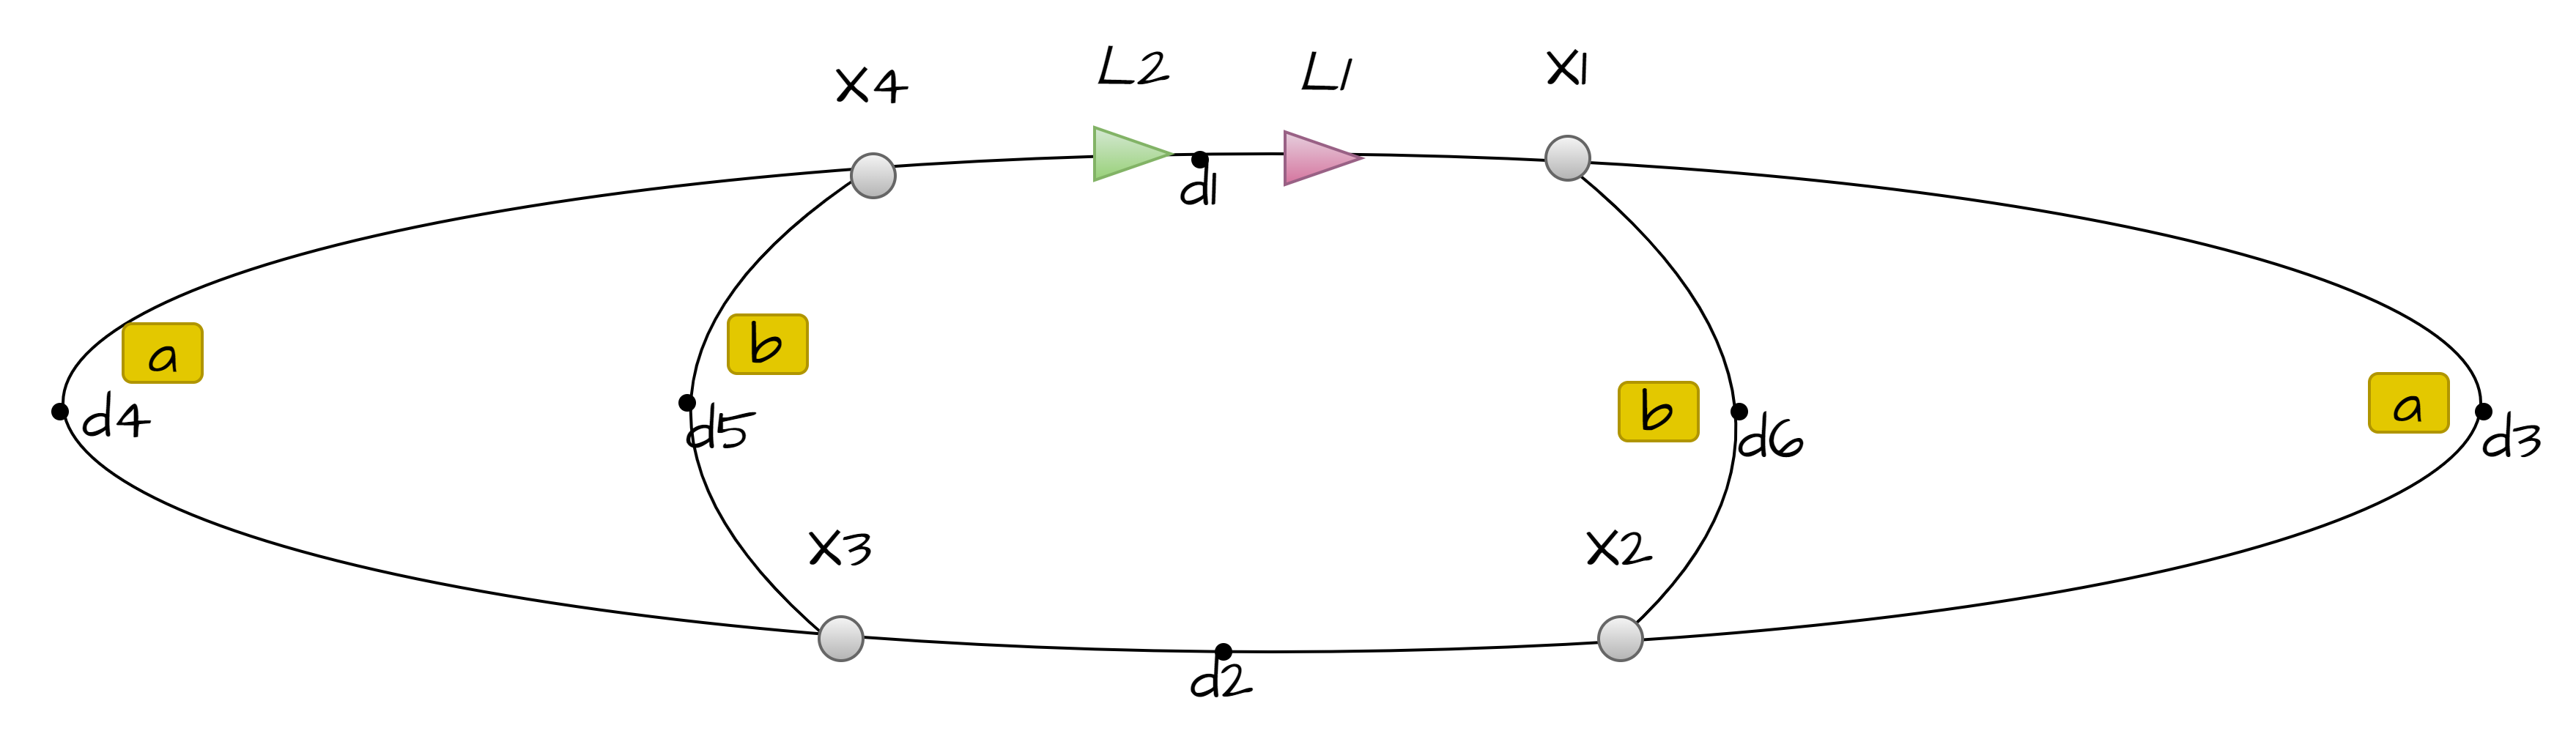
\includegraphics[width=1\linewidth]{figures/Simulation/Planta/planta_dois_agentes.png}
\label{fig:pista_com_dois_agentes}
\legend{Fonte: Elaborado pelo autor.}
\end{figure}

Para a simulação específica, os vagões movem-se entre pistas, e para efetuar uma ultrapassagem, é necessário que o vagão a ser ultrapassado siga pelo caminho mais longo, enquanto o vagão ultrapassante escolhe o caminho mais curto.

A chave de ultrapassagem foi designada como $x_1$. Quando o comando de ultrapassagem é acionado, inicialmente a chave se move para a posição $a$, assegurando o desvio para a pista mais longa. Em seguida, ela se move para a posição $b$, garantindo o desvio para a pista mais curta.

A chave $x_2$ desempenha o papel de primeiro desviar para a posição $b$, para receber o vagão da pista $d_6$. Posteriormente, comuta para a posição $a$, para receber o vagão da pista $d_3$.

As chaves $x_3$ e $x_4$ permanecem fixas na posição $b$, assegurando o percurso mais curto. Esse arranjo permite uma ultrapassagem de vagões de forma segura e otimizada entre as pistas.

\section{Modelagem em Redes de Petri Colorida}
\label{sec:model_RPC}
Para a modelagem do sistema proposto em Redes de Petri Colorida, foi definido o seguinte conjunto de cores para representar o tipo de token que vai ser alocado nos lugares da RPC de acordo com o seguinte quadro \ref{qua:conj_cores}.

\begin{quadro}[h]
\centering
\caption{Conjunto de Cores na RPC}
\begin{tabularx}{\textwidth}{|c|c|X|X|}
\hline
\textbf{Nomenclatura} & \textbf{Tipo}    & \textbf{Comando}                             & \textbf{Descrição} \\
\cline{1-4}
D & Inteiro & \texttt{colset D = int;} 
& Conjunto que indica a sequência dos vagões, onde o número 1 representa o vagão à frente, o número 2 representa o vagão atrás do 1, e assim por diante. \\ 
\cline{1-4}
X & String  & \texttt{colset X = string;} 
& Conjunto que representa a posição em que a chave se encontra, exemplo "a" para a posição A e "b" para a posição B. \\
\cline{1-4}
L & String  & \texttt{colset L = string;}         
& Conjunto de cores que representa os vagões ao longo da pista em que "L\_1" é o vagão L1 e "L\_2" o vagão L2. \\
\cline{1-4}
Ord & Record  & \texttt{colset Ord = record seq:D * train:L;} 
& Conjunto de cores que representa a associação do vagão L com a posição D,
de modo que caso "L1" esteja na primeira posição, será representado por "seq:1,train:L1". \\ 
\cline{1-4}

\end{tabularx}
\legend{Fonte: Elaborado pelo autor.}
\label{qua:conj_cores}
\end{quadro}

 Para cada conjunto de cores foi definido as variáveis correspondentes que serão alocados na inscrição dos arcos ao longo da RPC, de acordo com o quadro \ref{qua:variaveis_RPC}.

\begin{quadro}[ht]
\caption{Conjunto de Variáveis na RPC}
\begin{tabularx}{\textwidth}{|c|c|c|X|}
\cline{1-4}
% Cabeçalho
\textbf{Variável} & \textbf{Tipo} & \textbf{Exemplo} & \textbf{Descrição} \\ 
\cline{1-4} % Linha 1
d & D & 1`(1) ou 1`(2) & Variável de tipo Inteira, no exemplo tem-se 1 ficha com o valor 1, ou 2 fichas com valor 1, mais uma ficha com valor 2 \\ \cline{1-4} % Linha 2
x & X & 1`("a") ou 1`("b") & Variável do Tipo \textit{String} referente a posição de chave, pode ser do tipo "a" ou do tipo "b",como no exemplo. \\ \cline{1-4} % Linha 3
l & L & 1`("l1") ou 1`("l2") & Variável do Tipo \textit{String} referente ao vagão/trem que nos casos podem ser do tipo "l1" ou "l2", como no exemplo para dois agentes \\ \cline{1-4} % Linha 4
ord & Ord & 1`\{seq=2,train="l1"\} & Variável do Tipo \textit{record seq:d * train:L}, no exemplo descrito indica que o trem "l1" está na posição 2. \\ \cline{1-4} 
\end{tabularx}
\label{qua:variaveis_RPC}
\legend{Fonte:Elaborado pelo Autor}
\end{quadro}

Para a abstração e melhor organização e legibilidade da representação na RPC, foram definidos dois níveis hierárquico o nível mais acima da Pista, e o nível mais abaixo o de controle e comando. Cada nível possui um conjunto de módulos que podem ser agrupados em 3 principais funcionalidades, Pista, Controle das Chaves "X" e controle de Ordenação dos vagões "L", como demonstrado na figura \ref{fig:hierarquia_RPC}. Observa-se que para o controle das chaves X, foi definido 4 módulos de controle 1 para cada chave, que são responsáveis por gerenciar em qual posição cada respectiva chave irá estar. No caso do componente de Controle de Ordenação foram definidos 2 módulos, o de "Ordem", responsável por gerar o comando de "Ultrapassagem" ou "Não Ultrapassagem", já o módulo de "Inverter Ordem" é responsável por atualizar as ordem do vagões através da leitura da pista.

\begin{figure}[ht]
    \centering
    \caption{Modelo dos Componentes Hierárquicos da RPC}
    \label{fig:hierarquia_RPC}
    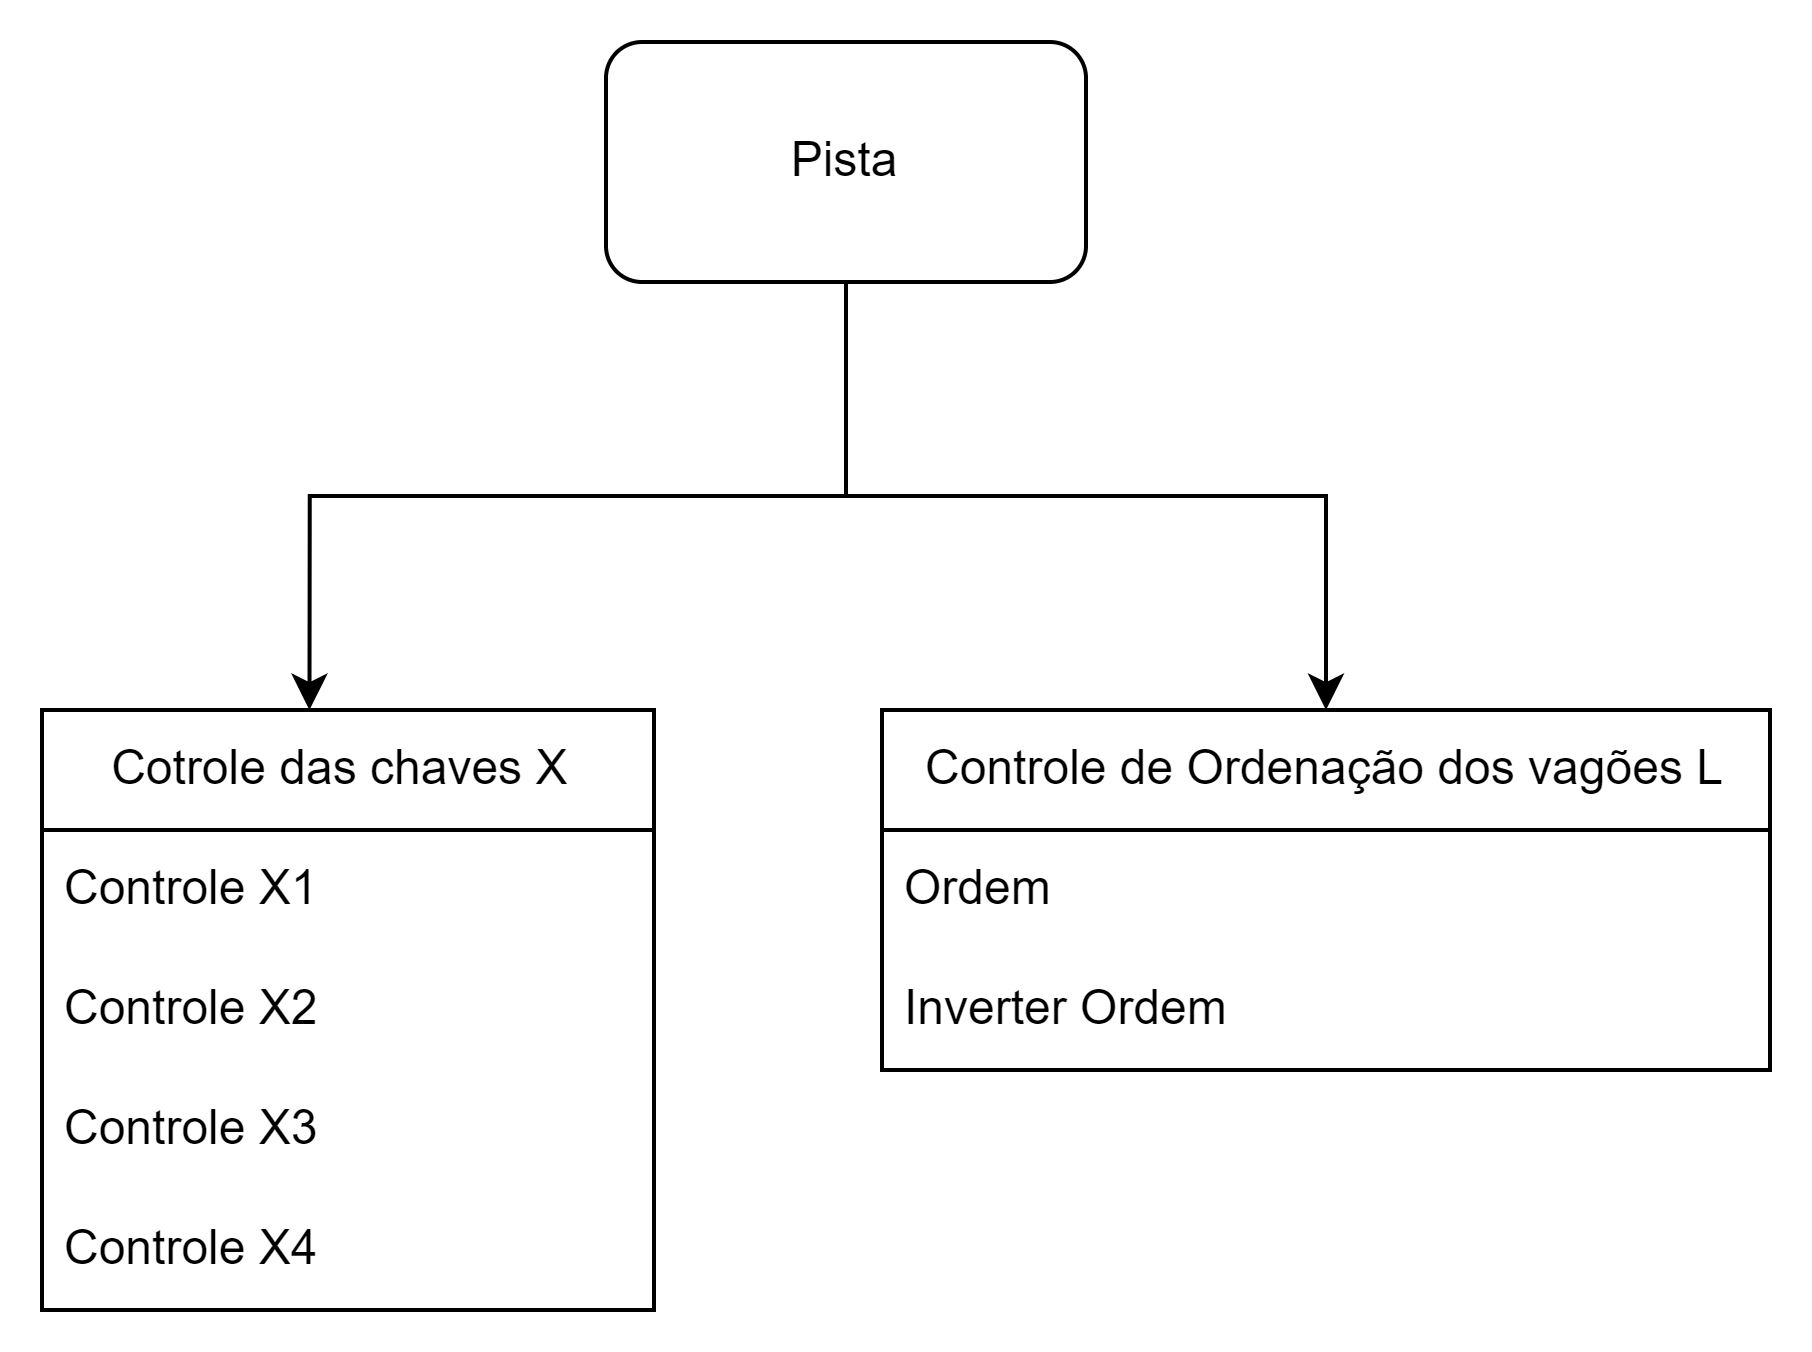
\includegraphics[width=0.8\linewidth]{figures//Simulation//Modelagem/hierarquia.png}
    \legend{Fonte: Elaborado pelo autor.}
\end{figure}

A RPC de camada superior é dada pela figura \ref{fig:rede_geral}, nela é possível verifica a existência de outras sub-redes dada pelas transições \textit{Controle} $X_1$ a $X_4$ e \textit{Ordem} e \textit{Inverter Ordem}, dadas pelas transições com dupla bordas, que correpondem aos componentes de mais baixa hierarquia modelado através da figura \ref{fig:hierarquia_RPC}.

\begin{figure}[ht]
    \centering
    \caption{Rede de Nível Hierárquico superior}
    \label{fig:rede_geral}
    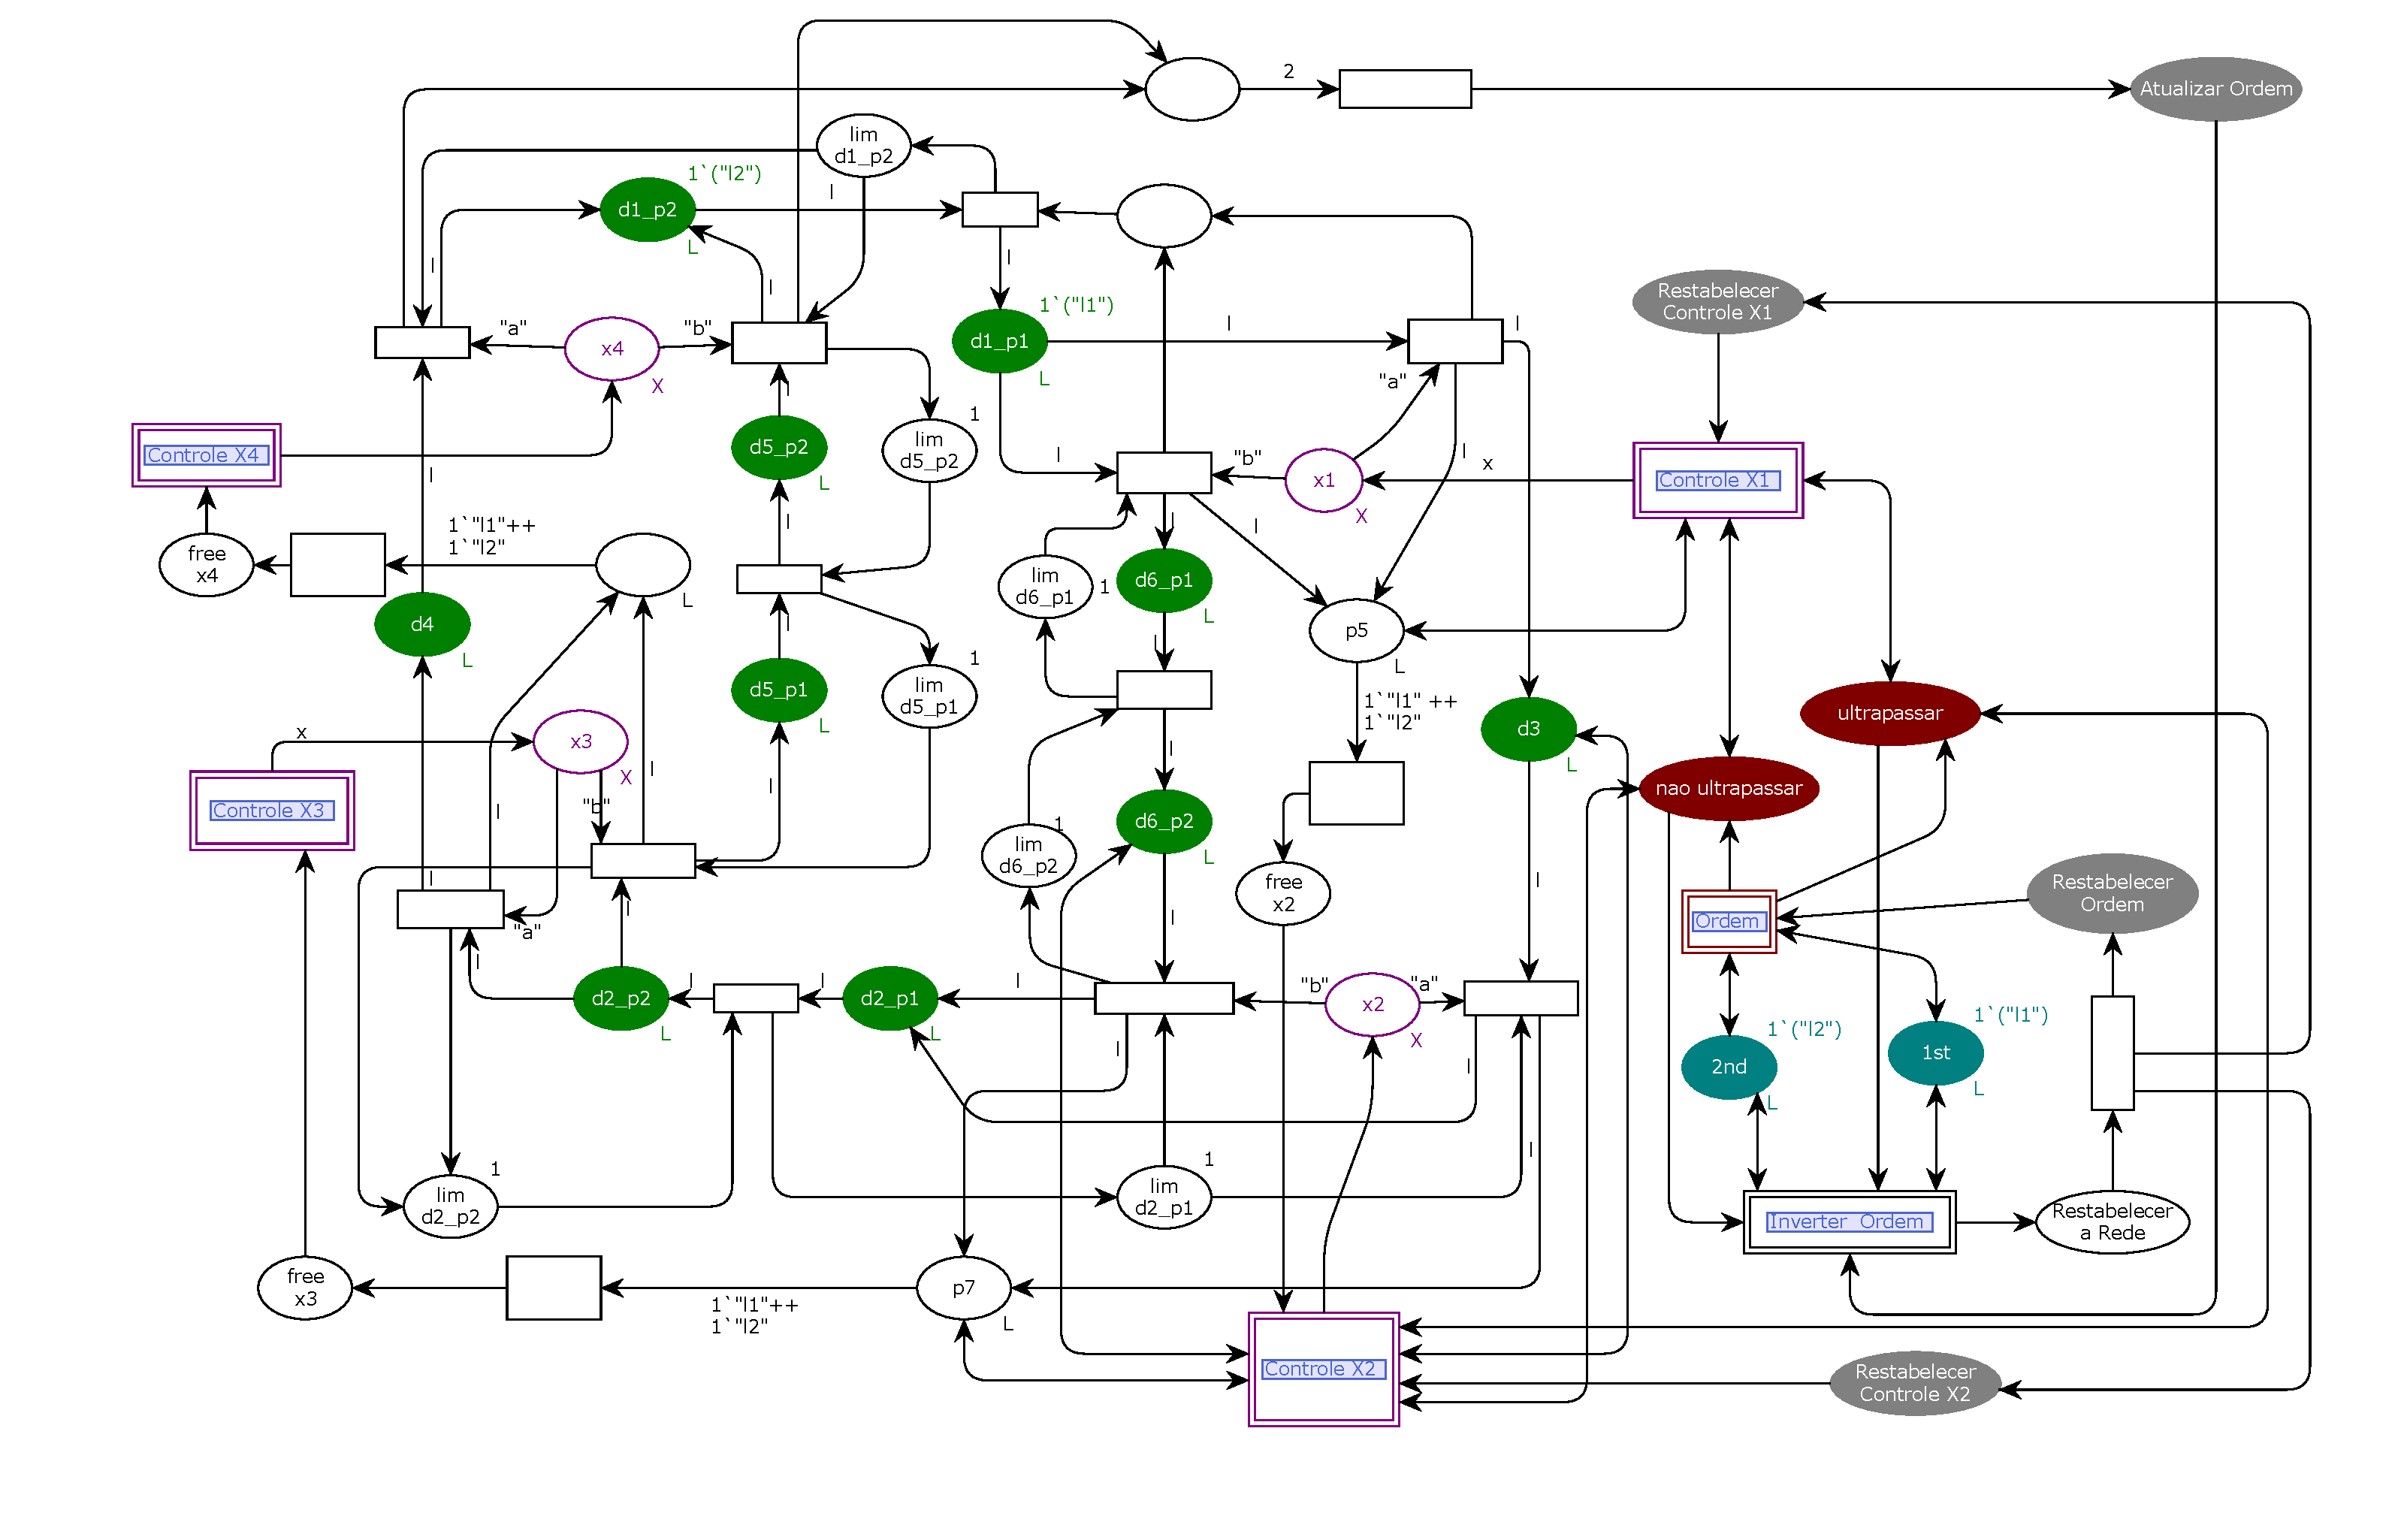
\includegraphics[width=1\linewidth]{figures/Simulation/Modelagem/rede_geral.eps}
    \legend{Fonte: Elaborado pelo autor.}
\end{figure}


\subsection{Modelagem da Pista}
\label{sub:model_pista}
A modelagem da pista foi feito através do conjunto de lugares e transições que representam o movimento e mecanismos pelos quais os vagões iram transitar, a modelagem completa dada pela figura \ref{fig:rede_geral} foi dividida em algumas máscaras (representação parcial da rede) para melhor visualização ao longo da sub seção. 

A figura \ref{fig:pista_RPC} demonstra os principais componentes das pista, tal que os lugares de $d_1$ a $d_6$ referem-se as curvas da pista representada na figura \ref{fig:pista_com_dois_agentes}. Observe que o conjunto de cores nesses lugares são o conjunto $L$, indicando que neles transitam as fichas do tipo vagões que podem ser "$l_1$" ou "$l_2$" como nos casos do lugar $d_1\_p_1$ e $d_1\_p_2$ respectivamente. Assim de modo análogo os arcos que referentes a movimentação das fichas do tipo \textit{L} são da variável tipo \textit{l} que controla os graus de saída e entrada das transições que movimentam os vagões ao longo da pista. Também é modelado os locais de junções e divisões, por exemplo no lugar $d_1\_p_1$ que representa a área $1$ da pista $d_1$ nela a pista sofre uma divisão, de modo que o vagão pode ir ou para a curva $d_6$ ou para a curva $d_3$ da pista. Os locais de junção ocorrem por exemplo na curva $d_2\_p_1$ da pista, em que recebe tanto os vagões que veem da pista $d_3$, quanto da pista $d_6$.
\begin{figure}[ht]
    \centering
    \caption{Máscara dos Componentes da pista na RPC}
    \label{fig:pista_RPC}
    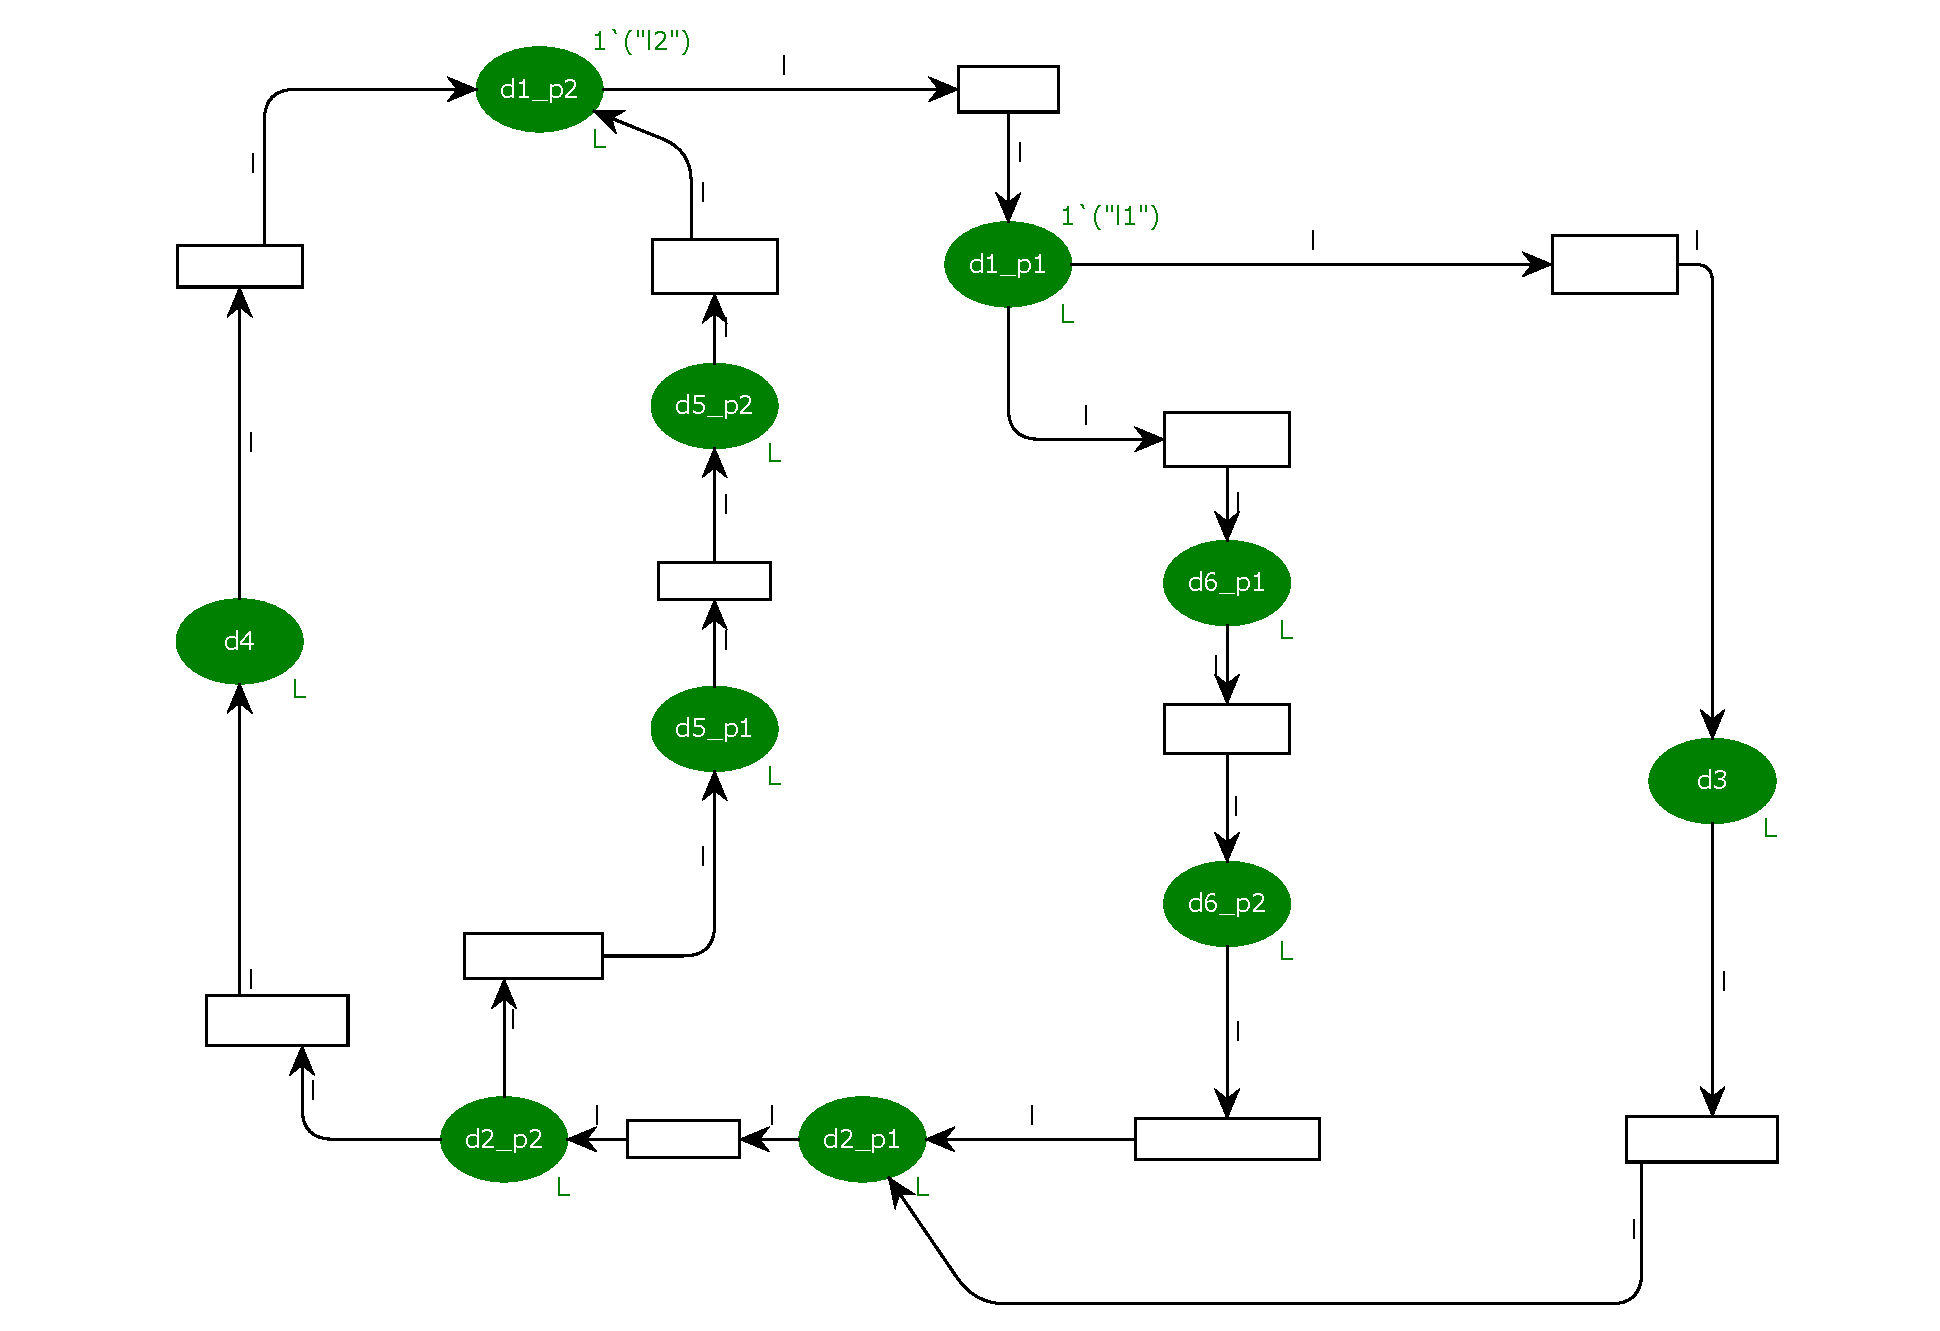
\includegraphics[width=1\linewidth]{figures//Simulation//Modelagem/pista.eps}
    \legend{Fonte: Elaborado pelo autor.}
\end{figure}

Para a modelagem da pista também é importante a implementação do conceito limitadores de região, que são lugares que controlam a quantidade de vagões por região, que para níveis de modelagem na RPC são importantes para evitar que dois vagões estejam na mesma região ao mesmo tempo. Os limitadores de região são implementados em algumas regiões como demonstrado na figura \ref{fig:limitadores_pista}, de modo que quando o vagão entra em determinada região é retirado uma ficha do lugar \textit{lim} ${d_x\_p_y}$, desabilitando a transição que permite a entrada de um vagão naquela região, tal ficha é devolvida quando o vagão que está sai para outra região. 

Por exemplo, note que para que uma ficha entre no lugar $d_5\_p_2$ é necessário que haja uma ficha no lugar \textit{lim} $d_5\_p_2$, e que ao entrar nessa região uma ficha é consumida e ao sair a ficha é retornada ao limitador garantido que somente um vagão ocupara aquela região por vez.

\begin{figure}[ht]
    \centering
    \caption{Máscara dos Componentes da pista com o controle das chaves na RPC}
    \label{fig:limitadores_pista}
    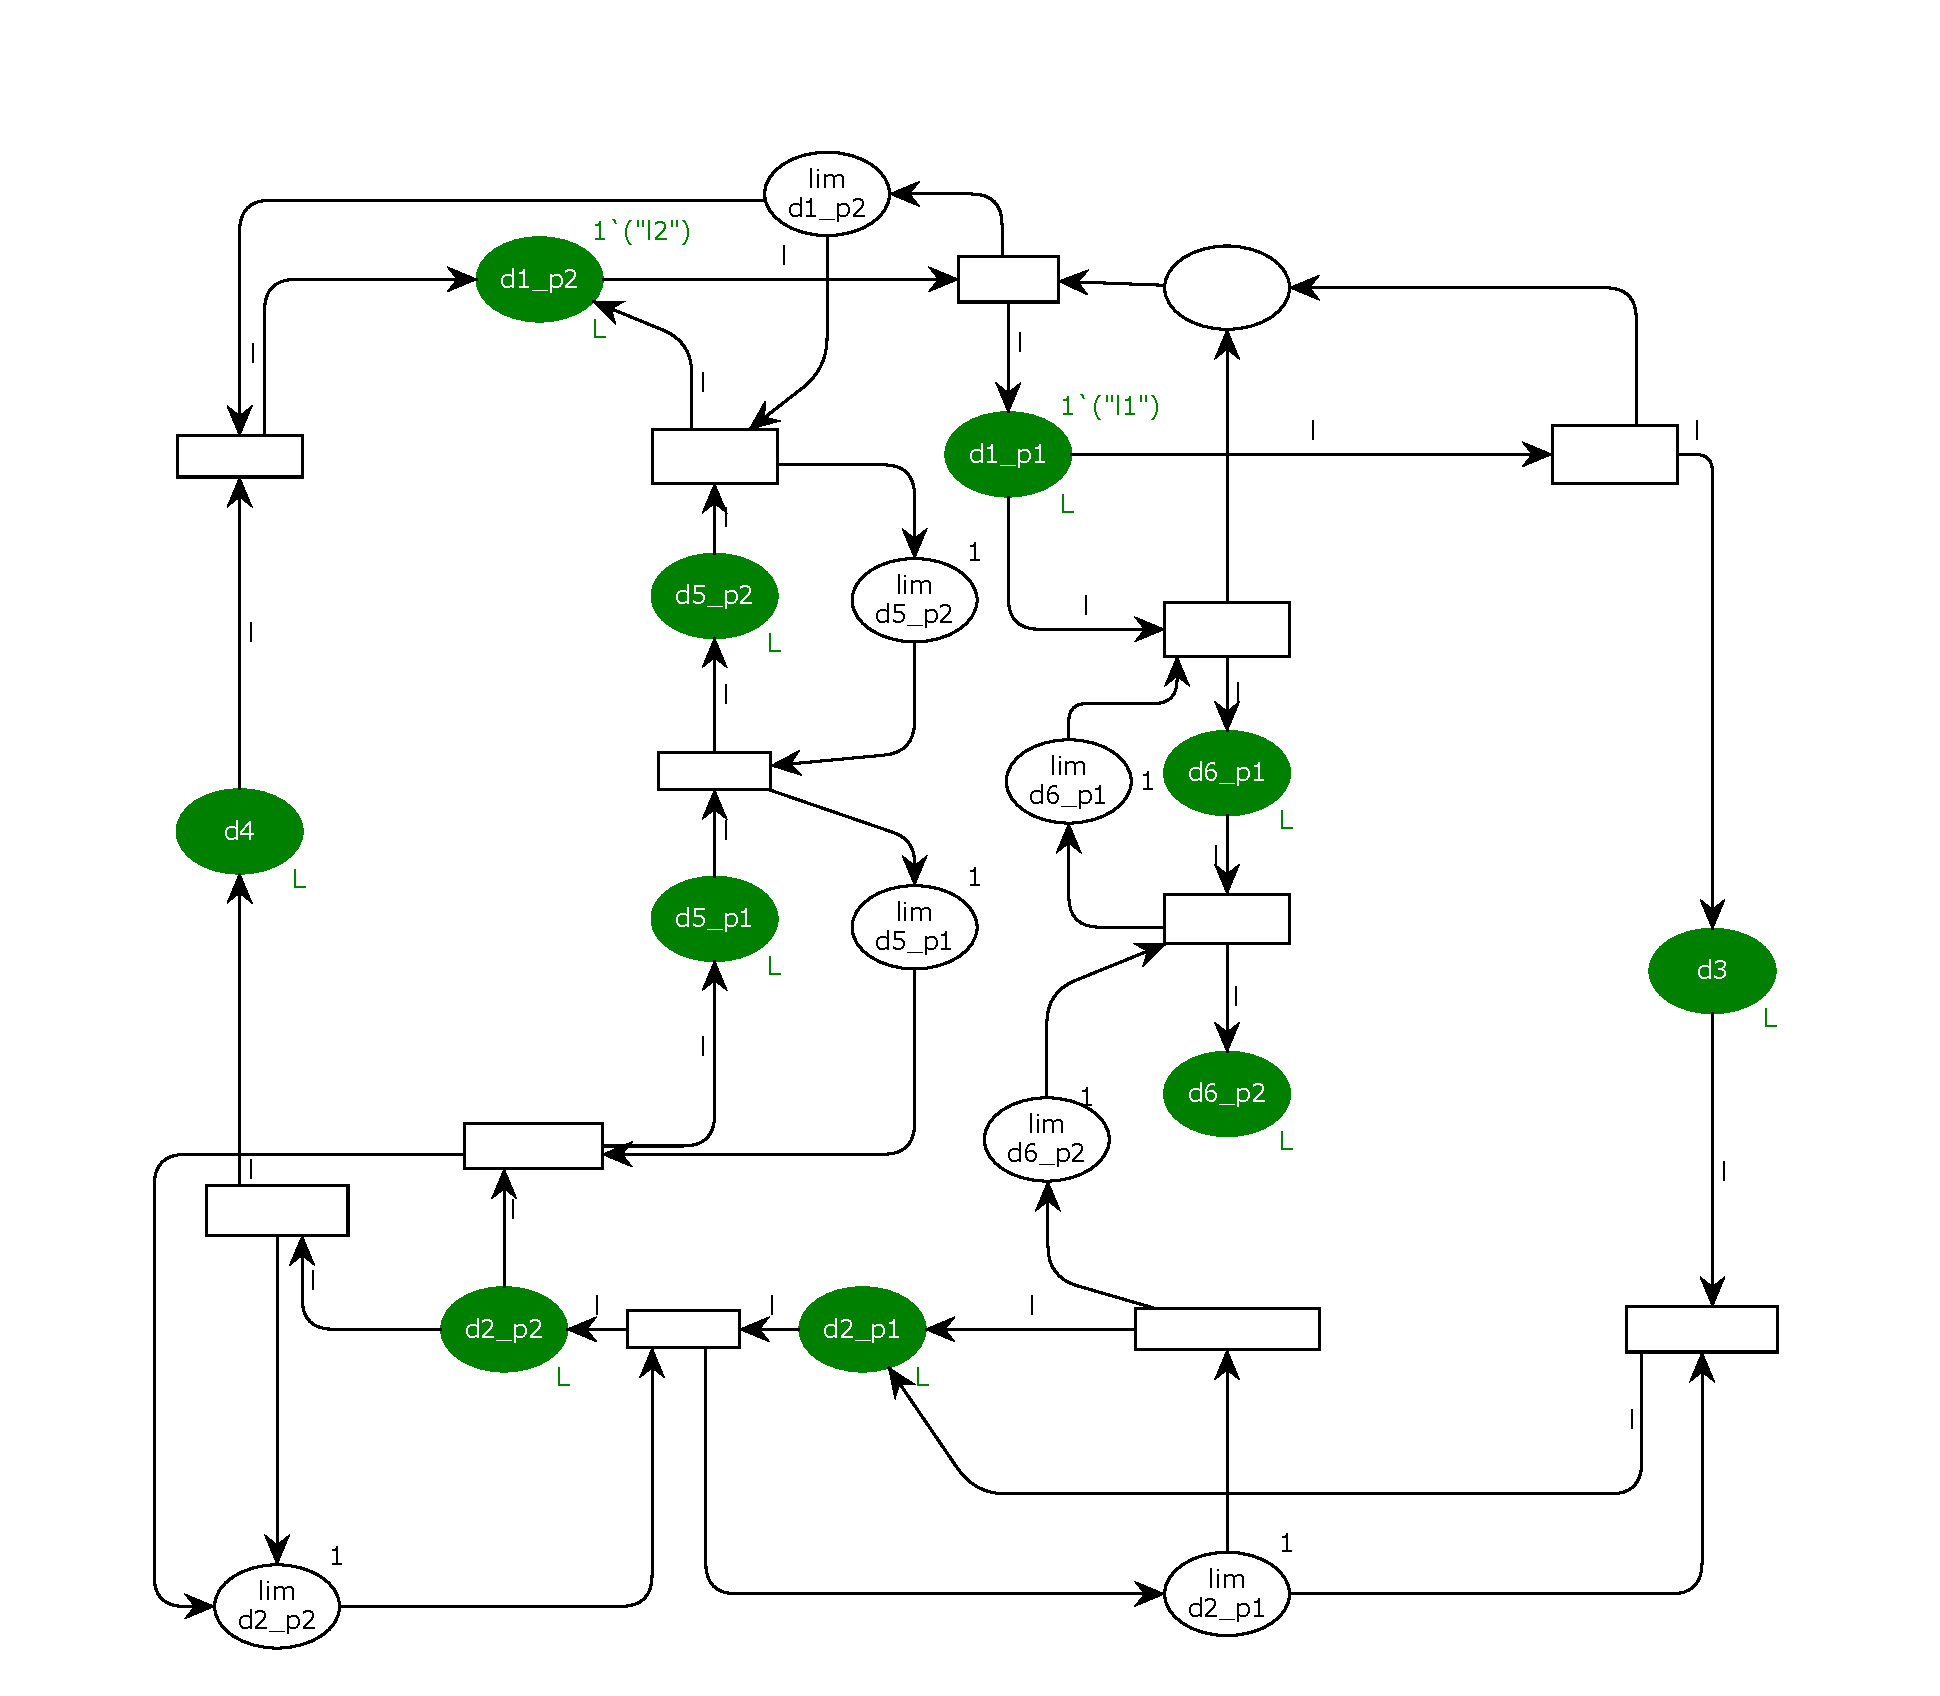
\includegraphics[width=1\linewidth]{figures//Simulation//Modelagem/limitadores_pista.eps}
    \legend{Fonte: Elaborado pelo autor.}
\end{figure}

Outro conceito fundamental na modelagem de uma RPC é o de reestabelecimento da rede, garantido que ao chegar no final do ciclo de uma volta a rede continue em funcionamento para um número ilimitado de iterações, tal reestabelecimento é demonstrado na figura \ref{fig:restabelecer_geral}. Note que após a segunda ativação da chave $X_4$ é dado o comando de atualizar a ordem vigente dos vagões e logo em seguida é dado o comando de \textit{Reestabelecer a Rede}, enviando a ficha para reestabelecer os \textit{Controles} $X_1 e X_2$ assim como o \textit{Controle de Ordem}.

\begin{figure}[ht]
    \centering
    \caption{Máscara dos Componentes de reestabelecimento na RPC}
    \label{fig:restabelecer_geral}
    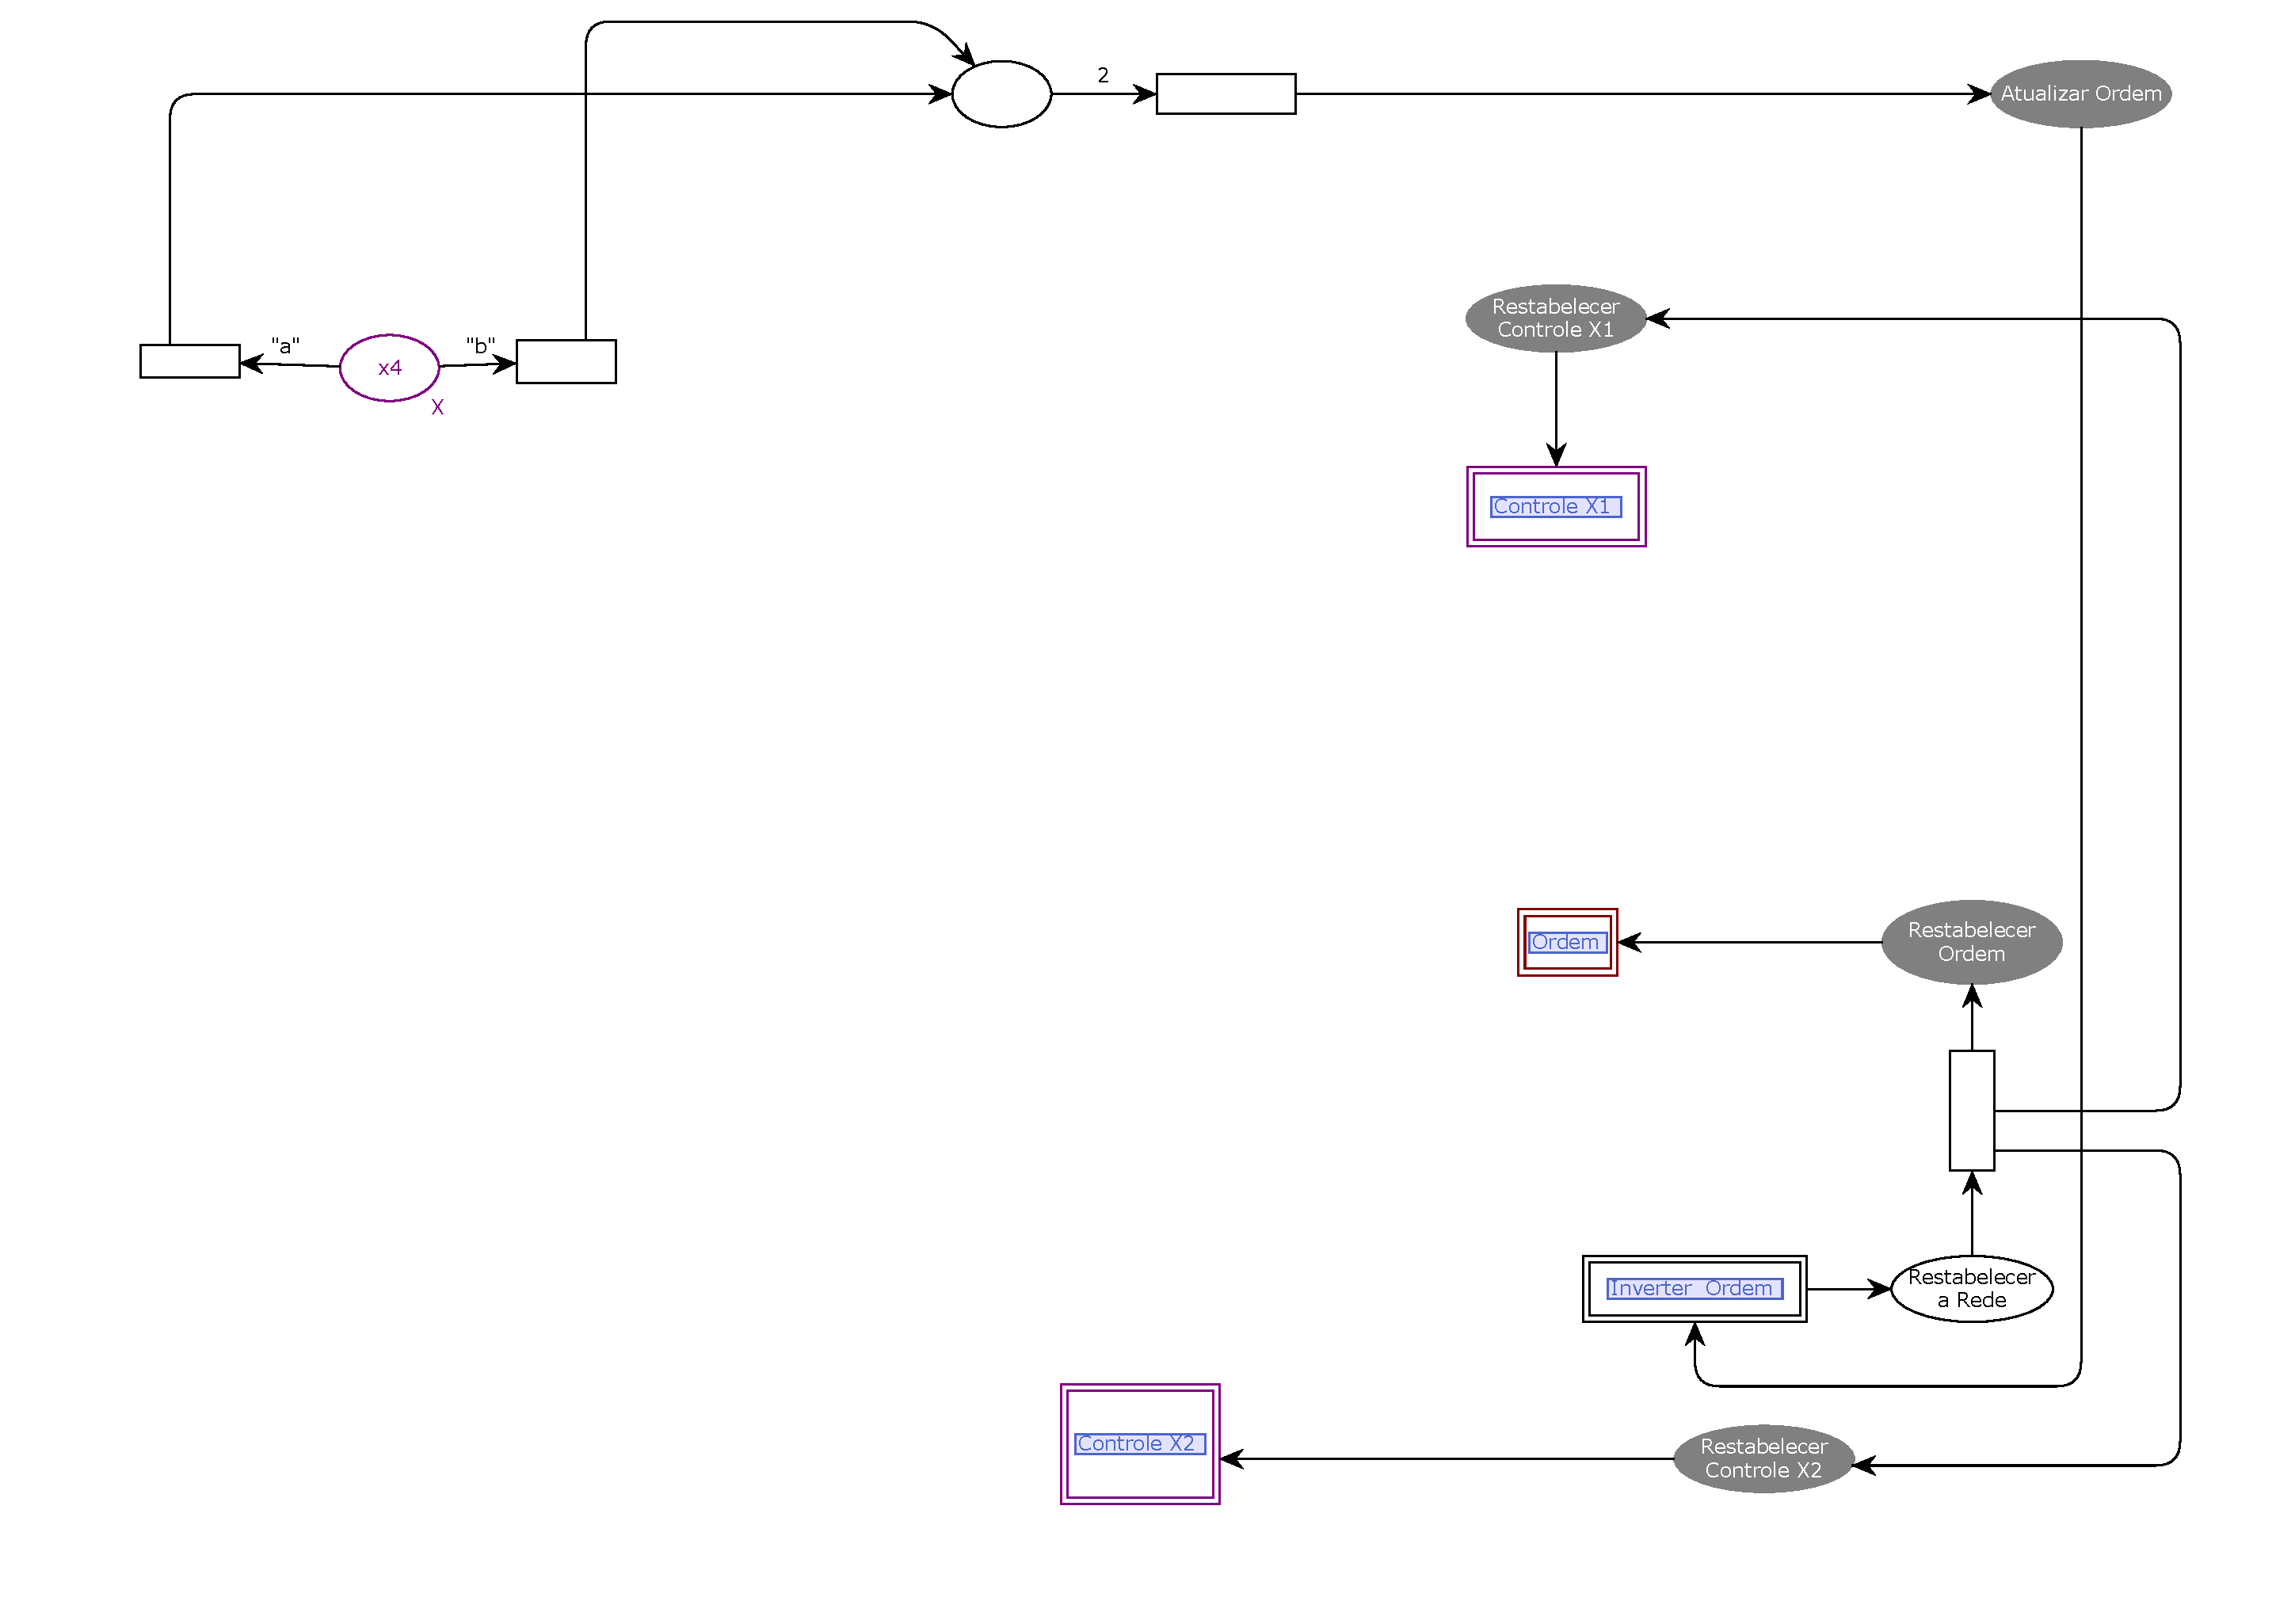
\includegraphics[width=1\linewidth]{figures/Simulation/Modelagem/restabelecer_geral.eps}
    \legend{Fonte: Elaborado pelo autor.}
\end{figure}

\clearpage
\subsection{Modelagem Controladores}
Considerando o modelo anterior na subseção \ref{sub:model_pista} de organização das pistas a figura \ref{fig:pista_chaves_RPC} representa além dos componentes fundamentas das curvas das pistas $d_1$ a $d_6$, os componentes de chaves \textit{X}, com as transições hierárquicas de \textit{Controle} $X_1$ a \textit{Controle} $X_4$. Observe que nos pontos de junção e divisão se encontroam os locais $X_1$ a $X_4$, que pertencem ao conjunto \textit{X} que podem receber fichas do tipo "a" ou "b" como explicado no quadro \ref{qua:variaveis_RPC}, tais lugares controlam as condições de acionamento das transições ligadas os arcos de saída. 

Por exemplo, dado um ficha "1`$(l_1)$" no lugar $d_1\_p_1$ quem vai definir qual transição será habilita, se para ir para a pista $d_3$ ou para a pista $d_6$, será a ficha no lugar $x_1$, que é controlada pela transição hierárquica \textit{Controle} $X_1$. Tal que dependendo da ficha que o local \textit{X} receber pelos respectivos Controladores será habilitada e desabilitada as transições que ligam as curvas ao longo da pista. 
\begin{figure}[ht]
    \centering
    \caption{Máscara dos Componentes da pista com o controle das chaves na RPC}
    \label{fig:pista_chaves_RPC}
    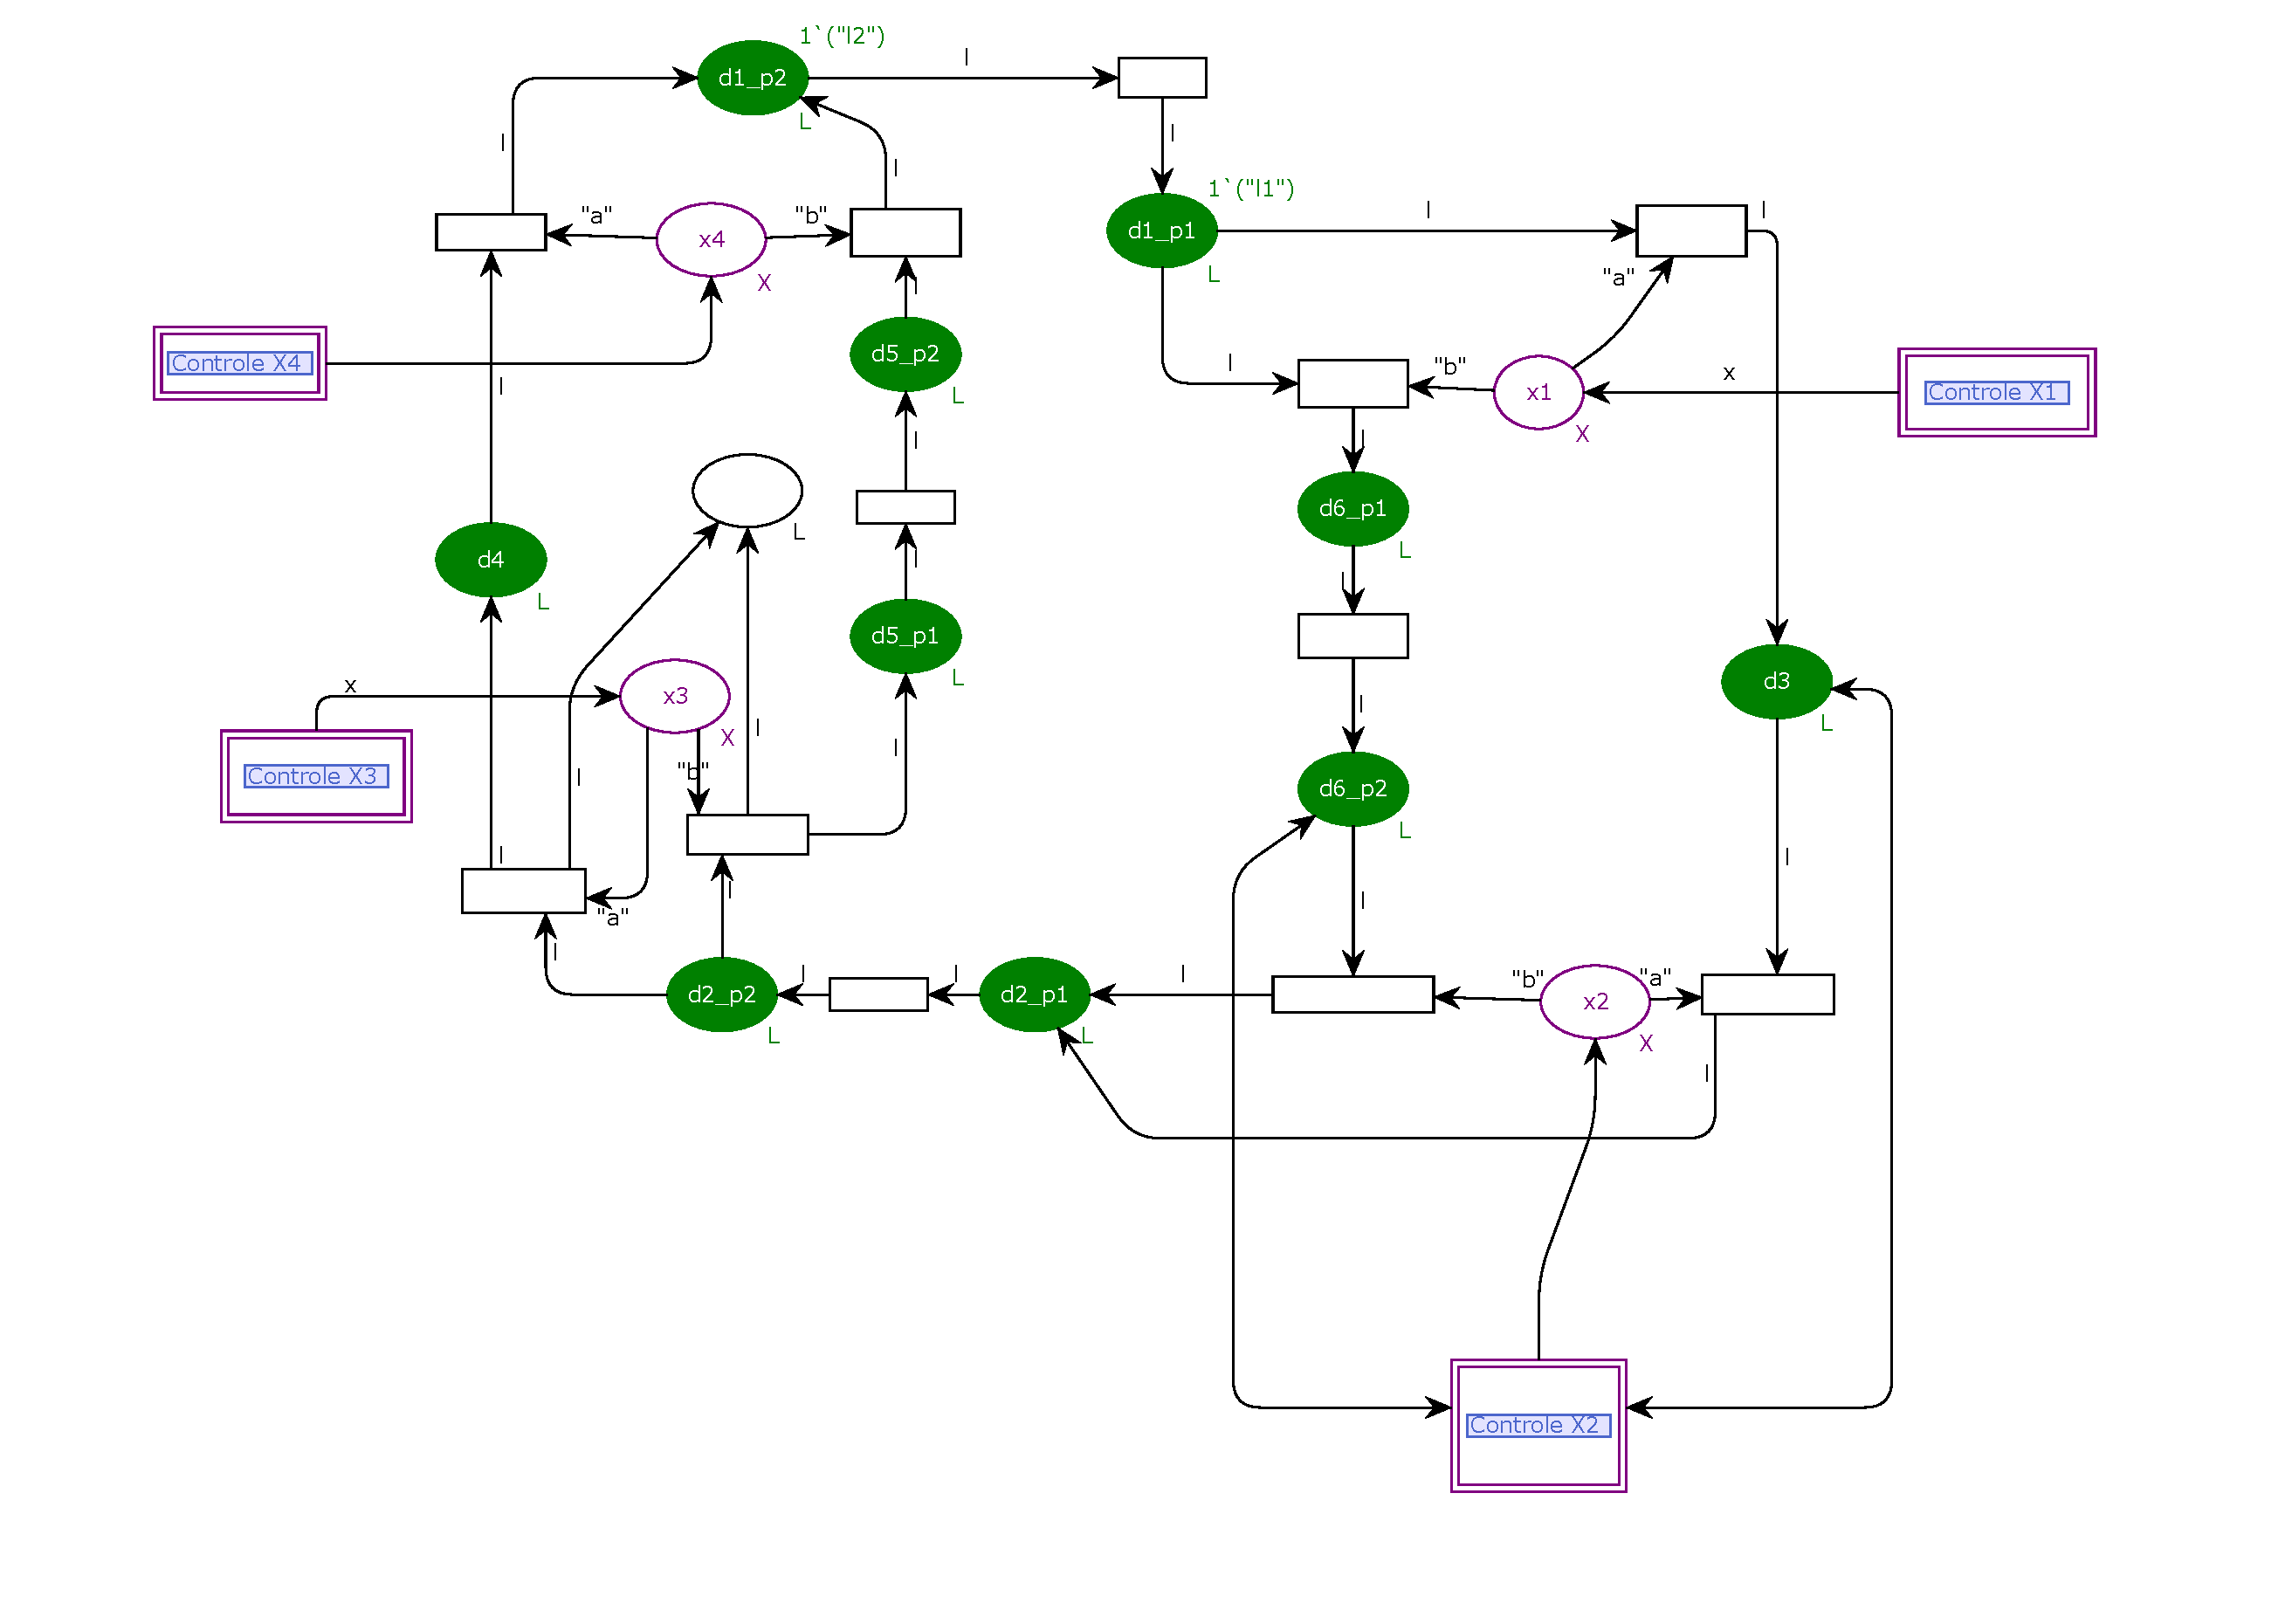
\includegraphics[width=1\linewidth]{figures//Simulation//Modelagem/pista_com_chaves.eps}
    \legend{Fonte: Elaborado pelo autor.}
\end{figure}

Na modelagem dos controladores, é essencial assegurar a comunicação entre os elementos da pista em certos momentos, permitindo que os controladores tomem decisões com base nas posições dos vagões. Um exemplo dessa comunicação é ilustrado na Figura \ref{fig:free_control}. Em algumas transições conectadas às chaves, a informação sobre qual vagão passou pela região é transmitida à medida que as transições são acionadas. Posteriormente, essas informações são fornecidas, direta ou indiretamente, aos controladores.

Por exemplo, note que nas transições ligadas ao lugar $X_2$ possuem lugar de saída definida no conjunto L, de modo que ao passar algum vagão naquela região, a informação de qual vagão passou é processada pelo \textit{Controle} $X_2$. Posteriormente ao se passar os dois vagões diferentes a transição ligada ao lugar \textit{free} $x_3$ é habilitada, transmitindo a informação de que já se passaram aqueles dois tipos de vagões naquela região, para a tomada de decisão do \textit{Controle} $X_3$.

\begin{figure}[ht]
    \centering
    \caption{Máscara dos Componentes de controle das chaves e comunicadores na RPC}
    \label{fig:free_control}
    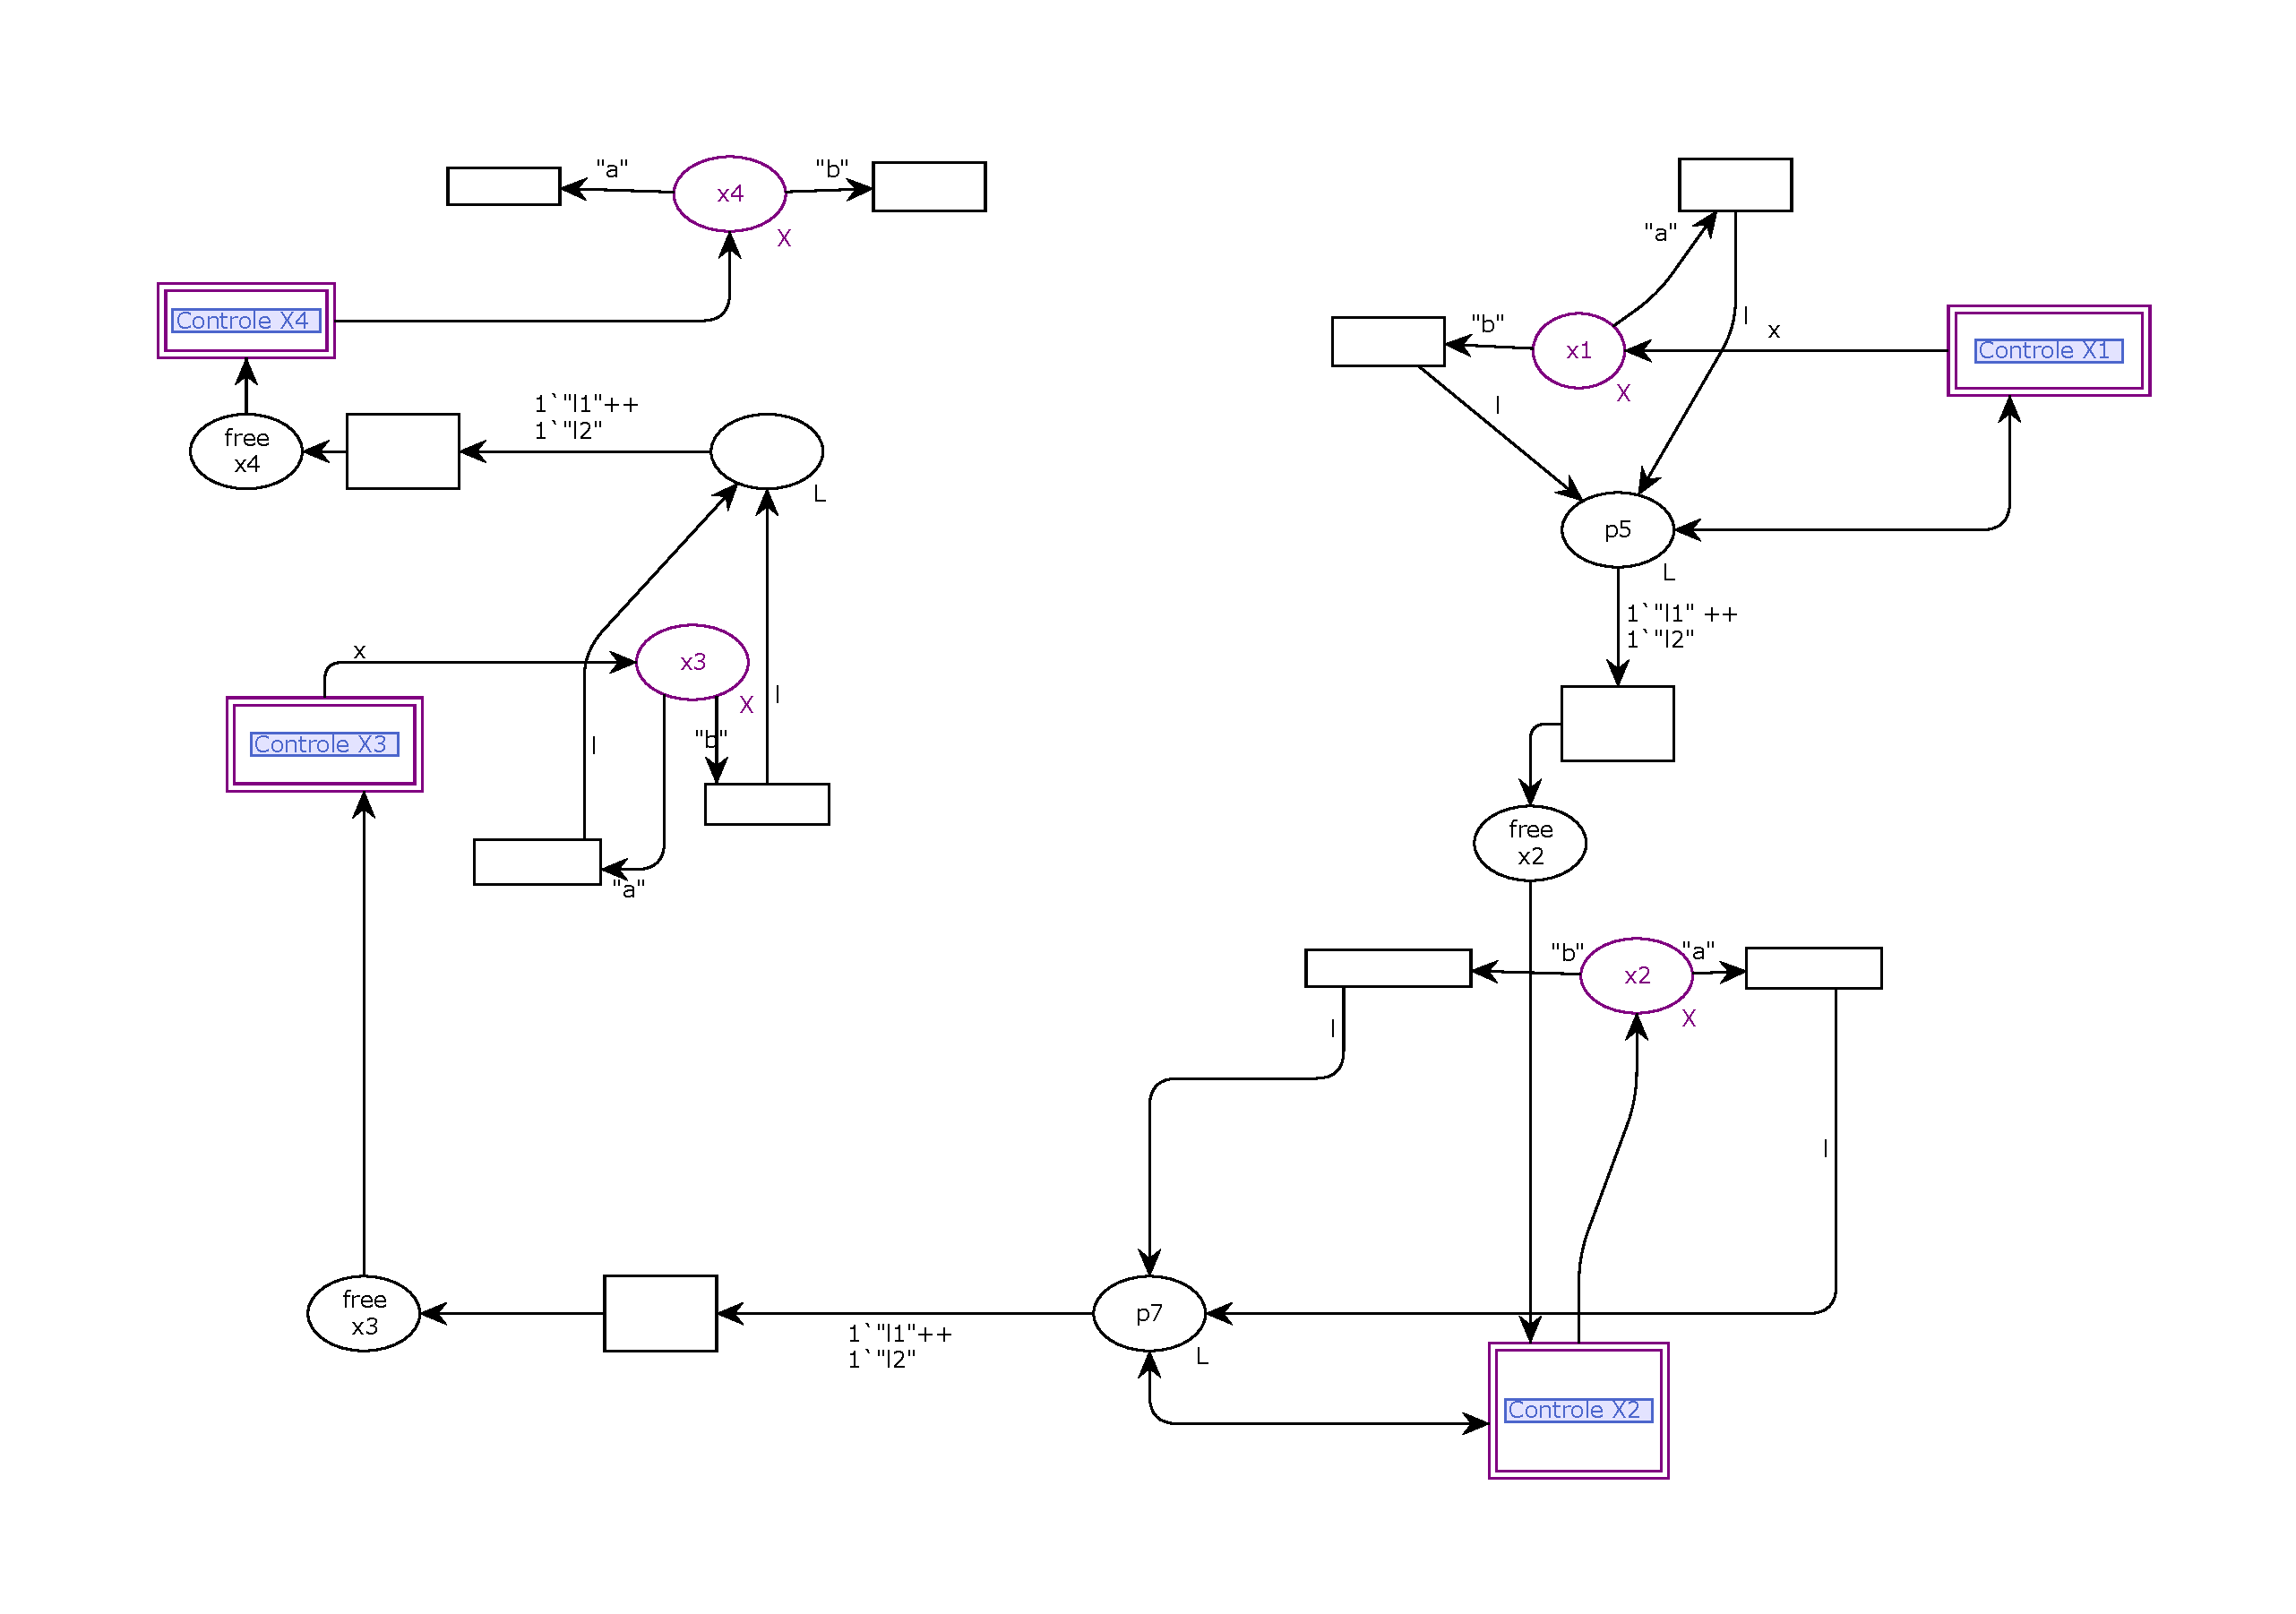
\includegraphics[width=1\linewidth]{figures//Simulation//Modelagem/free_control.eps}
    \legend{Fonte: Elaborado pelo autor.}
\end{figure}


Em um nível hierárquico abaixo do nível da pista, como demonstrado na figura \ref{fig:hierarquia_RPC} estão os \textit{Controladores} $x_1$ a $x_4$, que serão detalhados a seguir. 

O \textit{Controlador} $X_1$ referente a transição \textit{Controle} $X_1$ com borda vermelha na figura \ref{fig:free_control}, é demonstrado na figura \ref{fig:controle_x1}. Note que a rede de Controle de $X_1$, possui alguns lugares com subscrição denominadas de \textit{IN}, \textit{OUT} ou \textit{IN/OUT}, que são diretamente relacionadas aos lugares externos a rede, estabelecendo uma comunicação com lugares pertencentes ao nível hierárquico superior. Alguns lugares como $x1$ e $p5$ já foram demonstrados na máscara de componentes na figura \ref{fig:free_control}, outros serão demonstrados na subseção \ref{sub:model_ord} referente a modelagem de ordenação dos vagões.

Para o controle do lugar $X_1$ note que a rede possui inicialmente uma ficha no lugar $p_1$, de modo que dependendo do comando de ultrapassar ou não ultrapassar a transição $t_2$ ou $t_1$ será acionada, respectivamente. O acionamento primeiro coloca ficha de posição "a" ou "b" na chave $X_1$ e posteriormente a posição "b" pela transição $t_3$ pós a passagem do primeiro vagão sinalizada pelo lugar $p_5$. Após os dois comandos de posição serem utilizados a rede aguarda o comando externo de restabelece o controle para assim, reiniciar a rede para o estado inicial e começar um novo ciclo.

\begin{figure}[ht]
    \centering
    \caption{Rede referente ao controle hierárquico X1 na RPC}
    \label{fig:controle_x1}
    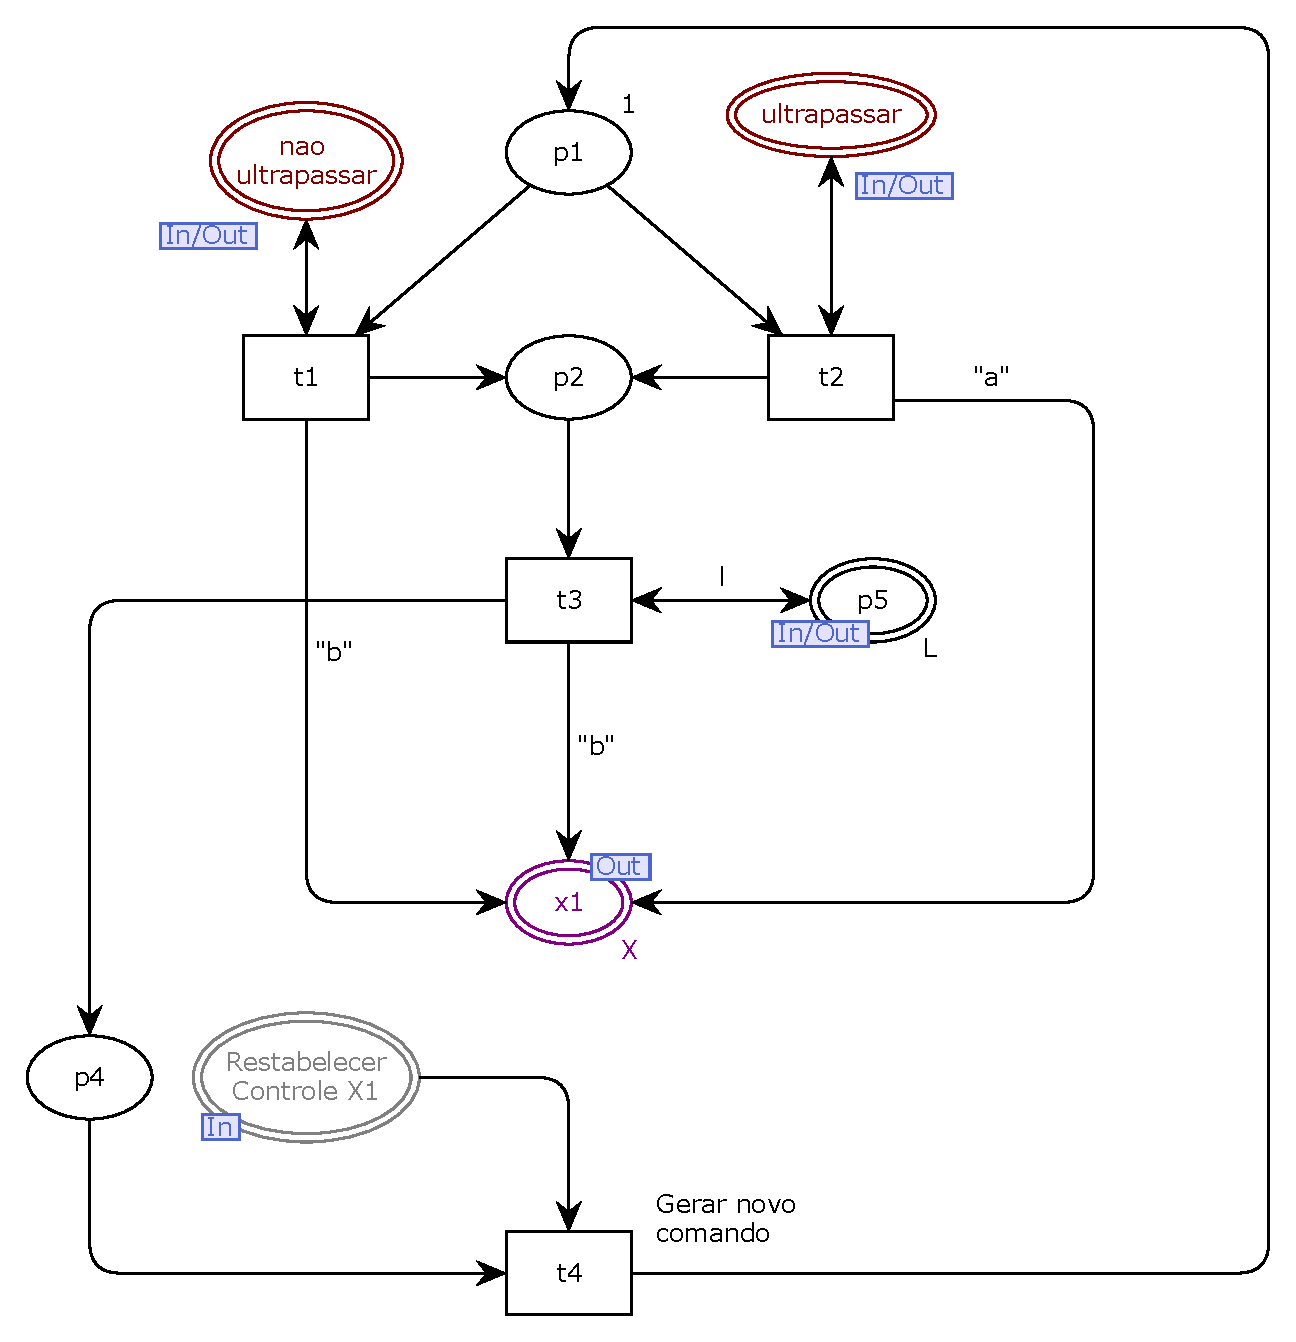
\includegraphics[width=0.5\linewidth]{figures//Simulation//Modelagem/controle_x1.eps}
    \legend{Fonte: Elaborado pelo autor.}
\end{figure}

A RPC referente a transição \textit{Controle} $X_2$ é demonstrado na figura \ref{fig:controle_x2}. Tal controle tem como objetivo primeiramente receber o vagão da pista $d_6$, ou seja do menor caminho e posteriormente, analisar caso tenha tido o comando de ultrapassagem o próximo vagão é esperado na pista $d_3$, caso contrário virá novamente pela pista $d_6$. Para alcançar tal objetivo primeiramente a estrutura da rede recebe uma ficha vinda da pista de \textit{free} $x_2$ ativando a transição $t_9$ que espera o vagão chegar em $d_6$, ao ser identificado na curva é liberada primeiramente a ficha para X2 "b". Posteriormente, dependendo do comando relacionado à ultrapassagem é acionado $t_13$ ou $t_12$, com as fichas respectivamente em $p_11$ ou $p_10$, é esperado que chegar uma ficha no lugar $p_7$ indicando que já pode dar o segundo comando para a chave, por fim é dado o comando de posição "a" ou "b" para a chave caso $t_8$ seja acionado ou $t_7$, respectivamente. Ao fim do ciclo a rede espera uma ficha para restabelecer o \textit{Controle} $X_2$.

\begin{figure}[ht]
    \centering
    \caption{Rede referente ao controle hierárquico X2 na RPC}
    \label{fig:controle_x2}
    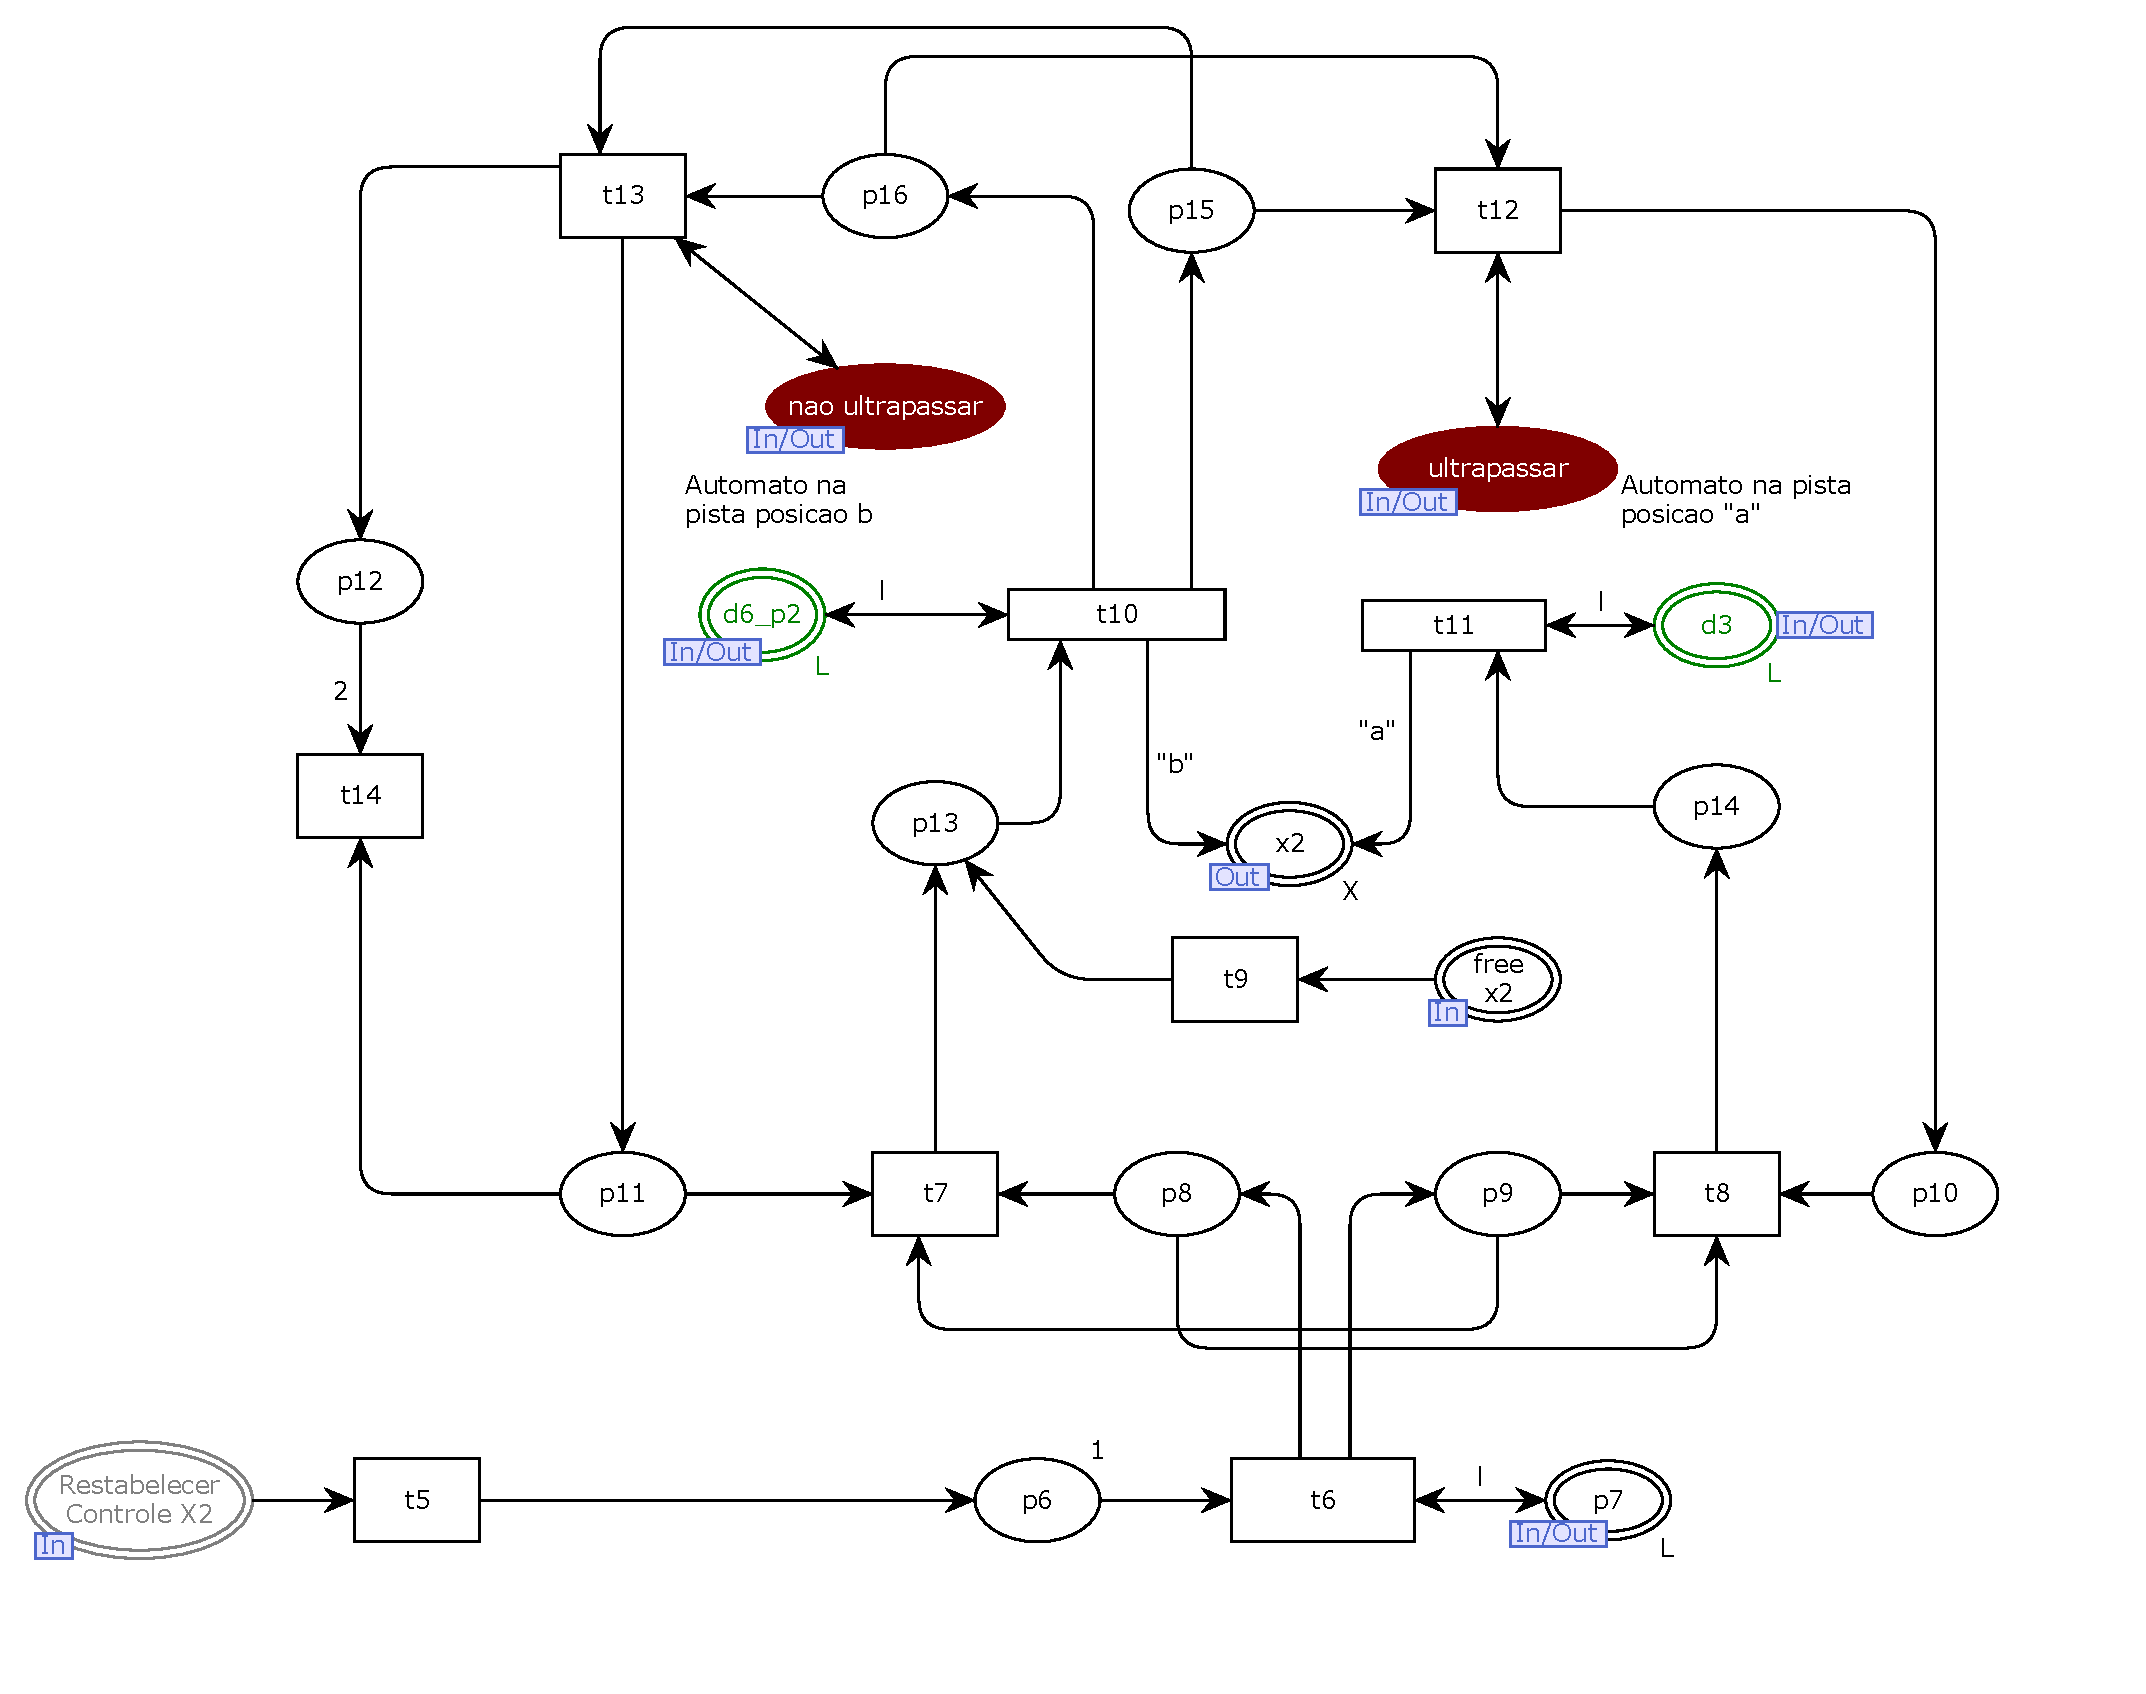
\includegraphics[width=0.9\linewidth]{figures//Simulation//Modelagem/controle_x2.eps}
    \legend{Fonte: Elaborado pelo autor.}
\end{figure}

A RPC referente ao controlador $X_3$ e $X_4$, possuem estruturas e comportamentos idênticos como demonstrados na figura \ref{fig:controle_x3} e \ref{fig:controle_x4}. Como no escopo da simulação o local de ultrapassagem foi fixado no \textit{Controle} $X_1$, o objetivo do \textit{Controle} $X_3$ e \textit{Controle} $X_4$ é apenas garantir que uma vez liberado o controle para o controlador através do lugar \textit{free} $x_3$ ou $x_4$ seja colocada a ficha de posição \textit{"b"}, ou seja o menor caminho para o vagão que vinher.

\begin{figure}[ht]
    \centering
    \caption{Rede referente ao controle hierárquico X3 na RPC}
    \label{fig:controle_x3}
    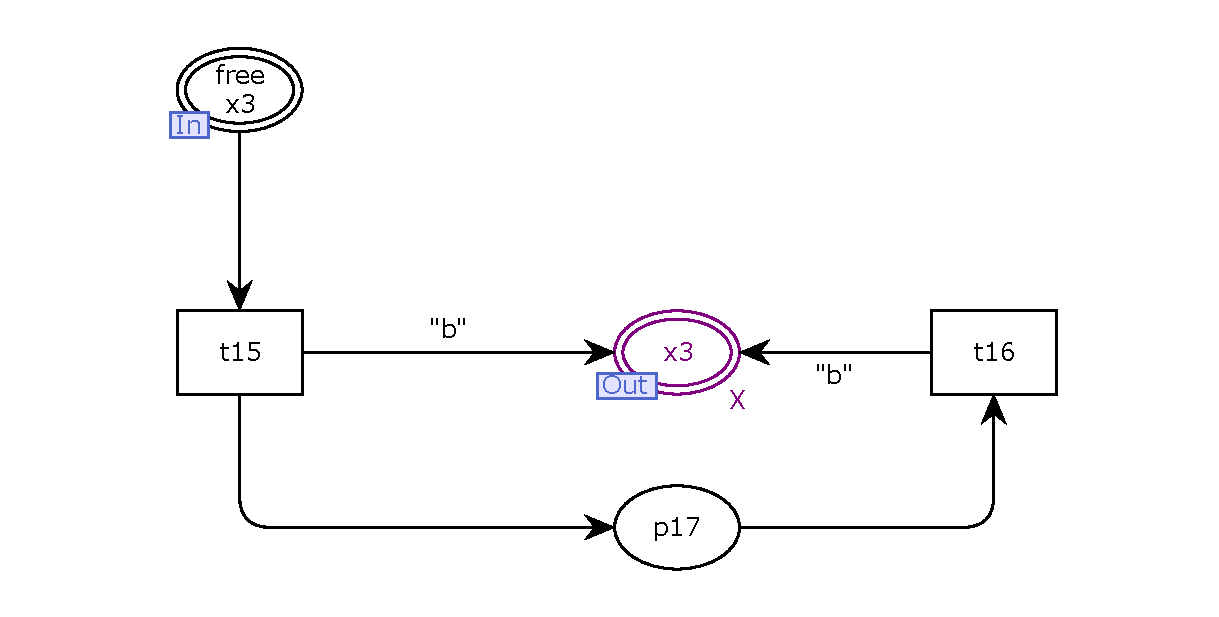
\includegraphics[width=0.6\linewidth]{figures//Simulation//Modelagem/controle_x3.eps}
    \legend{Fonte: Elaborado pelo autor.}
\end{figure}

\begin{figure}[ht]
    \centering
    \caption{Rede referente ao controle hierárquico X4 na RPC}
    \label{fig:controle_x4}
    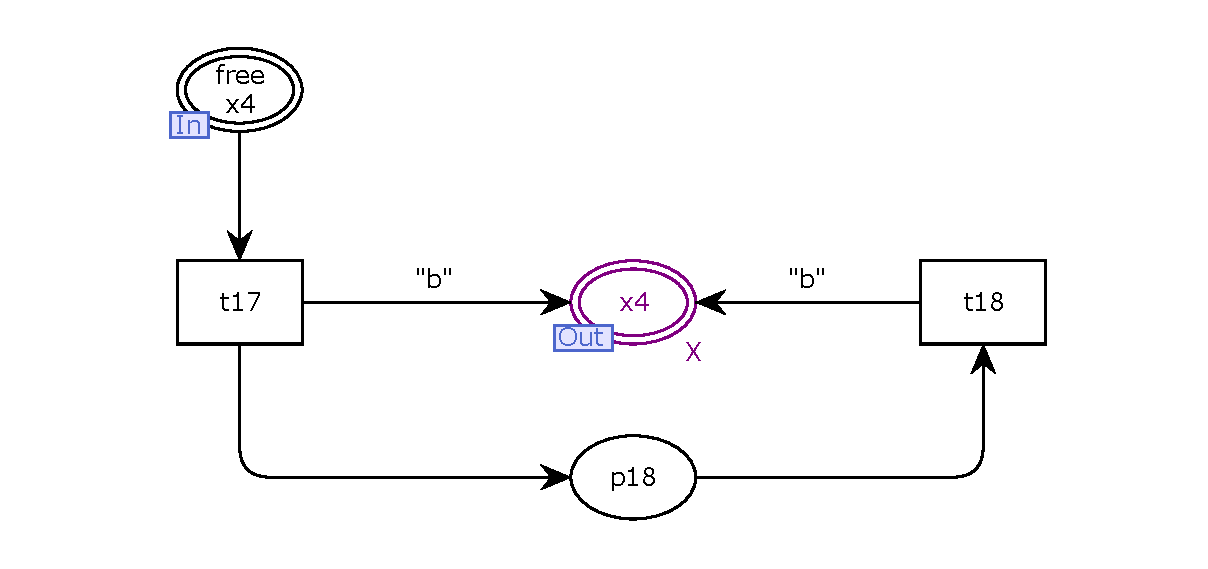
\includegraphics[width=0.6\linewidth]{figures//Simulation//Modelagem/controle_x4.eps}
    \legend{Fonte: Elaborado pelo autor.}
\end{figure}

\clearpage 
\subsection{Modelagem Ordenação dos vagões}
\label{sub:model_ord}
Na hierarquia trabalhada referente a figura \ref{fig:hierarquia_RPC}, que do modelo hierárquico referente a RPC, será demonstrado agora as redes relacionadas aos comando de coordenação dos vagões. Na camada de cima da hierarquia da pista as transições e lugares de ordem e inversão de ordem possuem comunicação principal com os controladores, como demonstrado na máscara do primeiro nível hierárquico na figura \ref{fig:pista_ordem}. Note que as informações de ultrapassagem e não ultrapassagem tem comunicação contro os \textit{Controladores} $X1$ e $X2$ e quem gerencia o primeiro($1_{st}$) e segundo($2_{nd}$) lugar são os dois componentes de \textit{Ordem} e\textit{ Inversão de Ordem}.

\begin{figure}[ht]
    \centering
    \caption{Máscara de componentes relacionados a ordem na RPC}
    \label{fig:pista_ordem}
    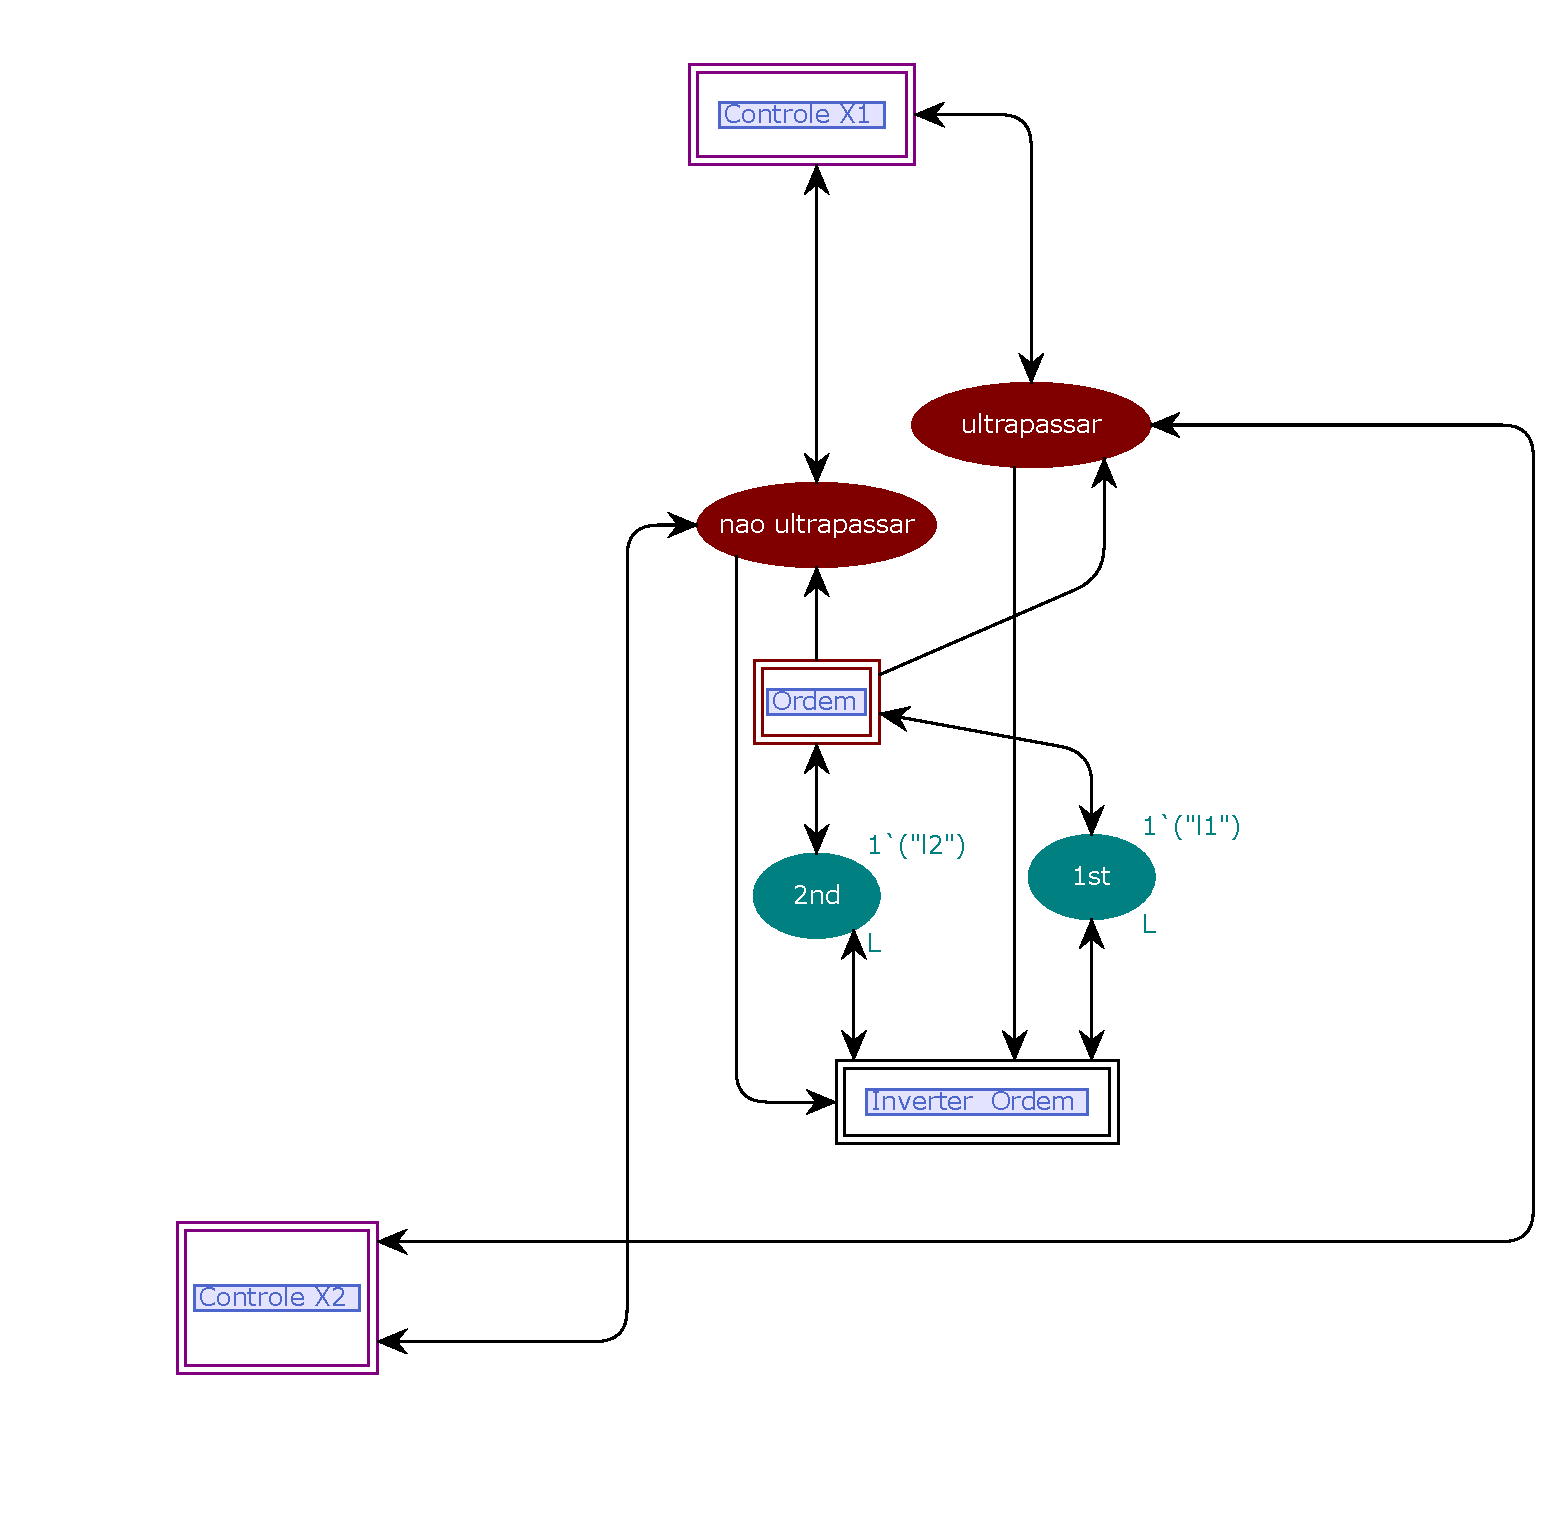
\includegraphics[width=0.8\linewidth]{figures//Simulation//Modelagem/pista_ordem.eps}
    \legend{Fonte: Elaborado pelo autor.}
\end{figure}

A transição hierárquica do componente de \textit{Ordem} é definida através da RPC demonstrada na figura \ref{fig:ordem}, para melhor compreensão a mesma foi dividade em duas máscaras uma de geração de comando e outra de restabelecimento da rede para geração de um novo comando.

\begin{figure}[ht]
    \centering
    \caption{Rede referente ao componente de Ordem na RPC}
    \label{fig:ordem}
    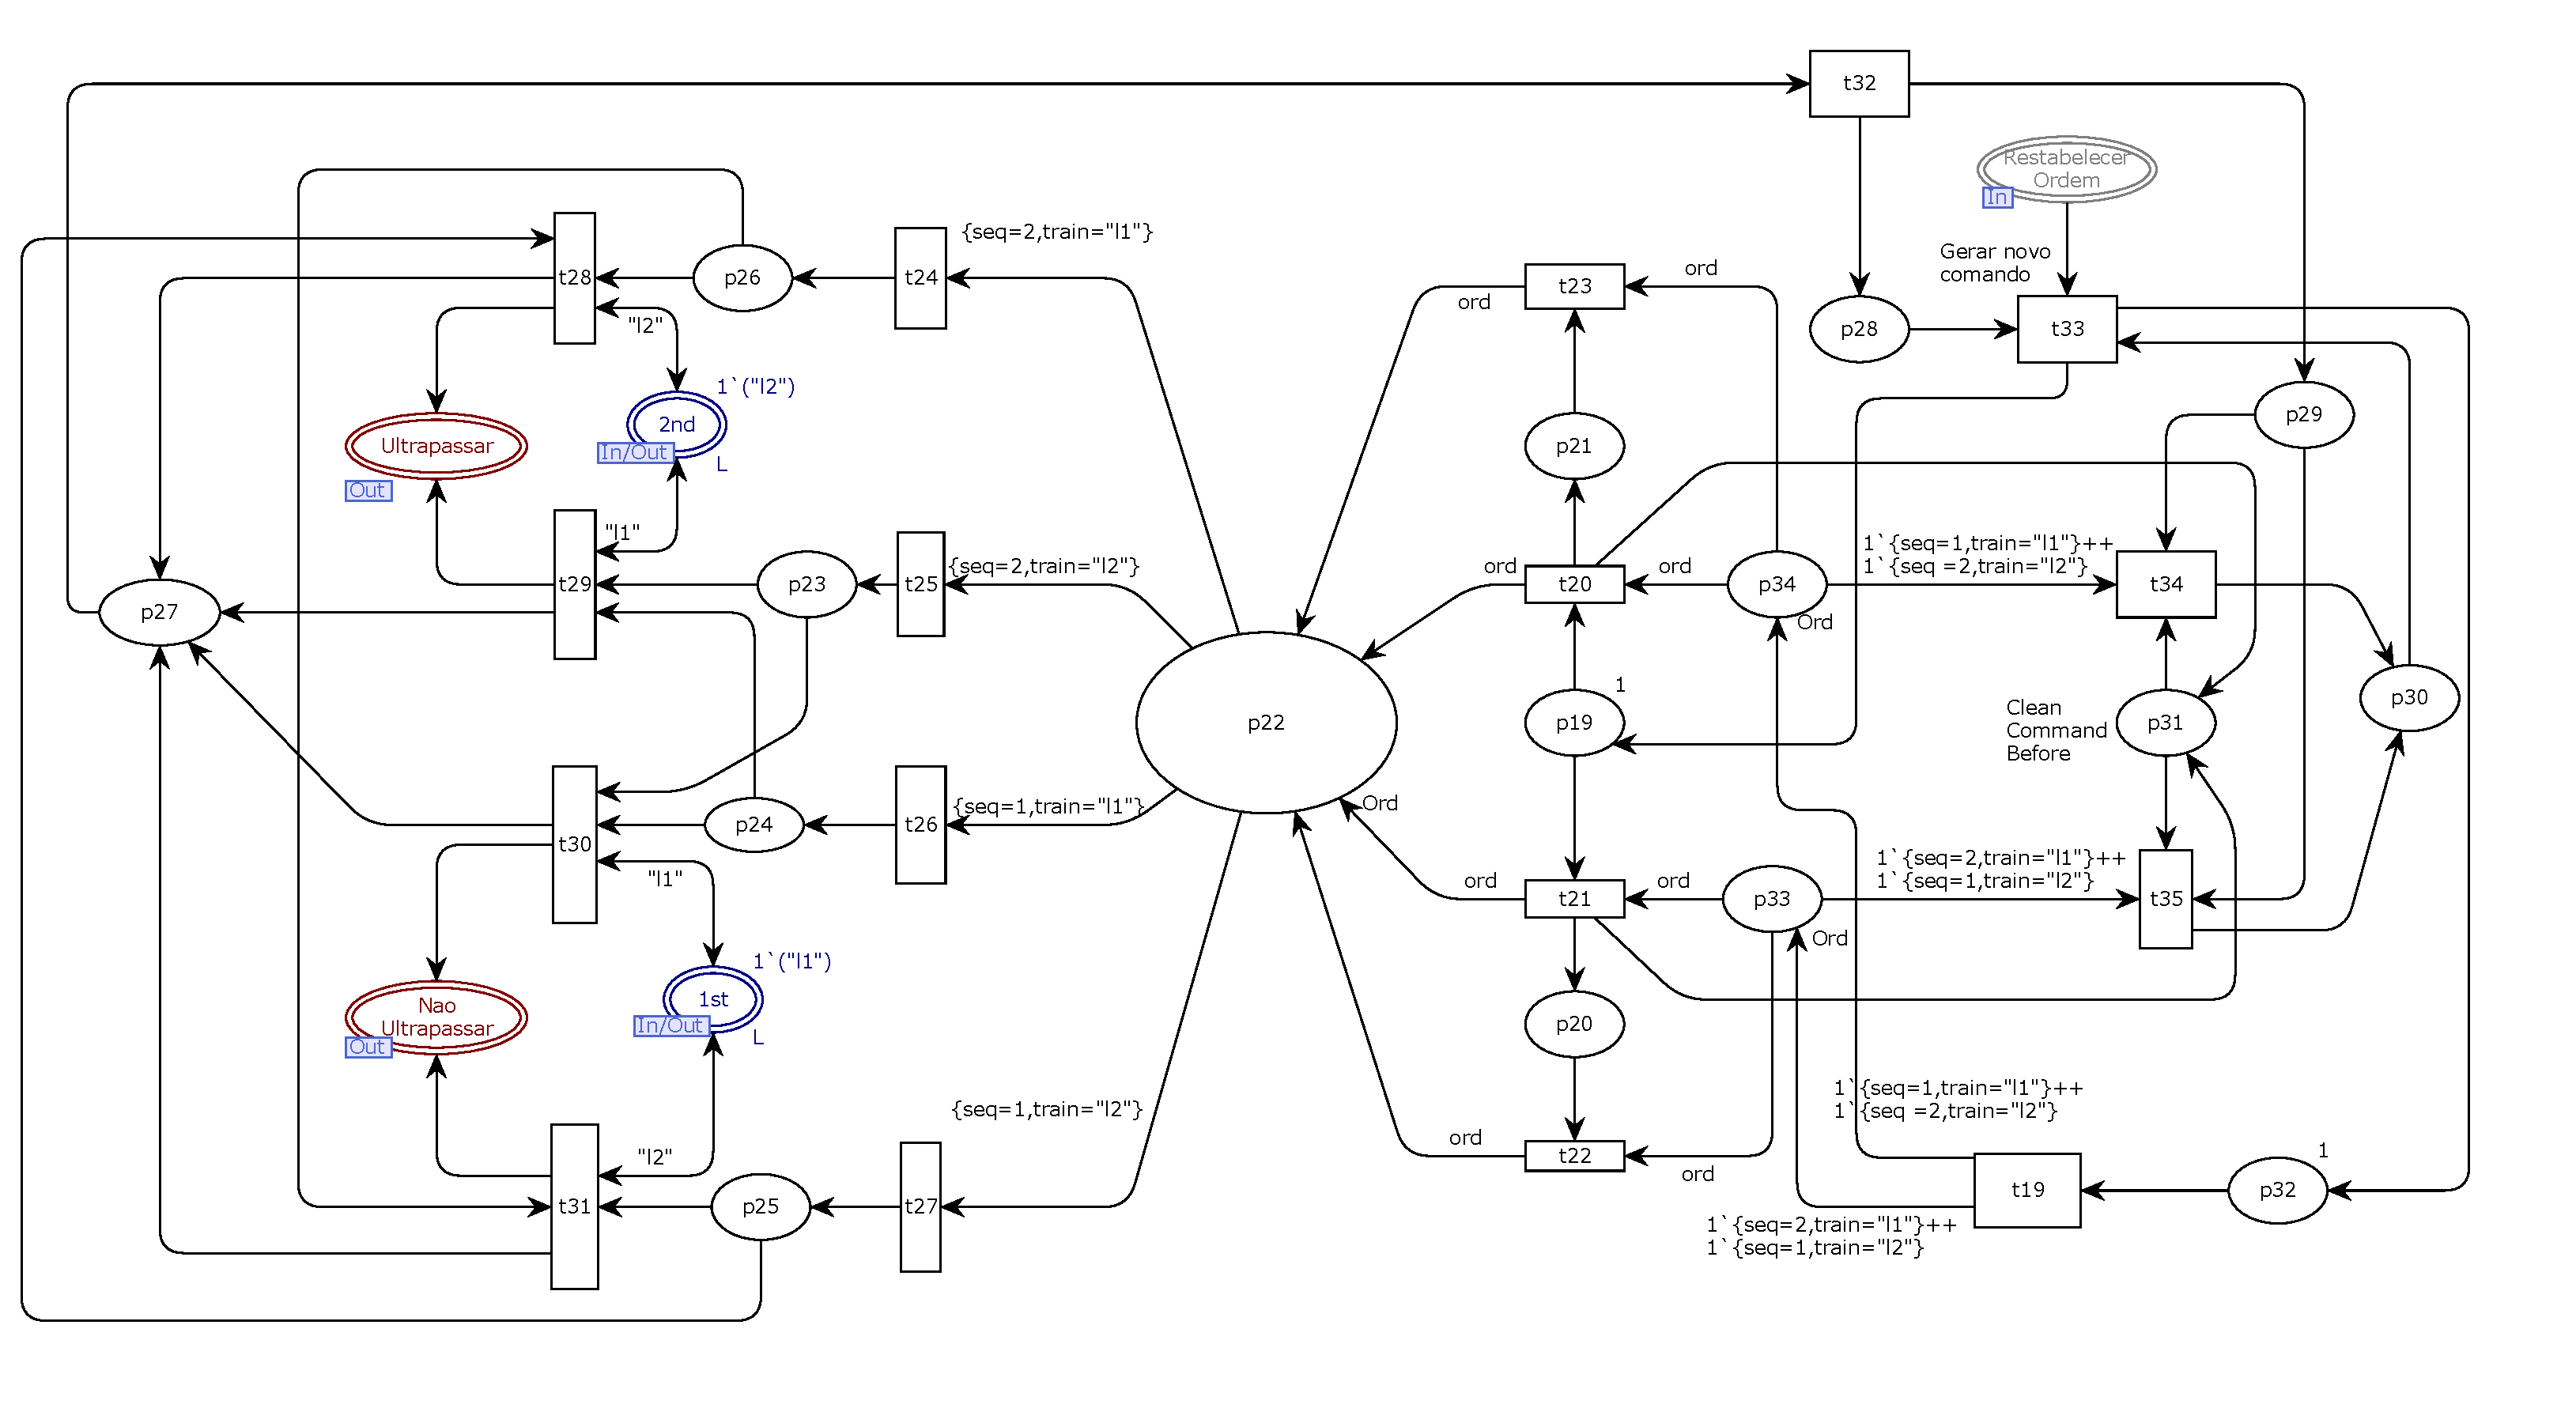
\includegraphics[width=1\linewidth]{figures//Simulation//Modelagem/ordem.eps}
    \legend{Fonte: Elaborado pelo autor.}
\end{figure}

Na geração do comando referente a ultrapassagem ou não ultrapassagem a parte da rede responsável é demonstrada na figura \ref{fig:geracao_ordem}, tal que no início da rede na transição $t_{19}$, são carregados dois comandos o primeiro comando que é recebido pelo lugar $p_{34}$ é o par da do vagão $l_1$ na posição 1 e o vagão $l_2$ na posição 2, através das fichas $1`\{seq=1,train="l1"\} ++ 1`\{seq=2,train="l2"\}$. De modo análogo o segundo comando é recebido pelo lugar $p_{33}$ referente ao vagão $l_2$ na posição 1 e o vagão $l_1$ na posição 2, através das fichas $1`\{seq=2,train="l1"\} ++ 1`\{seq=1,train="l2"\}$
Depois que os lugares $p_{33}$ e $p_{34}$ recebem as fichas as duas transições $t_{20}$ e $t_{21}$ ficam habilitadas ao mesmo tempo, de modo que o acionamento de uma ou outra é feito de forma aleatória. Por fim é feita a verificação de qual vagão está em primeiro e em segundo lugar pelos lugares $1_{st}$ e $2_{nd}$, respectivamente, para a partir disso ser gerado o comando de \textit{Ultrapassar} ou \textit{Não Ultrapassar}.

\begin{figure}[ht]
    \centering
    \caption{Máscara referente a geração de comando do componente de Ordem na RPC}
    \label{fig:geracao_ordem}
    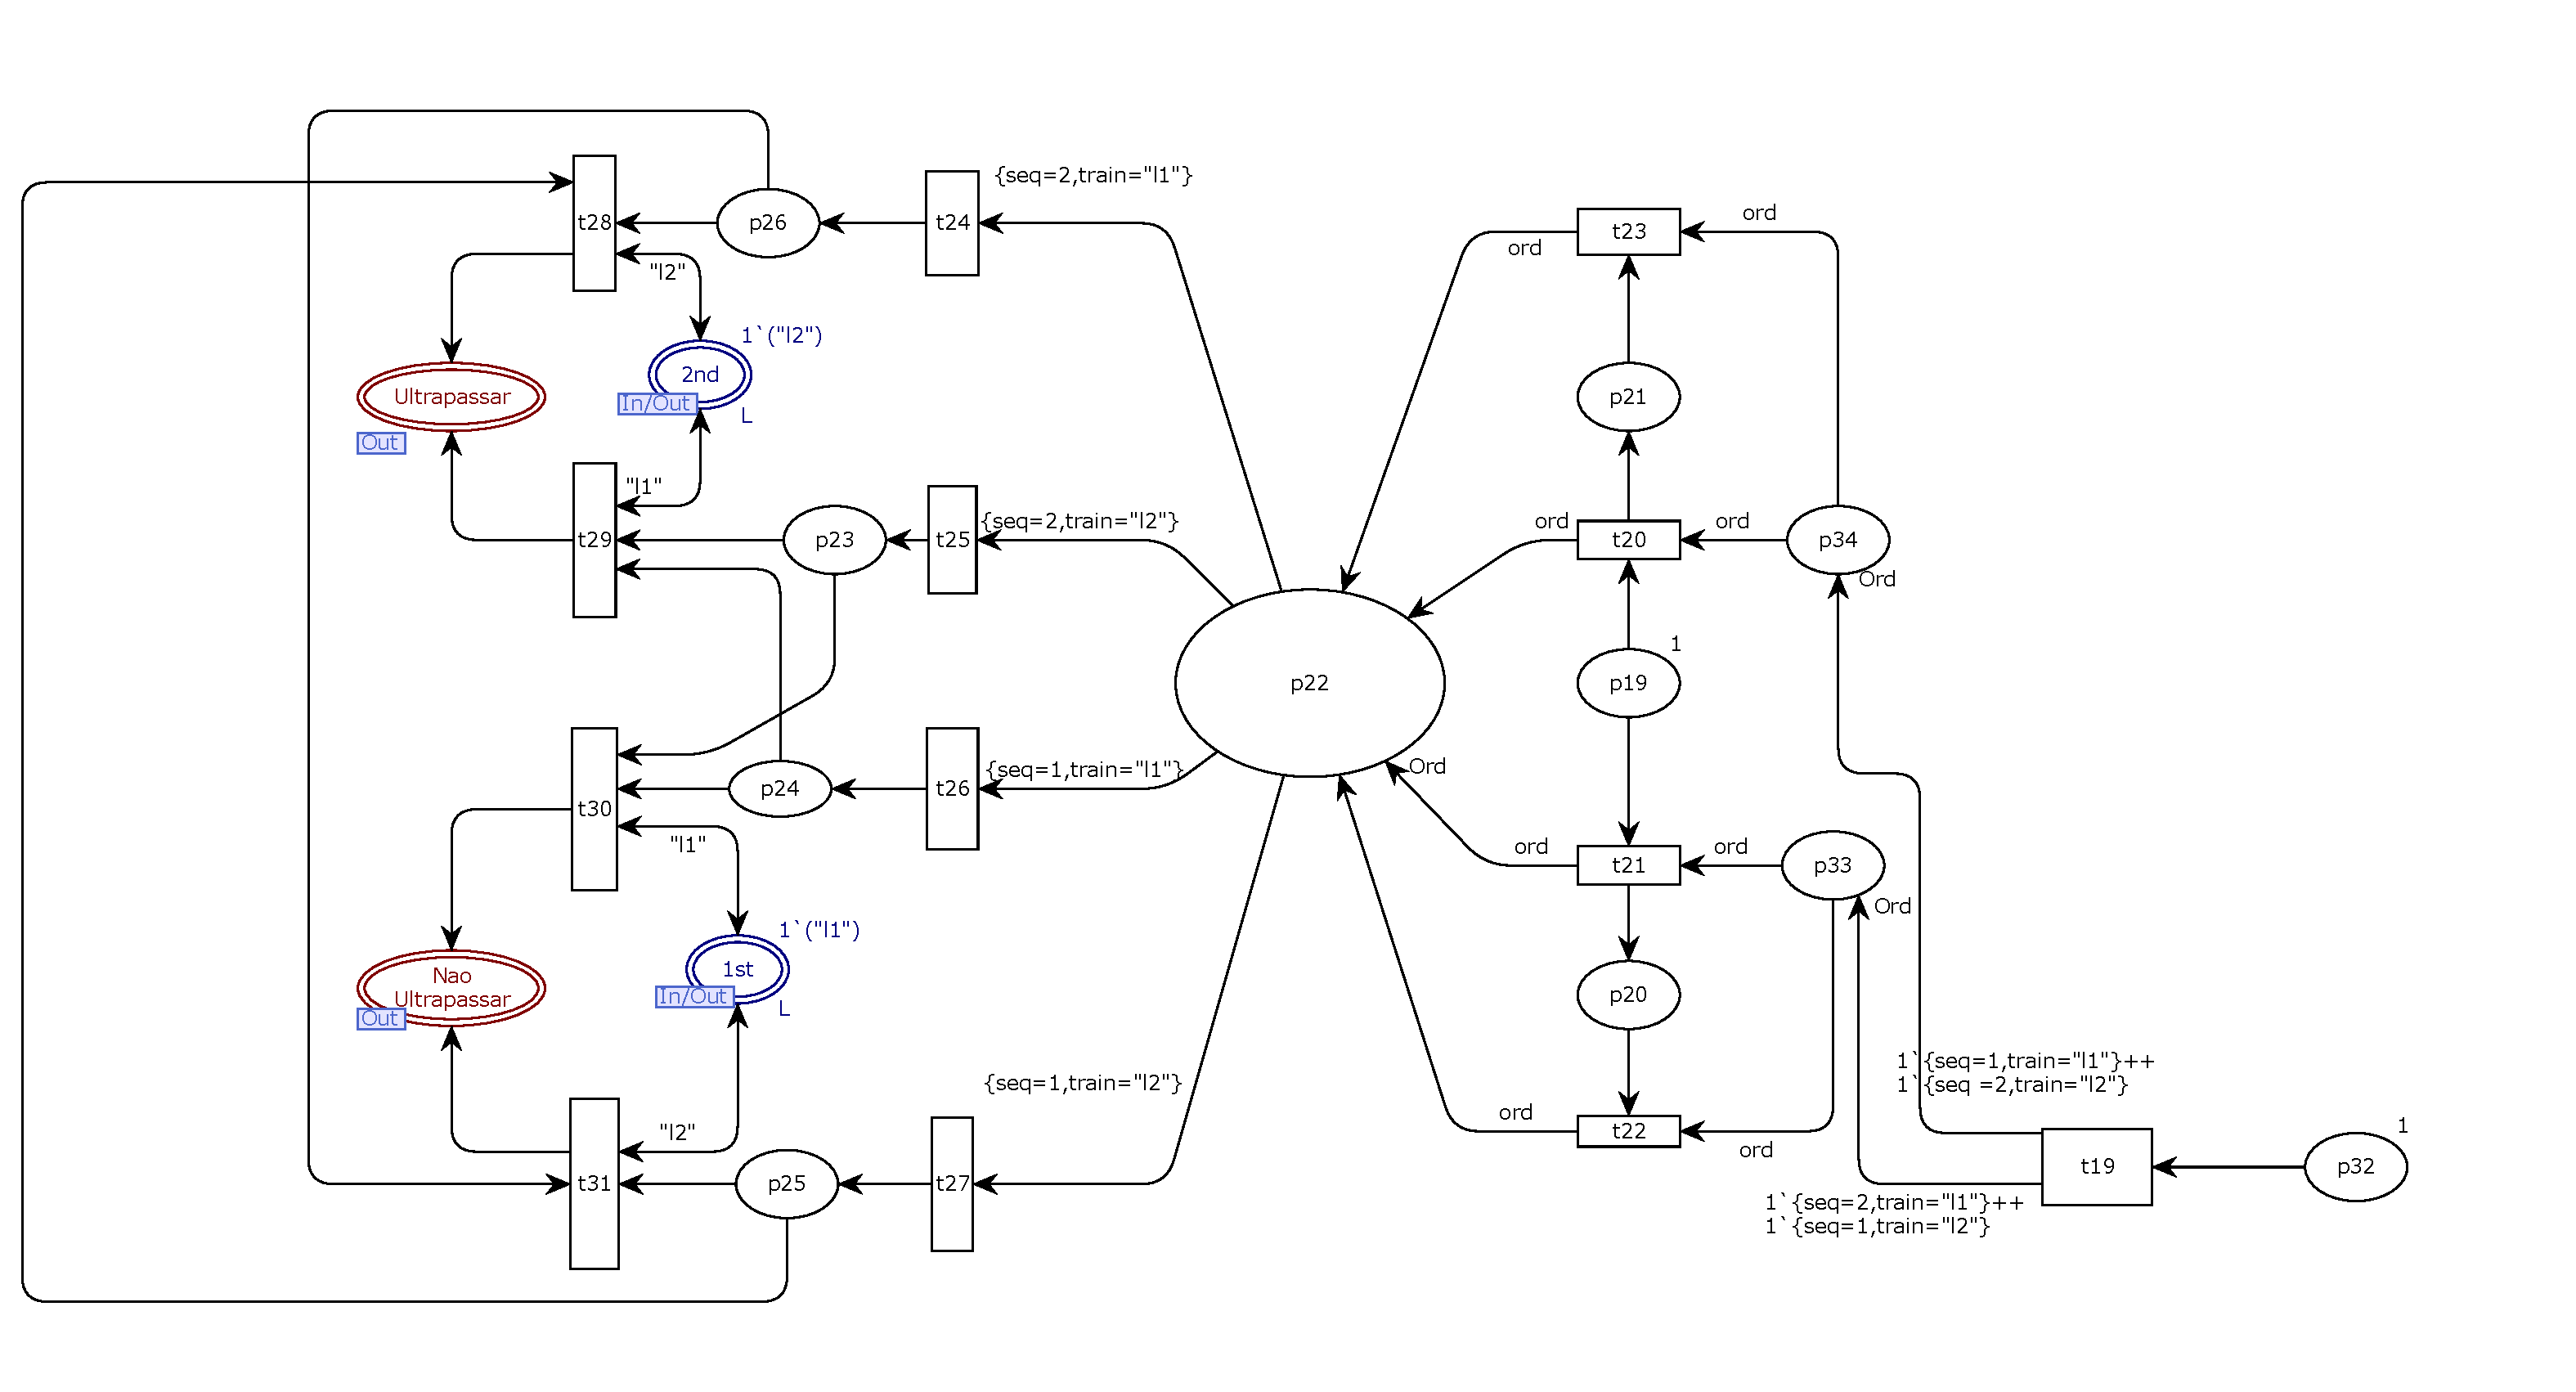
\includegraphics[width=1\linewidth]{figures/Simulation/Modelagem/geracao_ordem.eps}
    \legend{Fonte: Elaborado pelo autor.}
\end{figure}

Após gerado o comando de \textit{Ultrapassar} ou \textit{Não Ultrapassar} é necessário modelar o reestabelecimento da rede para que possa ser gerado novamente os comandos e não haja travamento da rede. O reestabelecimento é demonstrado na figura \ref{fig:restabelecer_ordem}, tal que após gerado os comandos que podem vir de qualquer uma das quatro transições $t_{28}, t_{29}, t_{30}, t_{31}$ a transição $t_32$ transfere uma ficha para $p_{28}$ que ativará a transição $t_{33}$ no momento de reestabelecer a ordem e uma ficha para o $p_{29}$ responsável por retirar a ficha que não foi utilizada durante a escolha aleatória de ordem.

\begin{figure}[ht]
    \centering
    \caption{Máscara referente ao restabelecimento do componente de Ordem na RPC}
    \label{fig:restabelecer_ordem}
    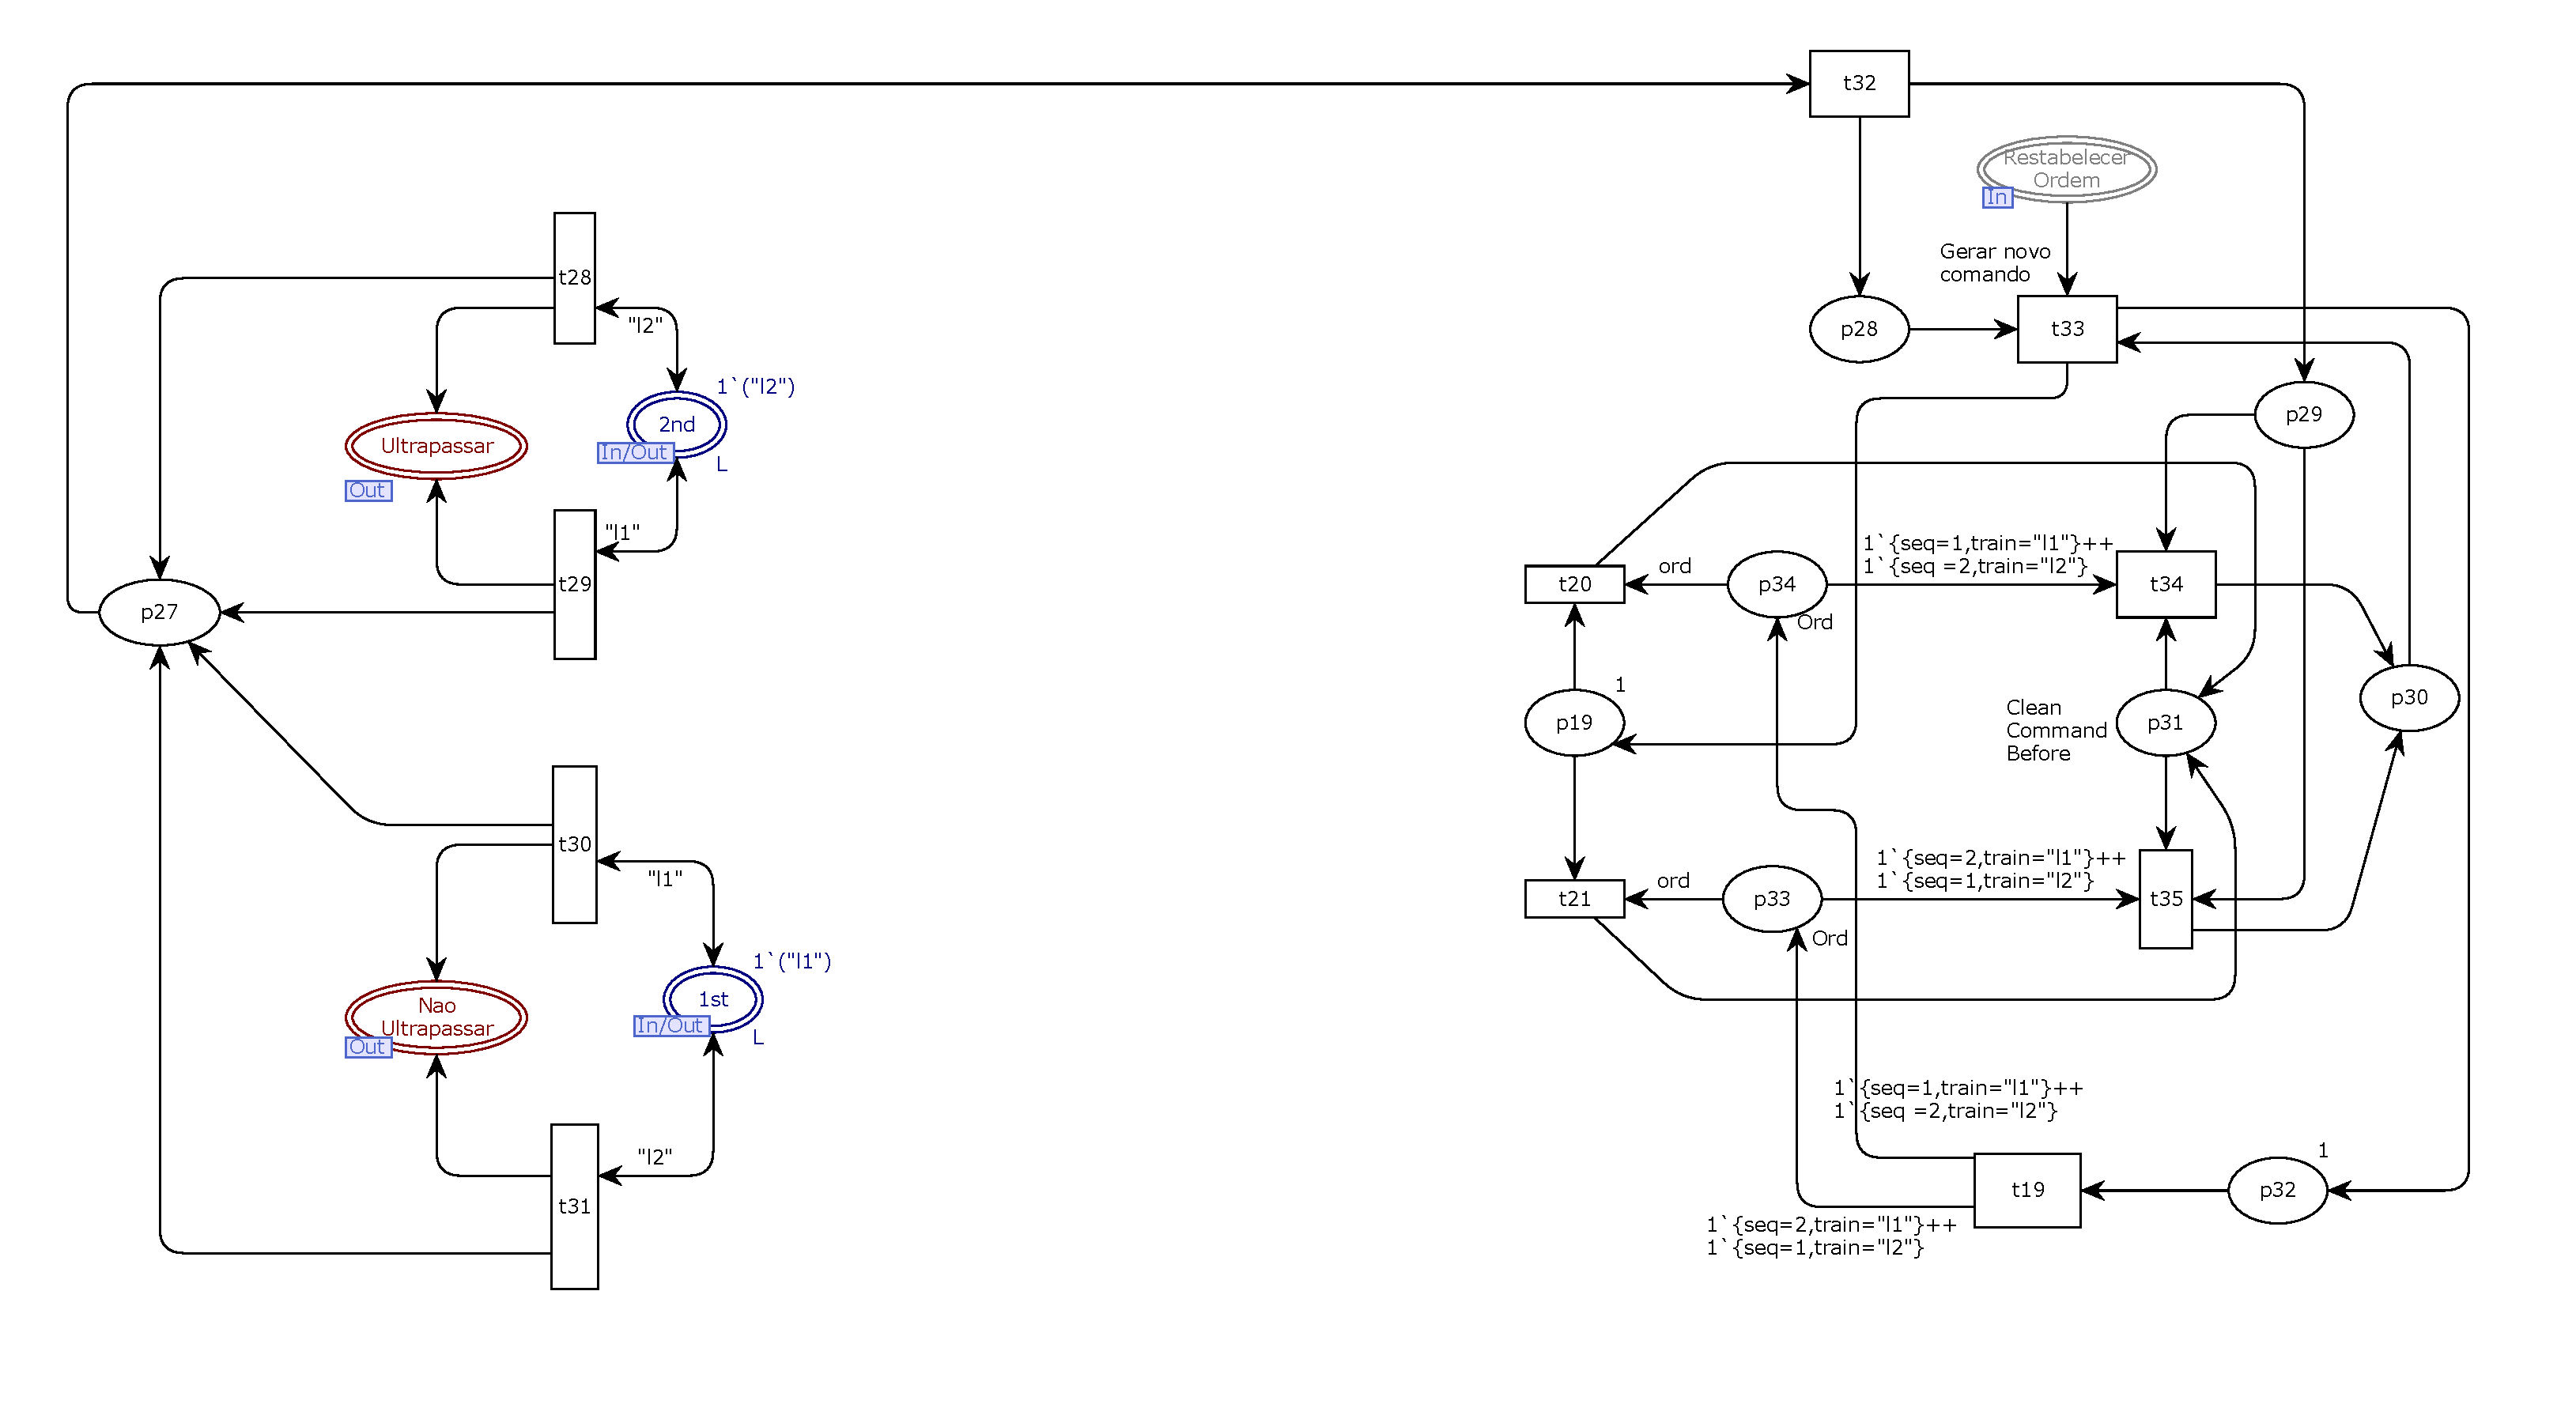
\includegraphics[width=1\linewidth]{figures/Simulation/Modelagem/restabelecer_ordem.eps}
    \legend{Fonte: Elaborado pelo autor.}
\end{figure}

O ultimo componente hierárquico da rede é o de \textit{Inverter Ordem}, responsável por atualizar os lugares de $1_{st}$ e $2_{nd}$, dado pela RPC representada na figura \ref{fig:inverter_ordem}. Note que ao chegar o comando de atualizar ordem caso haja uma ficha em ultrapassar, é ativado a transição $t_{36}$ que tem como objetivo retirar a ficha que estava em $2_{nd}$ guardar temporariamente em $p_{37}$ enquanto a ficha que estava em primeiro lugar é transferida para o segundo lugar e por fim é atualizado o primeiro lugar.
Caso não tenha ocorrido ultrapassagem a transição $t_{37}$ é acionada enviando o comando de \textit{Restabelecer a Rede} para a hierarquia a cima.

\begin{figure}[ht]
    \centering
    \caption{Máscara referente ao restabelecimento do componente de Ordem na RPC}
    \label{fig:inverter_ordem}
    \includegraphics[width=1\linewidth]{figures/Simulation/Modelagem/inverter_ordem.eps}
    \legend{Fonte: Elaborado pelo autor.}
\end{figure}

\section{Controle Cooperativo aplicado a Multiagentes}
Posteriormente à detalhada modelagem do sistema na seção \ref{sec:model_RPC} que foi definida os principais eventos do sistema, além da arquitetura da rede que gera algumas regras para o deslocamento dos vagões é buscada um controle de nível superior responsável por otimizar a referência de posição de cada vagão. Para o desenvolvimento do controle cooperativo entre os vagões com o objetivo de evitar colisões e promover a otimização das trajetórias é importante garantir que as transições na rede de petri possuem acionamentos praticamente instantâneos não influenciando assim de forma significativa na dinâmica do sistema.



\chapter{Conclusão}
\label{chap:conclusion}
O método de modelagem e controle proposto foi realizado no problema de uma planta industrial envolvendo a sincronia e formação de um grupo de autômatos ao longo de trajetórias pré definidas, em que a partir de alguns eventos modelados pela rede de Petri foi alterado a formação do grupo de autômatos assim como os pontos de sincronia.
O método se apresentou como uma técnica viável e eficiente, pois para aplicações de sistemas com muitos agentes o controle por consenso se apresenta como uma implementação simples sem grande uso de recurso matemático que fornece a sincronia necessária para aplicação de formação ordenada do grupo de autômatos.
No ponto de vista de robustez e adaptabilidade do sistema, observou-se que cada agente respeita as limitações dos agentes vizinhos, seja ela de posição de velocidade, evitando assim colisões e independente da mudança da dinâmica de um agente todo o sistema tem sua dinâmica adaptada, trazendo assim uma sincronia entre os diferentes agentes com diferentes dinâmicas ao longo do sistema.
A principal contribuição desse trabalho é a técnica conjunta de modelagem e controle que  diminui o processamento local em cada agente deixando assim as lógicas de processamento centralizada em um sistema supervisório modelado via rede de petri, além de uma lógica de controle de baixo custo computacional, todavia é necessário uma ótima comunicação entre os agentes,pois a base do controle é dada pela sincronia entre os estados do agente vizinho.
	

%Elementos pós-textuais	
\bibliography{3-pos-textuais/referencias}
% \imprimirglossario
% \imprimirapendices
% Adicione aqui os apendices do seu trabalho
% % \apendice{EXEMPLO DE APÊNDICE}
% \label{ap:A}


% % \apendice{ Questionário utilizado para}
% \label{ap:B}

% \begin{questao}
% 	\item Esta é a primeira questão com alguns itens:
% 		\begin{enumerate}
% 			\item Este é o primeiro item
% 			\item Segundo item
% 		\end{enumerate}
% 	\item Esta é a segunda questão:
% 		\begin{enumerate}
% 			\item Este é o primeiro item
% 			\item Segundo item
% 		\end{enumerate}
% 	\item Lorem ipsum dolor sit amet, consectetur adipiscing elit. Nunc dictum sed tortor nec viverra. consectetur adipiscing elit. Nunc dictum sed tortor nec viverra.
% 		\begin{enumerate}
% 			\item consectetur
% 			\item adipiscing
% 			\item Nunc
% 			\item dictum
% 		\end{enumerate}
% \end{questao}

% % \apendice{ Códigos-fontes utilizados para}
% \label{ap:C}

% \lstinputlisting[language=C++,caption={Hello World em C++}]{figuras/main.cpp}


% \begin{lstlisting}[language=Java,caption={Hello World em Java}]
% public class HelloWorld {
% 	public static void main(String[] args) {
% 		System.out.println("Hello World!");
% 	}
% }
% \end{lstlisting}



%\imprimiranexos
% Adicione aqui os anexos do seu trabalho
%% \anexo{ Exemplo de um anexo}
% \label{an:ex_anexo_a}

% \textcolor{red}{Colocar como anexo o passo a passo de integração do matlab com o coppelia.}




%% \anexo{ Exemplo de um anexo em PDF}
% \label{an:ex_anexo_b}

% O autor pode anexar um \gls{PDF}, traduzido como formato portátil de documento. Veja o código fonte utilizado para anexar o arquivo ``Sikasil.pdf'' que foi colocado dentro da pasta ``anexos'' que por sua vez está dentro da pasta ``elementos-pos-textuais''. Tenha muita atenção na hora de especificar o local do arquivo. Recomenda-se não utilizar caracteres especiais para nomear pastas e, principalmente, arquivos. 

% Pode-se fazer uma descrição sucinta do arquivo anexado.

%Comando para incluir um arquivo em PDF:
% \includepdf[pages={-}]{3-pos-textuais/anexos/Sikasil.pdf}

		

\imprimirindice

\end{document}